\documentclass{momento}
\usepackage{physicsplus}
%\usepackage{danielgroups}
%\usepackage{tikz-3dplot}

\usepackage{gnuplot-lua-tikz}
\newcommand{\python}[2]{ python scripts/legendre.py -n #1 -m #2}

\renewcommand{\dyad}[1]{\boldsymbol{\rm #1}}
\usepgfplotslibrary{polar}
\title{Mathematical Methods for Physics}
\author{Daniel Williams}
%\pubyear{2014}
\setcounter{section}{-1}

\begin{document} \maketitle

\begin{tikzpicture}[overlay]
   \coordinate (A) at (-3,5.5);
   \begin{axis} [opacity=0.7,hide axis,width=10in, height=3in,xmin=0, xmax=20, at=(A)]
    \addplot gnuplot[fill, raw gnuplot, id=bess, mark=none, muted-blue, ultra thick]{
      set xrange[0:20];
      plot besj0(x);
    } \closedcycle;
     \addplot gnuplot[opacity=0.7,fill,raw gnuplot, id=bess2, mark=none, muted-green, ultra thick]{
      set xrange[0:20];
      plot besj1(x);
    } \closedcycle;
    \addplot gnuplot[opacity=0.7,fill,raw gnuplot, id=bess3, mark=none, muted-orange, ultra thick]{
      set xrange[0:20];
      fac(n) = (int(n)==0) ? 1.0 : int(n) * fac(int(n)-1.0);
      besj_eps = 0.1;
      besj(n,x) = (n==0) ? besj0(x) : (n==1) ? besj1(x) : (abs(x)<besj_eps*(n+1)) ? (x/2.0)**n/fac(n) : 2*(n-1)/x*besj(n-1,x) - besj(n-2,x);
      plot besj(2,x);
    } \closedcycle;
    \addplot gnuplot[opacity=0.7,fill,raw gnuplot, id=bess4, mark=none, accent-purple, ultra thick]{
      set xrange[0:20];
      fac(n) = (int(n)==0) ? 1.0 : int(n) * fac(int(n)-1.0);
      besj_eps = 0.1;
      besj(n,x) = (n==0) ? besj0(x) : (n==1) ? besj1(x) : (abs(x)<besj_eps*(n+1)) ? (x/2.0)**n/fac(n) : 2*(n-1)/x*besj(n-1,x) - besj(n-2,x);
      plot besj(3,x);
    }\closedcycle;
    \addplot gnuplot[opacity=0.7,fill,raw gnuplot, id=bess5, mark=none, accent-red, ultra thick]{
      set xrange[0:20];
      fac(n) = (int(n)==0) ? 1.0 : int(n) * fac(int(n)-1.0);
      besj_eps = 0.1;
      besj(n,x) = (n==0) ? besj0(x) : (n==1) ? besj1(x) : (abs(x)<besj_eps*(n+1)) ? (x/2.0)**n/fac(n) : 2*(n-1)/x*besj(n-1,x) - besj(n-2,x);
      plot besj(4,x);
    }\closedcycle;
  \end{axis}
\end{tikzpicture}

% \begin{abstract}
%   These notes are based on a lecture course taught by Professor C
%   Davies and Dr Douglas MacGregor during the winter term of the 2013 session.
% \end{abstract}
\tableofcontents

\chapter{Partial Differential Equations}
\label{cha:part-diff-equat}

\section{Einstein Summation Convention}
\label{sec:einsteinsummation}

Consider a three-dimensional vector space, $\mathsf{V}$, over the
field of real numbers, $\mathbb{R}$.  Any point in the space can be
described by an ordered set of three numbers, $(x_1, x_2, x_3)$, known
as coordinates, such that
\[ \vec{A} = (x_1, x_2, x_3) \cdot
\begin{pmatrix} \vec{e_1} \\ \vec {e_2} \\ \vec{e_3}
\end{pmatrix}
\]
where $\vec{A}$ is any vector in $\mathsf{V}$, and $\vec{e_1}$, $\vec
{e_2}$, and $\vec{e_3}$ constitute a basis for $\mathsf{V}$.

This can be expressed in a more compact form by adopting the {\em
  Einstein summation convention}. In this system the summation sign,
$\sum$, is omitted, and replaced with repeated indices, viz.
\[ \vec{A} = A_i \vec{e_i} = \sum_{i=1}^3 A_i\vec{e_i} \] here $i$ is
a repeated index, and so the summation over it is implicit.  This
allows the definition of a number of vector calculus operations in a
more compact way.

\subsection{Operations}
\label{sec:operations}


\subsubsection{Dot Product}
\label{sec:dotproduct}

\begin{equation}
  \label{eq:dotprod}
  \vec{a} \cdot \vec{b} = a_\theta b_\theta
\end{equation}

\subsubsection{Total Differential}
\label{sec:totaldiff}

\begin{equation}
  \label{eq:totaldifferential}
  \dif{f} = \frac{\partial f}{\partial x_\theta} \dif{x_\theta}
\end{equation}

\subsubsection{Matrix Multiplication}
\label{sec:matrixmult}

\begin{equation}
  \label{eq:matmult}
  a_{ij} = b_{i \theta} c_{\theta j}
\end{equation}

\subsubsection{Cross Product}
\label{sec:crossprod}

\begin{equation}
  \label{eq:crossprod1}
  [ \vec a \times \vec b]_i = \epsilon_{i \theta \phi} a_{\theta} b_{\phi}
\end{equation}
\begin{equation}
  \label{eq:crossprod2}
  \vec{a} \times \vec{b} = \epsilon_{i \theta \phi} a_{\theta} b_{\phi} \vec{e_{i}}
\end{equation}
Here $\epsilon_{i \theta \phi}$ is the Levi-Civita tensor, and takes
values

\begin{equation}
  \label{eq:levitcivita}
  \epsilon_{i \theta \phi} = \left\{ 
    \begin{array}{rl}
      0 & \text{if any indices are repeated.} \\
      1 & \text{if indices are a cyclic permutation of } (1,2,3). \\
      -1 & \text{if indices are a cyclic permutation of } (1,3,2). 
    \end{array}\right.
\end{equation}
There is a simple relationship between this tensor and the Kronecker
delta,
\begin{equation}
  \label{eq:deltalevi}
  \epsilon_{\theta j k } \epsilon_{\theta l m} = \delta_{jl} \delta_{k m} - \delta_{j m} \delta_{l k}
\end{equation}

\subsection{Del Operators}
\label{sec:deloperators}
The gradient is now expressed:
\begin{equation}
  \label{eq:grad}
  \nabla = \vec e_i \frac{\partial }{\partial x_i}
\end{equation}
The divergence:
\begin{equation}
  \label{eq:divergence}
  \nabla \cdot \vec{A}(\vec{r}) = \frac{\partial A_i(\vec{r})}{\partial x_i}
\end{equation}
and the curl:
\begin{equation}
  \label{eq:curl}
  \nabla \times \vec{A}(\vec{r}) = \epsilon_{ijk} \frac{\partial A_j(\vec{r})}{\partial x_i} \vec{e_k}
\end{equation}
\begin{example}
  Consider
  \[ \left[ \vec{a} \times ( \vec{b} \times \vec{c} ) \right]_m \]
  using the summation convention,
  \begin{align*} \left[ \vec{a} \times ( \vec{b} \times \vec{c} )
    \right]_m
    &= \epsilon_{m \alpha \beta} a_{\alpha} \epsilon_{\beta \gamma \delta} b_{\gamma} c_{\delta} \\
    &= \epsilon_{\beta m \alpha} \epsilon_{\beta \gamma \delta} a_{\alpha} b_{\gamma} c_{\delta} \\
    &= (\delta_{m \delta}\delta_{\alpha \delta} - \delta_{m \delta} \delta_{a \gamma}) a_{\alpha} b_{\gamma} c_{\delta}\\
    &=  (a_{\alpha}c_{\alpha}) b_m - (a_{\alpha}b_{\alpha}) c_m \\
    &= \left[ (\vec a \cdot \vec c) \vec b - (\vec a \cdot \vec b)
      \vec c \right]_{m}
  \end{align*}
\end{example}
Note, \[ \delta_{i\theta} a_{\theta} = a_i \]
\begin{example}
  \begin{align*}
    \nabla \times ( \nabla \phi ) &= \epsilon_{m\alpha \beta} \frac{\partial }{\partial x_a} \frac{\partial \phi}{\partial x_{\beta}}\\
    &= 0
  \end{align*}
  This arises because the Levi-Civita tensor is anti-symmetric, but
  the two partial derivatives are symmetric.
\end{example}
\begin{example}
  \begin{align*}
    \vec A \cdot \vec B \times \vec C &= A_{\alpha}\epsilon_{\alpha \beta \gamma} B_{\beta} C_{\gamma} \\
    &= C_{\gamma} \epsilon_{\gamma \alpha \beta} A_{\alpha} B_{\beta} \\
    &= C_{\gamma} [\vec A \times \vec B]_{\gamma} \\
    &= C \cdot [ \vec A \times \vec B]
  \end{align*}
\end{example}

\section{Curvilinear coordinates}
\label{sec:curvi}

A curvilinear coordinate system is a coordinate system over a space in
which the coordinate lines may be curved, and are related to a
Cartesian coordinate system by a bijection.  In physics, laws are
independent of reference frame and of coordinate system, which allows
the use of the most appropriate coordinate system for a specific
situation---for example, if a problem has spherical symmetry it is
likely to be easiest to solve in spherical polar coordinates.

\subsection{Spherical Polar Coordinates}
\label{sec:sphpol}

\begin{minipage}[!]{\linewidth}
  \noindent\begin{minipage}[!]{0.45\linewidth}
    \definecolor{accent-pink}{HTML}{C3325F}
\definecolor{accent-red}{HTML}{9d261d}
\definecolor{accent-purple}{HTML}{7a43b6}
\definecolor{muted-blue}{HTML}{195073}
\definecolor{muted-green}{HTML}{7F8C1F}
\definecolor{muted-orange}{HTML}{EE913F}
\begin{tikzpicture}
  \draw [->, thick, accent-red] (0,0) -- (0,2.5);
  \draw [->, thick, accent-red] (0,0) -- (-1, -1.5);
  \draw [->, thick, accent-red] (0,0) -- (3,0);
 
  \draw [->>, ultra thick, accent-purple] (0,0) -- (2,2);
  \draw [dashed, muted-orange] (2,2) -- (2, -1);
  \draw [<->] (0,0) -- (2,-1) node [below,] {$r$};
 
  \draw [<->] (0,0.7) arc (45:0:0.7) node [yshift=8pt,above]{$\theta$};
  \draw [<->] (.5, -.3) arc (300:255:1) node [yshift=-2pt, below] {$\phi$};
\end{tikzpicture}
  \end{minipage}
  \hfill
  \noindent\begin{minipage}[!]{0.45\linewidth}
    They are related to Cartesian coordinates by the transformations:
    \begin{align}
      x &= r \sin \theta \cos \phi \label{eq:sph1}\\
      y &= r \sin \theta \sin \phi \label{eq:sph2}\\
      z &= r \cos \theta \label{eq:sph3}
    \end{align}
    \hfill \vfill
  \end{minipage}
\end{minipage}

\subsection{Cylindrical Polar Coordinates}
\label{sec:cylpol}
\begin{minipage}[!]{\linewidth}
  \noindent\begin{minipage}[!]{0.45\linewidth}
    \definecolor{accent-pink}{HTML}{C3325F}
\definecolor{accent-red}{HTML}{9d261d}
\definecolor{accent-purple}{HTML}{7a43b6}
\definecolor{muted-blue}{HTML}{195073}
\definecolor{muted-green}{HTML}{7F8C1F}
\definecolor{muted-orange}{HTML}{EE913F}
\begin{tikzpicture}
  \draw [->, thick, accent-red] (0,0) -- (0,2.5);
  \draw [->, thick, accent-red] (0,0) -- (-1, -1.5);
  \draw [->, thick, accent-red] (0,0) -- (3,0);
 
  \draw [->>, ultra thick, accent-purple] (0,2) -- (2,1.5);
  \draw [dashed, muted-orange] (2,1.5) -- (2, -1);
  \draw [<->] (0,0) -- (2,-1) node [below,] {$r$};
  \draw [<->] (-.1,0) -- (-.1,2) node [left] {$z$};
  \draw [<->] (.5, -.3) arc (300:255:1) node [yshift=-2pt, below] {$\phi$};
\end{tikzpicture}
  \end{minipage}
  \hfill
  \noindent\begin{minipage}[!]{0.45\linewidth}
    They are related to Cartesian coordinates by the transformations:
    \begin{align}
      x &= r \cos \theta \label{eq:cyl1}\\
      y &= r \sin \theta \label{eq:cyl2}\\
      z &= z \label{eq:cyl3}
    \end{align}
    \hfill \vfill
  \end{minipage}
\end{minipage}

\subsection{Unit vectors and scale factors}
\label{sec:unitsscale}

In any coordinate system there is a concept of distance, which is
independent of the choice of coordinate system.  In Cartesian
coordinates this is
\[ \dif{s}^2 = \dif{x}^2 + \dif{y}^2 + \dif{z}^2 = \dif{r}\cdot
\dif{r} \] where $\dif{r}$ is the inifinitessimal line element.

Consider a general coordinate system described by $q_i$, related to
Cartesian coordinates via
\[ x_i = f_i (q_1, q_2, q_3) \] As $q_i$ is changed the position
vector $\vec r$ will move:
\[ \frac{\partial \vec r}{\partial q_i} = h_{q_i} \vec{e}_{q_i} \] The
magnitude of $\frac{\partial \vec r}{\partial q_i}$ is the scale
factor, $h_{q_i}$, and the basis vector is the unit vector in the
direction of $\frac{\partial \vec r}{\partial q_i}$.  We can then
define the infinitessimal line element,
\begin{equation}
  \label{eq:infinitessimalcurve}
  \dif{s}^2 = \sum_{i, j} g_{ij} \dif{q_i} \dif{q_j}
\end{equation}
Where $g_{ij}$ is the metric for the geometry we are considering.  The
volume element is then
\begin{equation}
  \label{eq:volumecurvi}
  \dif{V} = \dif{s}_{1} + \dif{s}_2 + \dif{s}_3 = h_{q_1}h_{q_2}h_{q_3} \dif{q_1} \dif{q_2} \dif{q_3}
\end{equation}
\begin{example}[Spherical Polar Coordinates]
  From the relations in equations (\ref{eq:sph1}) to (\ref{eq:sph3}),
  and considering that
  \[ \vec{r} = x \vec{e_x} + y \vec{e_y} + z \vec{e_{z}} \] Then,
  \begin{align*}
    \frac{\partial \vec r}{\partial r}
    &= \frac{\partial x}{\partial r} \vec{e_x} + \frac{\partial y}{\partial r} \vec{e_y} + \frac{\partial z}{\partial r} \vec{e_z} \\
    &= \sin \theta \cos \phi \vec{e_{x}} + \sin\theta \sin \phi \vec{e_y} + \cos \theta \vec{e_z} = h_r\vec{e_r} \\
    \frac{\partial \vec r}{\partial \theta}
    &= \frac{\partial x}{\partial \theta} \vec{e_x} + \frac{\partial y}{\partial \theta} \vec{e_y} + \frac{\partial z}{\partial \theta} \vec{e_z} \\
    &= r \cos \theta \cos \phi \vec{e_x} + r \cos \theta \sin \phi \vec{e_y} - r \sin \theta \vec{e_z} = h_{\theta}\vec{e_{\theta}} \\
    \frac{\partial \vec r}{\partial \phi}
    &= \frac{\partial x}{\partial \phi} \vec{e_x} + \frac{\partial y}{\partial \phi} \vec{e_y} + \frac{\partial z}{\partial \phi} \vec{e_z} \\
    &= - \sin \theta \sin \phi \vec{e_{x}} + r \sin\theta \cos \phi \vec{e_y} = h_{\phi}\vec{e_{\phi}} \\
  \end{align*}
  Then the scale factors are
  \begin{align*}
    h_r &= \left| \frac{\partial \vec r}{\partial r} \right| = 1\\
    h_{\theta} &= \left| \frac{\partial \vec r}{\partial \theta} \right| = r\\
    h_{\phi} &= \left|  \frac{\partial \vec r}{\partial \phi} \right| = r \sin \theta\\
  \end{align*}
  Also, the volume element,
  \[ \dif{V} = r^2 \sin \theta \dif{r} \dif{\theta} \dif{\phi} \] and
  the square of the infinitessimal line element,
  \[ \dif{s}^2 = \dif{r}^2 + r^2 \dif{\theta}^2 + r^2 \sin^2 \theta
  \dif{\phi^2} \]
\end{example}

\subsection{Del Operators}
\label{sec:delcurvi}

\subsubsection{Gradient}
\label{sec:gradcurvi}

The gradient in the direction of $\vec{e_{q_1}}$ is
\begin{equation} \label{eq:dirgradcurvi} \nabla_{q_i} =
  \frac{\partial}{\partial s_i} = \frac{1}{h_{q_i}}
  \frac{\partial}{\partial q_i}
\end{equation}
thus, the total gradient operator is
\begin{equation}
  \label{eq:gradincurvi}
  \nabla = \sum_i \vec{e_{q_i}} \frac{\partial}{\partial s_i} = \sum_i \vec{e_{q_i}} \frac{1}{h_{q_i}} \frac{\partial}{\partial q_i}
\end{equation}

\subsubsection{Divergence}
\label{sec:divcurvi}

We can define the divergence from the gradient, since
\[ \nabla \cdot \vec{A} = \nabla \cdot \left( \sum_j A_j \vec{e_{q_j}}
\right) \] clearly we need $\nabla \cdot \vec{e_{q_j}}$ to continue;
from equation (\ref{eq:dirgradcurvi}),
\[ \nabla \cdot q_j = \sum_i \frac{1}{h_{q_i}} \frac{\partial
  q_j}{\partial q_i} = \sum_i \vec{e_{q_i}} \frac{1}{h_{q_i}}
\delta_{ij} = \vec{e_{q_j}} \frac{1}{h_{q_j}} \] Thus,
\[\vec{e_{q_j}} = h_{q_j} \nabla q_j \]
The basis vectors form a right-handed set, so,
\[e_{q_1} \times e_{q_2} = e_{q_3} \] and
\[\nabla q_1 \times \nabla q_2 =
\frac{\vec{e_{q_3}}}{h_{q_1}h_{q_2}}\] Considering that $\curl(\grad)
= 0$,
\begin{align*} \nabla \cdot (\nabla_{q_1} \times \nabla_{q_2}) &=
  \nabla q_2 \cdot (\nabla \times \nabla q_1) - \nabla q_1 \cdot (
  \nabla \times \nabla q_2) \\ &= 0
\end{align*}
So
\[ \nabla \cdot \left( \frac{\vec{e_{q_3}}}{h_{q_1} h_{q_2}} \right) =
0 \] and the same argument applies for cyclic permutations,
\[ \nabla \cdot \left( \frac{\vec{e_{q_3}}}{h_{q_1} h_{q_2}} \right) =
\nabla \cdot \left( \frac{\vec{e_{q_1}}}{h_{q_2} h_{q_3}} \right) =
\nabla \cdot \left( \frac{\vec{e_{q_2}}}{h_{q_3} h_{q_1}} \right) =
0 \] Then returning to
\begin{align*}
  \nabla \cdot \vec{A} &= \nabla \cdot \left( \sum_j A_j \vec{e_{q_j}} \right) &\\
  &= \nabla \cdot \left\{ [h_{q_1}h_{q_2}A_1] \left[
      \frac{\vec{e_{q_1}}}{h_{q_2} h_{q_3}} \right] \right.
  &+& [h_{q_3}h_{q_1}A_2] \left[ \frac{\vec{e_{q_2}}}{h_{q_3} h_{q_1}} \right] \\
  &&+&\left.[h_{q_1} h_{q_2}A_3]  \left[ \frac{\vec{e_{q_3}}}{h_{q_1} h_{q_2}} \right]  \right\} \\
  &= \left[ \frac{\vec{e_{q_1}}}{h_{q_2} h_{q_3}} \right] \cdot \nabla
  [h_{q_1}h_{q_2}A_1]
  &+&\left[ \frac{\vec{e_{q_2}}}{h_{q_3} h_{q_1}} \right] \cdot \nabla [h_{q_3}h_{q_1}A_2]\\
  &&+&\left[ \frac{\vec{e_{q_3}}}{h_{q_1} h_{q_2}} \right]\cdot \nabla
  [h_{q_1}h_{q_2}A_3]
\end{align*}
Since
\[\vec{e_{q_i}} \cdot \nabla = \frac{1}{h_{q_i}}
\frac{\partial}{\partial q_i}\],
\begin{equation}
  \label{eq:divincurvi}
  \begin{split}
    \nabla \cdot \vec{A} = \frac{1}{h_{q_1}h_{q_2}h_{q_3}} \left( \frac{\partial}{\partial q_1} (h_{q_2} h_{q_3} A_1) \right. \\
    + \left. \frac{\partial}{\partial q_2} (h_{q_3} h_{q_1} A_2) +
      \frac{\partial}{\partial q_3} (h_{q_2} h_{q_1} A_3) \right)
  \end{split}
\end{equation}
\subsubsection{Curl}
\label{sec:curlcurvi}
The curl can be derived from earlier results,
\begin{align*}
  \nabla \times \vec{A} &=&& \nabla \times \left( \sum_j A_j \vec{e_{q_j}} \right) \\
  &=&& \nabla \times \left(
    \begin{matrix}
      [h_{q_1}A_1] \qty[\frac{\vec{e_{q_1}}}{h_{q_1}} ] &+
      [h_{q_2}A_2] \qty[ \frac{\vec{e_{q_2}}}{h_{q_2}} ] \\ &+
      [h_{q_3}A_3] \qty[ \frac{\vec{e_{q_3}}}{h_{q_3}} ]
    \end{matrix}
  \right) \\
  &= && - \left[ \frac{\vec{e_{q_1}}}{h_{q_1}} \right] \times \nabla
  (h_{q_1}A_1)
  - \left[ \frac{\vec{e_{q_2}}}{h_{q_2}} \right] \times \nabla (h_{q_2}A_2) \\
  &&& - \left[ \frac{\vec{e_{q_3}}}{h_{q_3}} \right] \times \nabla
  (h_{q_3}A_3)
\end{align*}
so,
\begin{equation}
  \label{eq:curlincurvi}
  \nabla \times \vec{A} = 
  \frac{1}{h_{q_1}h_{q_2}h_{q_3}}
  \begin{vmatrix}
    h_{q_1} \vec{e_1}              & h_{q_2} \vec{e_2}              & h_{q_3} \vec{e_{3}}             \\
    \frac{\partial}{\partial q_1} & \frac{\partial}{\partial q_2} & \frac{\partial}{\partial q_3} \\
    h_{q_1} A_1 & h_{q_2} A_2 & h_{q_3} A_3
  \end{vmatrix}
\end{equation}

\subsubsection{Laplacian}
\label{sec:laplaciancurvi}

\begin{equation}
  \label{eq:laplacianincurvi}
  \begin{split}
    \nabla^2 = \frac{1}{h_{q_1}h_{q_2}h_{q_3}} 
    \bigg( \pdv{q_1} \qty[ \frac{h_{q_2}h_{q_3}}{h_{q_1}} \pdv{q_1} ] 
    +  \pdv{q_2} \qty[ \frac{h_{q_3}h_{q_1}}{h_{q_2}} \pdv{q_2} ] \\
    +  \pdv{q_3} \qty[ \frac{h_{q_2}h_{q_1}}{h_{q_1}} \pdv{q_3} ] \bigg) 
  \end{split}
\end{equation}
\section{Partial Differential Equations in Curvlinear Coordinate
  Systems}
\label{sec:curvipde}

\subsection{Common Partial Differential Equations}
\label{sec:commonpdes}

There are a number of common PDEs which it is useful to know.

\subsubsection{Laplace's Equation} \label{sec:laplacepde}

\begin{equation}
  \label{eq:laplace}
  \nabla^2 \phi(\vec{r}) = 0
\end{equation}
This equation is used in electromagnetism, gravitation, hydrodynamics,
and heat flow in situations where no sources or sinks exist.

\subsubsection{Poisson's Equation} \label{sec:poissonpde}

\begin{equation}
  \label{eq:poisson}
  \nabla^2 \phi(\vec{r}) = f(\vec{r})
\end{equation}
This is used in the same situations as Laplace's equation,
(\ref{eq:laplace}), only when there {\em are} sources or sinks,
described by the scalar field $f$.
\begin{example}
  One of Maxwell's equations is
  \[ \nabla \cdot \vec{E} = \frac{\rho(\vec{r})}{\epsilon_{0}} \] with
  electric field $\vec E$, charge density $\rho(\vec r)$, and the
  permittivity of free space, $\epsilon_0$. Since $\vec{E} = - \nabla
  \phi$, we have
  \[ \nabla^2 \phi(\vec{r}) = - \frac{\rho(\vec{r})}{\epsilon_0} \]
\end{example}

\subsubsection{Diffusion Equation} \label{sec:diffusionpde}

\begin{equation}
  \label{eq:diffusion}
  \nabla^2 \phi(\vec{r}, t) = \frac{1}{\alpha} \frac{\partial \phi(\vec{r}, t}{\partial t}
\end{equation}
The diffusion equation describes the time and space evolution of
fields where there is no source; $\phi$ would describe the
distribution of temperature in a conductive heat flow situation, for
example.
\begin{example}
  Consider heat flowing into a metal, with the temperature a scalar
  field, represented by a function of position, $\vec{r}$, and time,
  $t$, so $T(\vec{r}, t)$. Then the heat in a small volume, $V$, is
  \[ Q = \int_V \rho c_{\rm p} T(\vec{r}, t) \difp{3}{\vec{r}} \] The
  rate at which heat transfers from one volume to another depends on
  the temperature gradient, the area of the contact, and the metal's
  thermal conductivity. For a boundary of area $A$,
  \[ \frac{\dif{Q}}{\dif{t}} = \int_A k \dif{\vec{\sigma}} \cdot
  \nabla T(\vec{r}, t) \] with $\dif{\vec{\sigma}}$ the normal vector
  to the area, $\dif{A}$. Applying the divergence theorem,
  \begin{align*}
    \frac{\dif{Q}}{\dif{t}} &= \int_V \nabla \cdot [k \nabla
    T(\vec{r}, t)] \difp{3}{\vec{r}} \\
    &= \int_V k \nabla^2 T(\vec{r}, t) \difp{3}{\vec{r}}
  \end{align*}
  Then equating the expressions for $\frac{\dif{Q}}{\dif{t}}$, and
  assuming $\rho$ and $c_{\rm p}$ are constant,
  \begin{align*}
    \frac{\dif{Q}}{\dif{t}} &= \int_V \nabla \cdot [k \nabla
    T(\vec{r}, t) ] \difp{3}{\vec{r}} \\ &= \int_{V} k \nabla^2
    T(\vec{r}, t) \difp{3}{\vec{r}} \\ \nabla^2 T(\vec{r}, t) &=
    \frac{\rho c_{\rm p}}{k} \frac{\partial T(\vec{r},t)}{\partial t}
  \end{align*}
\end{example}

\subsubsection{Wave Equation}
\label{sec:wavepde}

\begin{equation}
  \label{eq:wave}
  \nabla^2 \phi(\vec{r}, t) = \frac{1}{v^2} \frac{\partial^2 \phi(\vec{r}, t)}{\partial t^2}
\end{equation}
The wave equation describes the progression of vibrations through
media. It occurs frequently in physics, and an operator is defined for
it, the d'Alembertian operator,
\begin{equation}\Box^2 \equiv \frac{1}{v^2}
  \frac{\partial^2 \phi(\vec{r}, t)}{\partial t^2}
\end{equation}

\subsubsection{Helmholtz Equation}
\label{sec:helmholtzpde}

\begin{equation}
  \label{eq:helmholtz}
  \nabla^2 \phi + k^2 \phi = 0
\end{equation}

This appears where the time dependence of the diffusion equation is
removed by the separation of variables.

\subsubsection{Schrodinger Equation}
\label{sec:schrodingerpde}

Time-independent:
\begin{equation}
  \label{eq:tindyschrodinger}
  - \frac{\hbar^2}{2m} \nabla^2 \psi + V \psi = E \psi
\end{equation}
Time-dependent:
\begin{equation}
  \label{eq:tdschrodinger}
  - \frac{\hbar^2}{2m} \nabla^2 \psi + V \psi = i \hbar \frac{\partial \psi}{\partial t}
\end{equation}

\subsection{Method of Separation of Variables}
\label{sec:sepvar}

Consider the diffusion equation, (\ref{eq:diffusion}), and look for
solutions with the form \[ \phi(\vec{r}, t) = \Phi(\vec{r}) T(t) \]
Solutions of this form exist for these equations because they are
linear and have no cross-terms.  So we now have
\begin{equation*}
  \frac{1}{\Phi (\vec{r}) } \nabla^2 \Phi(\vec{r}) = \frac{1}{\alpha} \frac{1}{T(t)} \dv{T(t)}{t}  = -k^2
\end{equation*}
since both sides must be equal, they are also both equal to a
constant.  So now we have
\begin{align*}
  \frac{\dif{T}}{\dif{t}} &= -\alpha k^2 T \\
  \nabla^2 \Phi(\vec{r}) &= -k^2 \Phi(\vec{r})
\end{align*}
For examples, see MM1 notes.

\subsection{Separation of Variables in spherical and cylindrical
  coordinate systems}
\label{sec:sepvarcylsph}

We can decompose Laplace's equation, equation (\ref{eq:laplace}), into
three equations.  In spherical coordinates Laplace's equation becomes
\begin{equation}
  \begin{split}
    \frac{1}{r^2 \sin \theta} 
    \bigg( \pdv{r}      \left[r^2 \sin \theta \pdv{\psi(r, \theta, \phi)}{r} \right] \\ 
         + \pdv{\theta} \left[\sin \theta \pdv{\psi(r, \theta, \phi)}{\theta}\right] \\ 
         + \pdv{\phi}   \left[\frac{1}{\sin \theta} \pdv{\psi(r,\theta, \phi)}{\psi } \right] \bigg)\\ =0
    \end{split}
  \end{equation}
  Then, rewriting $\psi$ as a product of three functions,
  \[ \psi(r, \theta, \phi) = R(r)\Theta(\theta)\Phi(\phi) \] and
  dividing by this,
  \begin{equation*}
    \begin{split}
      \frac{1}{R \Theta \Phi} 
      \bigg( \Theta \Phi \frac{\partial}{\partial r} \left[r^2 \sin \theta \frac{\partial \psi(r, \theta, \phi)}{\partial r} \right] \\
           + R \Phi \frac{\partial}{\partial \theta} \left[ \sin \theta \frac{\partial \psi(r, \theta, \phi)}{\partial \theta}\right] \\ 
           + R \Theta \frac{\partial}{\partial \phi} \left[ \frac{1}{\sin \theta} \frac{\partial \psi(r, \theta, \phi)}{\partial \psi }\right]
      \bigg) \\=0
      \end{split}
    \end{equation*}

    \begin{equation*}
      \begin{split}
        \frac{1}{R} \frac{\partial}{\partial r} \left[r^2 \sin \theta
          \frac{\partial \psi(r, \theta, \phi)}{\partial r} \right] \\
        + \frac{1}{\Theta} \frac{\partial}{\partial \theta} \left[
          \sin \theta \frac{\partial \psi(r, \theta, \phi)}{\partial
            \theta}\right] \\ + \frac{1}{\Phi}
        \frac{\partial}{\partial \phi} \left[ \frac{1}{\sin \theta}
          \frac{\partial \psi(r, \theta, \phi)}{\partial \psi }\right]
        \left.\vphantom{\frac{1}{2}}\right) \\=0
      \end{split}
    \end{equation*}
    Then
    \begin{equation*}
      \sin^2\theta \frac{1}{R} \frac{\partial}{\partial r} \left[ r^2 \frac{\partial R}{\partial r} \right]
      +\sin \theta \frac{1}{\Theta} \frac{\partial}{\partial \theta} \left[ \sin \theta \frac{\partial \Theta}{\partial \theta}\right] 
      = - \frac{1}{\Phi} \frac{\difp{2}{\Phi}}{\dif \Phi^2}
    \end{equation*}
    Each side must be constant, so
    \begin{align*}
      \frac{1}{\Phi} \dv[2]{\Phi}{\phi} &= -m^2 \\
      \sin^2(\theta) \frac{1}{R} \dv{r} \qty[r^2 \dv{R}{r}] +
      \sin(\theta) \frac{1}{\Theta} \dv{\theta} \qty[\sin(\theta)
      \dv{\Theta}{\theta}] &= m^2
    \end{align*}
    and these can themselves be made equal to a constant,
    \begin{align*}
      \frac{1}{R} \dv{r} \qty[r^2 \dv{R}{r}] &= -
      \frac{1}{\sin(\theta)} \frac{1}{\Theta} \dv{\theta}
      \qty[\sin(\theta) \dv{\Theta}{\theta}] +
      \frac{m^2}{\sin^2(\theta)} = k
    \end{align*}
    {\em The $R(r)$ equation:}\\
    \begin{align*}
      \dv{r} \qty[r^2 \dv{R(r)}{r}] - kR(r) &= 0 \\
      r^2 \dv[2]{R(r)}{r} + 2r \dv{R(r)}{r} - kR(r) &=0
    \end{align*}
    The coefficients are polynomials of $r$, so we try a solution of
    the form $R(r) = r^n$,
    \begin{align*}
      r^2n(n-1) r^{n-2} + 2r nr^{n-1} - kr^n &= 0 \\
      n(n-1)r^n + 2nr^n - kr^n &= 0 \\
      n(n+1) - k &= 0
    \end{align*}
    and now let $k = l(l+1)$, so $n(n+1) = l(l+1)$, thus $n=l$ or $n =
    -l-1$ making the general solution
    \begin{equation}
      \label{eq:generalsolr}
      R(r) = A r^l + B r^{-l-1}
    \end{equation}
    {\em The equation for $\Phi(\phi)$}\\
    \[ \dv[2]{\Phi(\phi)}{\phi}= -m^2 \Phi(\phi) \] The solution must
    have the form $\Phi(\phi) = e^{\alpha \phi}$, so
    \[ \alpha^2 \Phi(\phi) = -m^2 \Phi(\phi) \] so $\alpha = \pm
    e^{\alpha \phi}$ . Thus, the general solution is
    \begin{equation}
      \label{eq:generalsolphi}
      \Phi(\phi) = A^{\prime} \sin(m \phi) + B^{\prime} \cos(m \phi)
    \end{equation}
    for constants $A^{\prime}$, and B$^{\prime}$, and $m \in
    \mathbb{N}$, since $\Phi(\phi + 2 \pi) = \Phi(\phi)$.

    {\em The equation for $\Theta(\theta)$}\\
    \[ \sin(\theta) \dv{\theta} \qty[ \sin(\theta)
    \dv{\Theta(\theta)}{\theta}] - m^2 \Theta(\theta) + l(l+1)
    \sin^2(\theta) \Theta(\theta) = 0 \] which has the form of the
    Associate Legendre Differential equation, equation
    (\ref{eq:assoclegendrede}), and the solution is therefore an
    Associate Legendre polynomial, with a general solution of the form
    \[ \Theta(\theta) = A P_l^m \qty( \cos(\theta) ) \] Thus, the
    general solution of
    \[ \nabla^2 \psi(r, \theta, \phi) = 0 \] is
    \begin{equation}
      \label{eq:solutionpdesphere}
      \psi(r, \theta, \phi) = \sum_{l=0}^{\infty} \sum_{m=0}^l (A_{lm}r^l + B_{lm}r^{-l-1}) P_l^m \qty( \cos \theta) e^{\pm i m \phi}
    \end{equation}
    $A$, and $B$ are constants determined by the boundary conditions
    of the problem. The functions
    \begin{equation}
      \label{eq:sphericalharm}
      Y_l^m(\theta, \phi) = N e^{im\phi} P_l^m (\cos(\theta))
    \end{equation}
    with $l \ge 0$, and $|m| \le l$, are {\em Spherical Harmonics}.

\begin{example}
  The surface of a metal sphere of radius $r_0$ is held at an
  electrostatic potential of $V_0 \cos(\theta)$, with $\theta$ the
  polar angle. What is the electrostatic potential inside and outside
  the sphere, assuming no other sources of charge?
  %\tdplotsetmaincoords{70}{135}
  % \begin{tikzpicture}[scale=3,opacity=0.0,tdplot_main_coords,fill
  %   opacity=0.7]
  %   \tdplotsphericalsurfaceplot[parametricfill]{72}{36}%
  %   {cos(\tdplottheta)}{transparent!0}{\tdplotphi}%
  %\end{tikzpicture}
  There are no sources other than the sphere, so outside the sphere
  the potential obeys Laplace's equation. The problem has spherical
  symmetry.\\
  {\em Inside the sphere}\\
  $R(r) \propto r^{-l-1}$ would give an infinity at $r=0$ , so
  $B_{lm}=0$.  Thus,
  \[
  \psi(r, \theta, \phi) = \sum_{l=0}^{\infty} \sum_{m=0}^l A_{lm}r^l
  P_l^m \qty( \cos \theta) e^{\pm i m \phi}
  \]
  and we have the boundary condition that
  \[ \psi(r_0, \theta, \phi) = \phi_0 \cos(\theta) \] which has no
  $\phi$ dependence, implying $m=0$.  Then,
  \[ \psi(r, \theta, \phi) = \sum_{l=0}^{\infty} A_{l}r^l P_l \qty(
  \cos \theta) = \phi_0 \cos(\theta) \] so only $l=1$ can satisfy this
  equation, and thus the potential is
  \begin{equation*}
    \psi(r, \theta, \phi) = \psi_0 \frac{r}{r_0} \cos(\theta)
  \end{equation*}
  {\em Outside the sphere}\\
  The same arrguments apply outside the sphere as did inside, so,
  \[ R(r) \propto r^l \] would give an infinity as $r \to
  \infty$. Thus $A_{lm}=0$. The same arguments for angular depenence
  also apply, so,
  \begin{equation*}
    \psi(r, \theta, \phi) = \psi_0 \qty( \frac{r_0}{r})^2 \cos(\theta)
  \end{equation*}
\end{example}

%%% Local Variables: 
%%% mode: latex
%%% TeX-master: "notes"
%%% End: 


\chapter{Special Functions}
\label{cha:special-functions}

\section{Legendre Polynomials}
\label{sec:legendre}

Legendre polynomails are solutions to {\em Legendre's differential
  equation},
\begin{equation}
  \label{eq:legendrede}
  \frac{\dif{}}{\dif{x}} \left[ (1-x)^2 \frac{\dif{}}{\dif{x}} P_n(x) \right] + n(n+1) P_n(x) = 0
\end{equation}
These are encountered frequently when solving Laplace's equation in
spherical coordinates. This differential equation can be solved using
a power series method. The equation has regualr singular points at
$x=\pm 1$, so solutions only converge in the region $|x|<1$. When $n$
is an integer, the solution $P_n(x)$ that is regular at $x=1$ is also
regular at $x=-1$, and the solution terminates. These solutions,
$P_n$, are called the {\em Legendre Polynomials}, with each being an
$n^{\rm th}$-degree polynomial, expressed by Rodrigues' Formula:
\begin{equation}
  \label{eq:rodrigues}
  P_n(x) = \frac{1}{2^n\ n!} \frac{\difp{n}{}}{\difp{n}{x}} \left[ (x^1-1)^n \right]
\end{equation}

\subsection{Legendre Polynomials from the Generating Function}
\label{sec:generatinglegendre}

\begin{definition}[Formal Power Series]
  A formal power series is a generalisation of the concept of a
  polynomial, where the number of terms is allowed to be infinite.
\end{definition}
A formal power series can be considered in the same way as a normal
power series, but we ignore considerations of the convergence by
assuming that a variable, $X$, denotes any numerical value. For
example, the series
\[ A = 1 - 3X+ 5X^2 - 7X^3 + 9X^4 - 11X^5 + \cdots \] As a power
series, one property of this series is that it has a radius of
convergence equal to 1. As a formal power series the only relevent
information is that the sequence of coefficients, $[1, -3, 5, -7, 9,
-11, \dots]$. Thus a formal power series merely records the sequence
of coefficients.

\begin{definition}[Generating Function]
  A generating function is a formal power series in one indeterminate,
  the coefficients of which encode information about a sequence of
  numbers, $a_n$, which is indexed by natural numbers.
\end{definition}

The Legendre Polynomials can be described by a generating function,
$g(t,x)$,
\begin{equation}
  \label{eq:legendregen}
  g(t,x) = \frac{1}{\sqrt{1- 2xt +t^2}} = \sum^{\infty}_{n=0} P_n(x) t^n
\end{equation}
It is then possible to find expressions for the Legendre polynomials
by expanding the square root in powers of $t$, and equating
coefficients:
\begin{align*}
  (1-2xt+t^2)^{-\frac{1}{2}} &= 1 + \frac{1}{2}(2xt -t^2)+\frac{3}{8}(2xt-t^2)^2\\&\quad +\frac{5}{16}(2xt-t^2)^3 + \frac{35}{128}(2xt-t^2)^4 \\ &\quad + {\cal O}(t^5)\\
  \text{and,}\quad \sum^{\infty}_{n=0} P_n(x) t^n &= t^0 + xt^1 +
  \frac{1}{2}(3x^2-1)t^2 \\&\quad \frac{1}{2}(5 x^3-3)t^3 +
  \frac{1}{8}(35x^4-30x^2+3)t^4 \\&\quad + {\cal O}(t^5)
\end{align*}
so, by equating the appropriate powers of $t$,
\begin{align*}
  P_0(x) &= 1 \\
  P_1(x) &= x \\
  P_2(x) &= \frac{1}{2}(3 x^2 - 1) \\
  P_3(x) &= \frac{1}{2}(5 x^3 - 3x) \\
  P_4(x) &= \frac{1}{8}(35 x^4 - 30x^2 + 3)
\end{align*}
\begin{figure}
  \centering \begin{centering}
\begin{tikzpicture}[scale=1.0]
%\draw[help lines] (0,0) grid (8,3);
\begin{axis}[width=\linewidth, height=2in, xmin=-1, xmax=1, samples=50]%[hide axis, axis on top]

    \addplot gnuplot[raw gnuplot, id=leg1, mark=none, domain=-1:1, muted-blue, ultra thick]{
    	     set xrange [-1:1];
    	     leg(n,x) = (n==0) ? 1 : (n==1) ? x : ((2*n+1)*x*leg(n-1, x) - n*leg(n-2, x))/(n+1);
	     plot leg(0,x);
    };
    \addplot gnuplot[raw gnuplot, id=leg2, mark=none, domain=-1:1, muted-green, ultra thick]{
    	     set xrange [-1:1];
    	     leg(n,x) = (n==0) ? 1 : (n==1) ? x : ((2*n+1)*x*leg(n-1, x) - n*leg(n-2, x))/(n+1);
	     plot leg(1,x);
    };
    \addplot gnuplot[raw gnuplot,mark=none, id=leg3, domain=-1:1, muted-orange, ultra thick]{
    	     set xrange [-1:1];
    	     leg(n,x) = (n==0) ? 1 : (n==1) ? x : ((2*n+1)*x*leg(n-1, x) - n*leg(n-2, x))/(n+1);
	     plot leg(2,x);
    };
    \addplot gnuplot[raw gnuplot, mark=none, id=leg4, domain=-1:1, accent-purple, ultra thick]{
    	     set xrange [-1:1];
    	     leg(n,x) = (n==0) ? 1 : (n==1) ? x : ((2*n+1)*x*leg(n-1, x) - n*leg(n-2, x))/(n+1);
	     plot leg(3,x);
    };
    \addplot gnuplot[raw gnuplot, mark=none, id=leg5, domain=-1:1, accent-red, ultra thick]{
    	     set xrange [-1:1];
    	     leg(n,x) = (n==0) ? 1 : (n==1) ? x : ((2*n+1)*x*leg(n-1, x) - n*leg(n-2, x))/(n+1);
	     plot leg(4,x);
    };
\end{axis}
\end{tikzpicture}
\end{centering}
  \caption{The first 5 Legendre Polynomials}
  \label{fig:legendrepoly}
\end{figure}

\subsection{Parity of Legendre Polynomials}
\label{sec:parity}

At $x = \pm 1$ the situation is especially simple;
\begin{align*}
  g(t, \pm 1) &= \frac{1}{\sqrt{1 \mp 2t + t^2}} = \frac{1}{\sqrt{(1 \mp t)^2}} \\
  &= 1 \pm t +t^2 \pm t^3 + \cdots \\
  &= \sum_{n=0}^{\infty} (\pm 1)^n t^n
\end{align*}
but also
\begin{align*}
  g(t, \pm 1) &= \sum^{\infty}_{n=0} P_n(\pm 1) t^n \\
  P_n(1) &=1 \\
  P_n(-1)&=(-1)^n =
  \begin{cases}
    +1 & \text{ for } n \text{ even.} \\
    -1 & \text{ for } n \text{ odd.}
  \end{cases}
\end{align*}
And
\begin{align*}
  g(-t,-x) &= \frac{1}{\sqrt{1-2(-x)(-t)+(-t)^2}} = \frac{1}{\sqrt{1-2xt+t^2}} \\
  &= g(t,x)
\end{align*}
Then, equating powers of $t$,
\[ P_n(-x) = (-1)^nP_n(x) \]

\subsection{Legendre Polynomials and Multipole Expansion}
\label{sec:multipolelegendre}

Consider a point charge, $q$, on the $z$-axis, a distance $a$ from the
origin. The potential at an arbitrary point $\vec{r}$ will be
\begin{align*}
  \phi(\vec{r}) &= \frac{1}{4 \pi \epsilon_0} \frac{q}{d} = \frac{1}{4 \pi \epsilon_0} \frac{q}{|\vec{r} - a \hat{e}_z|} \\
                &= \frac{1}{4 \pi \epsilon_0} \frac{q}{\sqrt{(\vec{r}-a \hat{e}_z)\cdot(\vec{r}-a \hat{e}_z)}}\\
                &= \frac{1}{4 \pi \epsilon_0} \frac{q}{\sqrt{r^2-2ra \cos \theta + a^2}}\\
                &= \frac{q}{4 \pi \epsilon_0 r} \qty[  1 - 2 \frac{a}{r} \cos \theta + \qty(\frac{a}{r})^2 ]^{-\frac{1}{2}}\\
                &= \frac{q}{4 \pi \epsilon_0 r} \sum_{n=0}^{\infty} P_n(\cos \theta)
  \qty( \frac{a}{r})^n
  \end{align*}
  Adding an extra point charge, $-q$ a distance $a$ on the opposite
  size of the origin gives us
  \begin{align*}
   \phi(\vec{r})  &= \frac{1}{4 \pi \epsilon_0} \frac{q}{d_1} - \frac{1}{4 \pi \epsilon_0} \frac{q}{d_2} \\
                  &= \frac{1}{4 \pi \epsilon_0} \frac{q}{|\vec{r}-a \vec{e}_z|} - \frac{1}{4 \pi \epsilon_0} \frac{q}{|\vec{r}+a \vec{e}_z|} 
\\                &= \frac{q}{4 \pi \epsilon_0 r} \bigg[ \left(1-2 \frac{a}{r} \cos \theta +\left(\frac{a}{r}\right)^2 \right)^{-\frac{1}{2}} 
\\                &  \qquad \qquad -  \left(1-2 \frac{a}{r} \cos \theta +\left(\frac{a}{r}\right)^2 \right)^{-\frac{1}{2}} \bigg] 
\\                &= \frac{q}{4 \pi \epsilon_0 r} \sum_{n=0}^{\infty} \qty( P_n(\cos\theta) \qty( \frac{a}{r} )^n - P_n(\cos \theta) \qty( \frac{-a}{r})^n )
\\                &= \frac{2q}{4 \pi \epsilon_0 r} \qty( P_1 (\cos \theta) \frac{a}{r} + P_3 (\cos \theta) \qty(\frac{a}{r})^3 + \cdots )
    \end{align*}
    so, only odd powers survive, and, for large enough $r$,
    \[ \phi(\vec{r}) \approx \frac{2qa}{4 \pi \epsilon_0 r^2}
    P_1(\cos\theta) \] This is the potential from an electric dipole,
    and $2qa$ is the dipole moment.  The leading term in an expansion
    describes the distribution:
    \begin{align*}
      \frac{1}{r} P_0 (\cos \theta) \left(\frac{a}{r}\right)^0 &= \frac{1}{r} & \text{(Monopole)} \\
      \frac{1}{r} P_1 (\cos \theta) \left(\frac{a}{r}\right)^1 &= \frac{a}{r^2} \cos \theta & \text{(Dipole)} \\
      \frac{1}{r} P_2 (\cos \theta) \left(\frac{a}{r}\right)^2 &= \frac{a^2}{2r^3} (3\cos^2 \theta - 1) & \text{(Quadrupole)} \\
      \frac{1}{r} P_3 (\cos \theta) \left(\frac{a}{r}\right)^3 &= \frac{a^3}{2r^4} (5\cos^3 \theta - 3 \cos \theta) & \text{(Octupole)} \\
    \end{align*}

    \subsection{Recurrence Relations for Legendre Polynomials}
    \label{sec:recurrencelegendre}

    We can derive recurrence relations for the Legendre polynomials
    starting by taking the derivative of the generating function,
    equation (\ref{eq:legendregen}).
    \begin{align*}
      \frac{\partial g(t,x)}{\partial t} &= \frac{x-t}{(1-2xt+t^2)^{\frac{3}{2}}} = \sum_{n=0}^{\infty} P_n(x)nt^{n-1} \\
      &= \frac{x-t}{(1-2xt+t^2)}\frac{1}{\sqrt{1-2xt+t^2}} \\
      &= \frac{x-t}{1-2xt+t^2} \sum_{n=0}^{\infty}P_n(x) t^n \\
    \end{align*}
    Thus
    \begin{align*}
      (1-2xt+t^2) \sum_{n=0}^{\infty} P_n(x) nt^{n-1} &= (x-t)
      \sum_{n=0}^{\infty} P_n(x) t^n
    \end{align*}
    expanding,
    \begin{align*}
      \sum_{n=0}^{\infty} P_n(x) nt^{n-1} &- sx \sum_{n=0}^{\infty} P_n(x) nt^n + \sum_{n=0}^{\infty} P_n(x) nt^{n+1} \\
      &= x \sum_{n=0}^{\infty} P_n(x)t^n - \sum_{n=0}^{\infty} P_n(x)
      t^{n+1}
    \end{align*}
    Then, relabelling,
    \begin{align*}
      \sum_{n=-1}^{\infty} P_{n+1}(x)(n+1) &- 2x \sum_{n=0}^{\infty} P_n(x) nt^n + \sum_{n=1}^{\infty} P_{n-1}(x)(n-1) \\
      &= x \sum_{n=0}^{\infty} P_n(x) t^n - \sum_{n=1}^{\infty}
      P_{n-1}(x) t^n
    \end{align*}
    Equating powers of $t^n$ for $n \ge 1$,
    \[ P_{n+1}(x)(n+1) - 2x P_n(x)n + P_{n-1}(x)(n-1) = xP_n(x) -
    P_{n-1}(x) \] Thus
    \[ (2n+1) x P_n(x) = (n+1) P_{n+1}(x) + nP_{n-1}(x) \qquad (n \ge
    1) \] This recurrence relation allows the calculation of Lengendre
    polynomials using a recursive function.  Taking the derivative
    with respect to $x$ instead,

\begin{align*}
  \frac{\partial g(t,x)}{\partial x} &= \frac{t}{(1-2xt +t^2)^{\frac{3}{2}}} \\
  &= \sum_{n=0}^{\infty} P^{\prime}_n(x)t^n \\
  &= \frac{t}{1-2xt+t^2} \frac{1}{\sqrt{1-2xt+t^2}} \\
  &= \frac{t}{1-2xt+t^2} \sum_{n=0}^{\infty} P_n(x) t^n \\
  (1-2xt+t^2) \sum_{n=0}^{\infty} P^{\prime}_n(x)t^n &= t
  \sum_{n=0}^{\infty} P_n(x) t^n
\end{align*}
\[ P^{\prime}_{n+1}(x) + P^{\prime}_{n-1}(x) = 2x P_n^{\prime}(x) +
P_n(x) \]

\subsection{Orthogonality and Completeness of the Legendre
  Polynomials}
\label{sec:orthogonallegendre}

It is possible to show that the Legendre Polynomials are orthogonal by
considering the Legendre equation, equation (\ref{eq:legendrede}).
\begin{align*}
  P_m(x) & \textcolor{accent-red}{\frac{\dif{}}{\dif{x}} \left[ (1-x^2) \frac{\dif{}}{\dif{x}}P_n(x)\right]} - P_n(x) \textcolor{accent-blue}{\frac{\dif{}}{\dif{x}}\left[ (1-x^2) \frac{\dif{}}{\dif{x}}P_m(x) \right]} \\
  &= - P_m(x) \textcolor{accent-red}{n(n+1)P_n(x)}+P_n(x)
  \textcolor{accent-blue}{m(m+1)P_m(x)}
\end{align*}
Now, integrating $x$ over the range $[-1, 1]$,
\begin{align*}
  \int_{-1}^1& \textcolor{accent-blue}{P_m(x)} \frac{\dif{}}{\dif{x}}
  \left[ \textcolor{accent-red}{(1-x^2) \frac{\dif{}}{\dif{x}} P_n(x)}
  \right] \dif{x} \\= & \underbrace{\left[
      \textcolor{accent-blue}{P_m(x)} \textcolor{accent-red}{(1-x)^2
        \frac{\dif{}}{\dif{x}}P_n(x)} \right]^1_{-1}}_{= 0} \\ &-
  \underbrace{\int_{-1}^1 \left[ \frac{\dif{}}{\dif{x}}
      \textcolor{accent-blue}{P_m(x)}\textcolor{accent-red}{(1-x^2)
        \frac{\dif{}}{\dif{x}} P_n(x)} \right]
    \dif{x}}_{\text{symmetric in n,m}} \\0 & = [m(m+1) - n(n+1)]
  \int_{-1}^1 P_n(x) P_m(x) \dif{x}
\end{align*}
Then, for $n \neq m$,
\[ \int_{-1}^1 P_n(x) P_m(x) \dif{x} = 0 \] So Legendre polynomials
are orthogonal over the region $x \in [-1, 1]$ When $n=m$, we return
to the generating function,
\[ \sum_{n=0}^{\infty} P_n(x)t^n \sum_{m=0}^{\infty} P_m(x)t^m =
\frac{1}{1-2xt+t^2} \] Integrating over $x$,
\begin{align*}
  \int_{-1}^1 \frac{1}{1-2xt+t^2} \dif{x} &= \left[ - \frac{1}{2t}
    \log (1-2xt+t^2) \right]^1_{-1} \\ &= \frac{1}{t} \log \left(
    \frac{1+t}{1-t} \right) \\ &= 2 \sum_{n=1}^{\infty}
  \frac{t^{2n}}{2n+1}
\end{align*}

\begin{align*}
  \int_{-1}^1 \sum_{n=0}^{\infty} P_n(x)t^n \sum_{m=0}^{\infty} P_m(x)
  t^m \dif{x} &= \sum_{n=0}^{\infty} \int_{-1}^1 [P_n(x)]^2 t^{2n}
  \dif{x}
\end{align*}

and equating powers of $t$,
\begin{align*}
  \int_{-1}^1 [P_n(x)]^2 \dif{x} = \frac{2}{2n + 1}
\end{align*}
And putting these relations together we get an orthogonality and
normalisation condition
\begin{equation}
  \label{eq:orthonormlegend}
  \int_{-1}^1 P_n(x) P_m(x) \dif{x} = \frac{2}{2n+1} \delta_{nm}
\end{equation}
Legendre polynomials are also complete---any continuous function can
be expressed as an infinite sum of Legendre polynomials in $x \in
[-1,1]$. Taking a function $f(x)$, then
\begin{equation}
  \label{eq:legendreseries}
  f(x) = \sum_{n=0}^{\infty} c_n P_n(x)
\end{equation}
Then,
\begin{align*}
  \int_{-1}^1 f(x) P_m(x) \dif{x} &= \sum_{n=0}^{\infty} c_n
  \int_{-1}^1 P_n(x) P_m(x) \dif{x} \\ &= \sum_{n=0}^{\infty} c_n
  \frac{2}{2m+1} \delta_{nm} \\ &= c_m \frac{2}{2m+1}
\end{align*}
So,
\begin{equation}
  \label{eq:legendreseriesoffunc}
  f(x) = \sum_{n=0}^{\infty} \left( n + \frac{1}{2} \right) \left( \int_{-1}^1 f(y) P_n(y) \dif{y} \right) P_n(x)
\end{equation}
\begin{example}
  {\em Expanding the step function as a series of Legendre polynomials.}\\
  \begin{centering}
\begin{tikzpicture}[scale=1.0]
%\draw[help lines] (0,0) grid (8,3);
\begin{axis}[width=\linewidth, height=2in, xmin=-1, xmax=1, samples=50]%[hide axis, axis on top]
    \addplot gnuplot[raw gnuplot, id=leg1, mark=none, domain=-1:1, muted-blue, ultra thick]{
    	     set xrange [-1:1];
    	     step(x) = (x>0) ? 1 : 0;
	     plot step(x);
    };
\end{axis}
\end{tikzpicture}
\end{centering}\\
  We have the definition of a Legendre series from equation (\ref{eq:legendreseriesoffunc}) as
  \[ f(x) = \sum_l c_l P_l(x) \]
  then
  \begin{align*} 
\int_{-1}^1 f(x) P_m(x) \dd{x} &= \sum_{l=0}^{\infty} c_l \int_{-1}^1 P_l(x) P_m(x) \dd{x} \\&= c_m \frac{2}{2m+1}
\end{align*}
and so
  \[ c_l = \frac{2l+1}{2} \int_{-1}^1 f(x) P_l(x) \dd{x} \]
  now
  \begin{align*}
    c_0 &= \frac{1}{2} \int_0^1 P_0(x) \dd{x} = \frac{1}{2} \\
    c_1 &= \frac{3}{2} \int_0^1 P_1(x) \dd{x} = \frac{3}{4} \\
  \end{align*}
  and so
  \begin{equation*}
    f(x) = \frac{1}{2} P_0(x) + \frac{3}{4} P_1(x) - \frac{7}{16} P_3(x) + \frac{11}{32} P_5(x) + \cdots
  \end{equation*}
  \begin{centering}
\begin{tikzpicture}[scale=1.0]
%\draw[help lines] (0,0) grid (8,3);
\begin{axis}[width=\linewidth, height=2in, xmin=-1, xmax=1, samples=50]%[hide axis, axis on top]
    \addplot gnuplot[raw gnuplot, id=leg1, mark=none, domain=-1:1, muted-orange, ultra thick]{
    	     set xrange [-1:1];
    	     leg(n,x) = (n==0) ? 1 : (n==1) ? x : ((2*n+1)*x*leg(n-1, x) - n*leg(n-2, x))/(n+1);
	     plot ( 0.5*leg(0,x)+0.75*leg(1,x)-(0.4375)*leg(3,x)+(0.34375)*leg(5,x) );
    };
\end{axis}
\end{tikzpicture}
\end{centering}
\end{example}

\section{Associated Legendre Polynomials}
\label{sec:assocpolynomials}

Associated Legendre polynomials are obtained by differentiating a
standard Legendre polynomial $m$ times, with respect to $x$.
\begin{equation}
  \label{eq:definitionassocleg}
  P_n^m(x) = (1-x^2)^{\frac{m}{2}} \frac{\dif{}^m}{\dif{x}^m} P_n(x)
\end{equation}
these are solutions of the associate Legendre equation,
\begin{equation}
  \label{eq:assoclegendrede}
  \frac{\dif{}}{\dif{x}} \left[ (1-x^2) \frac{\dif{P_n^m(x)}}{\dif{x}} \right] + n(n+1)P_n^m(x) - \frac{m^2}{1-x^2} P_n^m(x) = 0
\end{equation}

\begin{figure}
  \centering
  \begin{tikzpicture}
    \begin{axis}[width=\linewidth, height=2in, xmin=-1, xmax=1]
      \addplot shell [prefix=pgfshell_, id=leg, mark=none, muted-blue, ultra thick]{\python{1}{0}};
      \addplot shell [prefix=pgfshell_, id=leg, mark=none, muted-green, ultra thick]{\python{1}{1}};
      \addplot shell [prefix=pgfshell_, id=leg, mark=none, muted-orange, ultra thick]{\python{1}{2}};
      \addplot shell [prefix=pgfshell_, id=leg, mark=none, accent-purple, ultra thick]{\python{1}{3}};
      \addplot shell [prefix=pgfshell_, id=leg, mark=none, accent-red, ultra thick]{\python{1}{4}};
    \end{axis}
  \end{tikzpicture}
\begin{tikzpicture}
    \begin{axis}[width=\linewidth, height=2in, xmin=-1, xmax=1]
      \addplot shell [prefix=pgfshell_, id=leg, mark=none, muted-blue, ultra thick]{\python{1}{1}};
      \addplot shell [prefix=pgfshell_, id=leg, mark=none, muted-green, ultra thick]{\python{1}{2}};
      \addplot shell [prefix=pgfshell_, id=leg, mark=none, muted-orange, ultra thick]{\python{1}{3}};
      \addplot shell [prefix=pgfshell_, id=leg, mark=none, accent-purple, ultra thick]{\python{1}{4}};
      \addplot shell [prefix=pgfshell_, id=leg, mark=none, accent-red, ultra thick]{\python{1}{5}};
    \end{axis}
  \end{tikzpicture}
\begin{tikzpicture}
    \begin{axis}[width=\linewidth, height=2in, xmin=-1, xmax=1]
      \addplot shell [prefix=pgfshell_, id=leg, mark=none, muted-blue, ultra thick]{\python{2}{2}};
      \addplot shell [prefix=pgfshell_, id=leg, mark=none, muted-green, ultra thick]{\python{2}{3}};
      \addplot shell [prefix=pgfshell_, id=leg, mark=none, muted-orange, ultra thick]{\python{2}{4}};
      \addplot shell [prefix=pgfshell_, id=leg, mark=none, accent-purple, ultra thick]{\python{2}{5}};
      \addplot shell [prefix=pgfshell_, id=leg, mark=none, accent-red, ultra thick]{\python{2}{6}};
    \end{axis}
  \end{tikzpicture}
\begin{tikzpicture}
    \begin{axis}[width=\linewidth, height=2in, xmin=-1, xmax=1]
      \addplot shell [prefix=pgfshell_, id=leg, mark=none, muted-blue, ultra thick]{\python{3}{3}};
      \addplot shell [prefix=pgfshell_, id=leg, mark=none, muted-green, ultra thick]{\python{3}{4}};
      \addplot shell [prefix=pgfshell_, id=leg, mark=none, muted-orange, ultra thick]{\python{3}{5}};
      \addplot shell [prefix=pgfshell_, id=leg, mark=none, accent-purple, ultra thick]{\python{3}{6}};
      \addplot shell [prefix=pgfshell_, id=leg, mark=none, accent-red, ultra thick]{\python{3}{7}};
    \end{axis}
  \end{tikzpicture}
\begin{tikzpicture}
    \begin{axis}[width=\linewidth, height=2in, xmin=-1, xmax=1]
      \addplot shell [prefix=pgfshell_, id=leg, mark=none, muted-blue, ultra thick]{\python{4}{4}};
      \addplot shell [prefix=pgfshell_, id=leg, mark=none, muted-green, ultra thick]{\python{4}{5}};
      \addplot shell [prefix=pgfshell_, id=leg, mark=none, muted-orange, ultra thick]{\python{4}{6}};
      \addplot shell [prefix=pgfshell_, id=leg, mark=none, accent-purple, ultra thick]{\python{4}{7}};
      \addplot shell [prefix=pgfshell_, id=leg, mark=none, accent-red, ultra thick]{\python{4}{8}};
    \end{axis}
  \end{tikzpicture}
  \caption{The associated Legendre Polynomials}
  \label{fig:assoclegendre}
\end{figure}

Then,
\[ P_0(x) = 1 \therefore P_0^0(x) = 1 \]
\[ P_1(x) = x \therefore P_1^0(x) = x \]
\[ P_1^1(x) = (1-x^2)^{\frac{1}{2}} \]

There are different conventions for negative values of $m$, but since
the only dependence on $m$ is an $m^2$ term, we can take them to be
equal.  If $x = \cos (\theta)$,
\[ P_1^0(x) = \cos(\theta) \]
\[ P_1^{\pm 1} = \sin(\theta) \]
The associated Legendre polynomials are also orthogonal,
\begin{equation}
  \label{eq:orthogonalityassoclag}
  \int_{-1}^1 P_l^m(x) P_n^m(x) \dd{x} = \frac{(l+m)!}{(l-m)!} \frac{2}{2l+1} \delta_{ln}
\end{equation}


\subsection{Spherical Harmonics}
\label{sec:spharmonics}
Spherical harmonics are a class of function related to the associated Legendre polynomials by the expression
\begin{equation}
  \label{eq:spharmonicdef}
  Y_{lm}(\theta, \phi) = \qty[ \frac{2l+1}{4 \pi} \frac{(l-|m|)!}{(l+|m|)!}]^{\frac{1}{2}} P_l^m (\cos(\theta)) e^{im\phi}
\end{equation}

\begin{figure*}
  \centering
  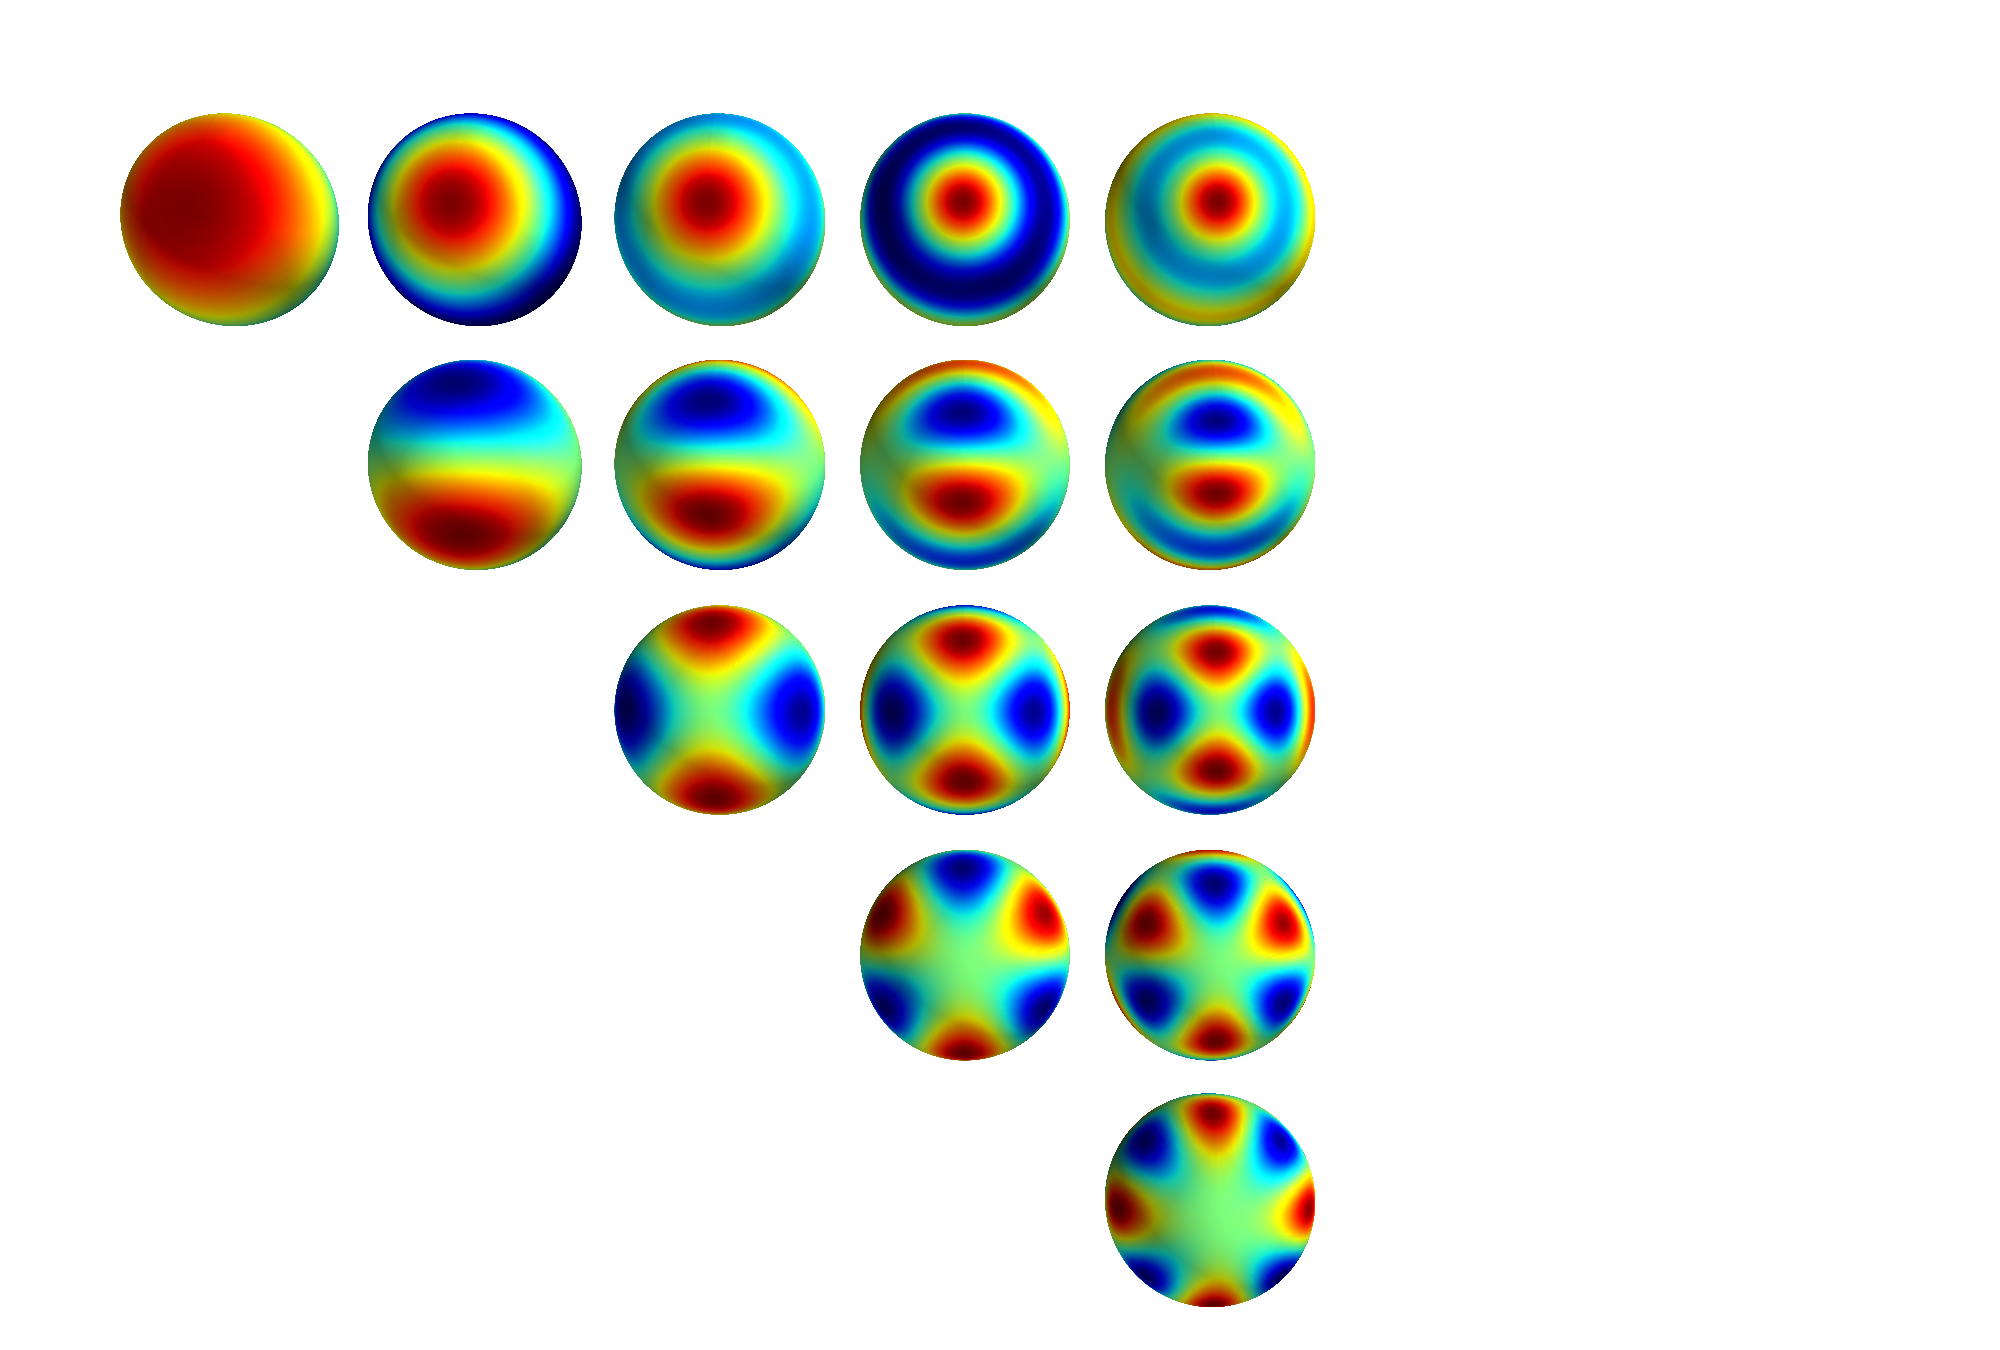
\includegraphics[width=\textwidth]{figures/spharmonics.png}
  \caption{Spherical Harmonics}
  \label{fig:spharmonics}
\end{figure*}

\begin{figure*}
  \centering
  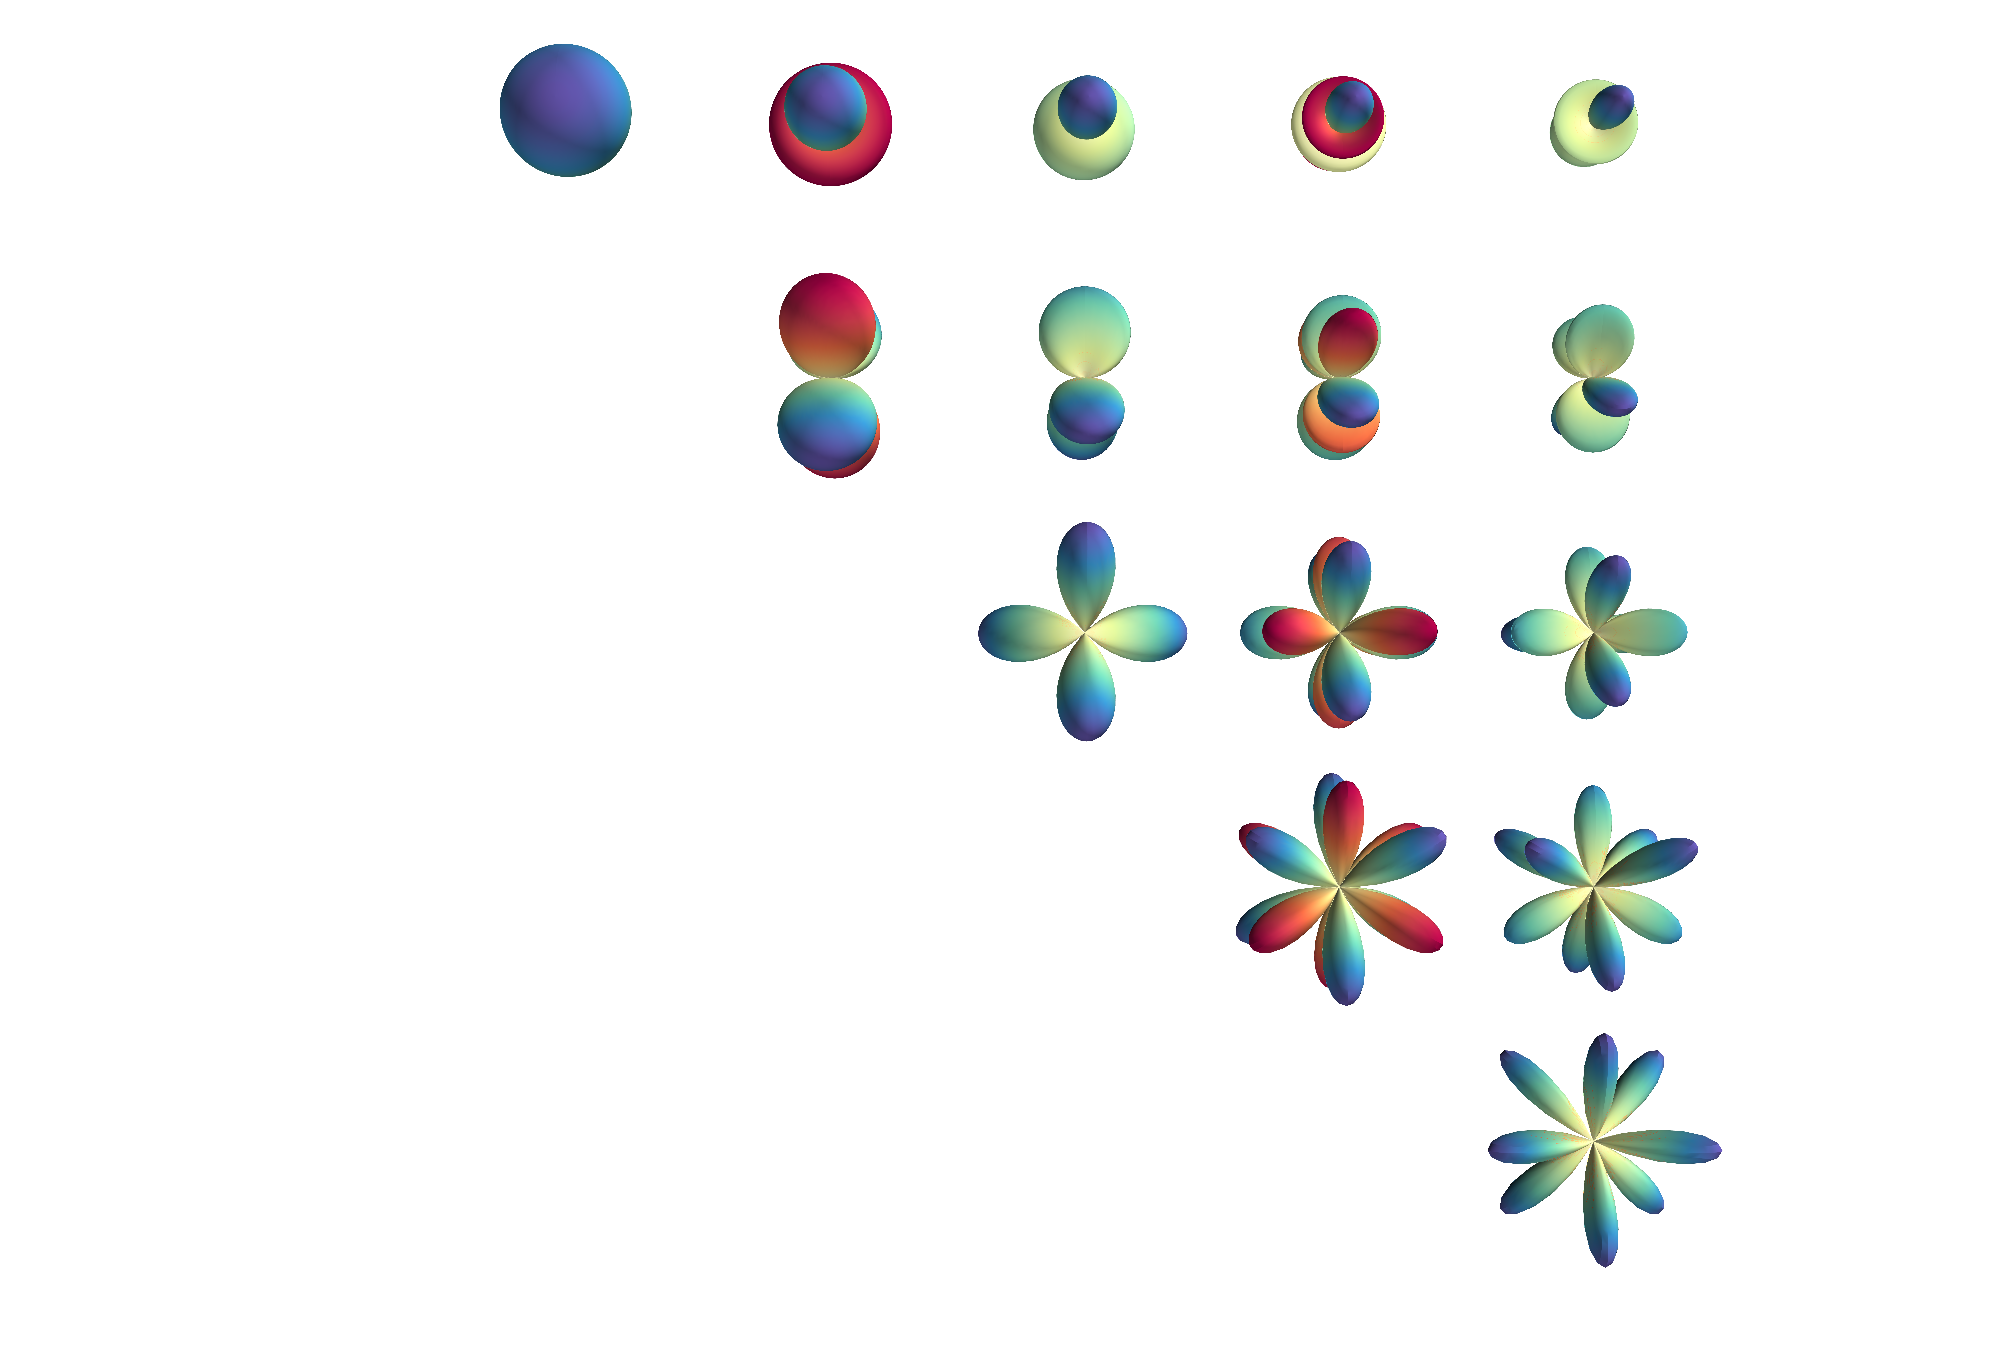
\includegraphics[width=\textwidth]{figures/spharmonics2.png}
  \caption{An alternative representation of Spherical Harmonics}
  \label{fig:spharmonics}
\end{figure*}

Spherical harmonics with a negative $m$ value can be related to those
with a positive $m$ value via
\begin{equation}
  \label{eq:negativespharm}
  Y_{l, -m} (\theta, \phi) = (-1)^m Y^{*}_{lm} (\theta, \phi)
\end{equation}
and they are orthogonal,
\begin{equation}
  \label{eq:spahrmorthog}
  \int \dd{\Omega} Y^{*}_{lm} (\theta, \phi) Y_{l^{\prime}m^{\prime}}(\theta, \phi) = \delta_{l l^{\prime}} \delta_{m, m^{\prime}}
\end{equation}
The first few spherical harmonics are
\[ Y_{00} = \sqrt{\frac{1}{4 \pi}} \]
\[ Y_{10}= \sqrt{\frac{3}{4 \pi}} \cos(\theta) \]
\[ Y_{1, \pm 1} = \mp \sqrt{\frac{3}{8 \pi}} \sin(\theta) e^{\pm i \phi} \]

\subsection{Spherical Harmonics and the Schrodinger Equation}
\label{sec:spherharmschrod}

In spherical coordinates the time-independent Schrodinger equation is
\begin{equation}
  \label{eq:tisespherical}
  \begin{split}
  - \frac{\hbar^2}{2m} \frac{1}{r^2 \sin^2 \theta} \bigg( \pdv{r} \qty[ r^2 \sin(\theta) \pdv{\psi}{r}] 
+ \pdv{\theta} \qty[ \sin \theta  \pdv{\psi}{\theta}] \\ + \pdv{\phi} \qty[ \frac{1}{\sin \theta} \pdv{\psi}{\phi}] \bigg) 
+ (V-E)\psi = 0
\end{split}
\end{equation}
Now, splitting this into the radial part and an angular part,
\begin{equation}
  \label{eq:sepschrod}
  \psi(r, \theta, \phi) = R(r) Y(\theta, \phi)
\end{equation}
Then, substituting this in, and setting both sides of the equation
equal to $l(l+1)$ we get two independent solutions
\begin{align}
  \dv{r} \qty[r^2 \dv[2]{R}{r}] - \frac{2m}{\hbar^2} \qty(V(r)-E) r^2
  R - l(l+1) R &= 0 \\\frac{1}{\sin \theta} \pdv{\theta} \qty[ \sin
  \theta \pdv{Y}{\theta}] + \frac{1}{\sin^2(\theta)}
  \pdv[2]{Y}{\phi} +l(l+1)Y &= 0
\end{align}
The angular part is solved by spherical harmonics,
\begin{equation}
  \label{eq:sphericalharmonics}
  Y_l^m(\theta, \phi) = N e^{im\phi} P_l^m (\cos \theta)
\end{equation}

\section{Bessel Functions}
\label{sec:bessel}

Bessel functions are the solutions to Bessel's differential equation,
\begin{equation}
  \label{eq:besselde}
  x^2 \dv[2]{y}{x} + x \dv{y}{x} + (x^2 - \alpha^2)y = 0
\end{equation}
with $p$ a constant. 

\subsection{Bessel functions from the Generating Function}
\label{sec:besselgen}

The Bessel functions can be described by a generating function,
\begin{equation}
  \label{eq:besselgen}
  g(x,t) = \exp(\frac{x}{2t}(t^2-1)) = \sum_{\nu=-\infty}^{\infty} J_{\nu}(x) t^{\nu}
\end{equation}

So, for Bessel functions of integer order we can expand this to form a series expansion,
\begin{equation}
  \label{eq:besselseriesexp}
  J_n(x) = \sum^{\infty}_{s=0} \frac{(-1)^s}{s! (n+s)!} \qty( \frac{x}{2} )^{n+2s} \approx \frac{x^n}{2^n n!}
\end{equation}
for small $x$.

Bessel functions with a negative index can be found from the relation
\begin{equation}
  \label{eq:negativebessel}
  J_{-\nu}(x) = (-1)^{\nu} J_{\nu}(x)
\end{equation}

\begin{figure}
  \centering
  \begin{tikzpicture}
    \begin{axis} [
    width=\linewidth, height=2in,
    xmin=0, xmax=20,
%   xtick={7700,7725,...,7800},
%   ymin=0.009, ymax=0.05,
    ]
    \addplot gnuplot[raw gnuplot, id=bess, mark=none, muted-blue, ultra thick]{
      set xrange[0:20];
      plot besj0(x);
    };
    \addplot gnuplot[raw gnuplot, id=bess2, mark=none, muted-green, ultra thick]{
      set xrange[0:20];
      plot besj1(x);
    };
    \addplot gnuplot[raw gnuplot, id=bess3, mark=none, muted-orange, ultra thick]{
      set xrange[0:20];
      fac(n) = (int(n)==0) ? 1.0 : int(n) * fac(int(n)-1.0);
      besj_eps = 0.1;
      besj(n,x) = (n==0) ? besj0(x) : (n==1) ? besj1(x) : (abs(x)<besj_eps*(n+1)) ? (x/2.0)**n/fac(n) : 2*(n-1)/x*besj(n-1,x) - besj(n-2,x);
      plot besj(2,x);
    };
    \addplot gnuplot[raw gnuplot, id=bess4, mark=none, accent-purple, ultra thick]{
      set xrange[0:20];
      fac(n) = (int(n)==0) ? 1.0 : int(n) * fac(int(n)-1.0);
      besj_eps = 0.1;
      besj(n,x) = (n==0) ? besj0(x) : (n==1) ? besj1(x) : (abs(x)<besj_eps*(n+1)) ? (x/2.0)**n/fac(n) : 2*(n-1)/x*besj(n-1,x) - besj(n-2,x);
      plot besj(3,x);
    };
    \addplot gnuplot[raw gnuplot, id=bess5, mark=none, accent-red, ultra thick]{
      set xrange[0:20];
      fac(n) = (int(n)==0) ? 1.0 : int(n) * fac(int(n)-1.0);
      besj_eps = 0.1;
      besj(n,x) = (n==0) ? besj0(x) : (n==1) ? besj1(x) : (abs(x)<besj_eps*(n+1)) ? (x/2.0)**n/fac(n) : 2*(n-1)/x*besj(n-1,x) - besj(n-2,x);
      plot besj(4,x);
    };

    % \addplot gnuplot [raw gnuplot, id=test, mark=none, color=blue]{
    %   set xrange[0:20];
    %   unset key;

    %   fac(n) = (int(n)==0) ? 1.0 : int(n) * fac(int(n)-1.0);
    %   besj_eps = 0.1;
    %   besj(n,x) = (n==0) ? besj0(x) : (n==1) ? besj1(x) : (abs(x)<besj_eps*(n+1)) ? (x/2.0)**n/fac(n) : 2*(n-1)/x*besj(n-1,x) - besj(n-2,x);

    %   plot besj0(x), besj1(x), besj(2,x), besj(3, x);
    % };

    \end{axis}
\end{tikzpicture}
  \caption{The first five Bessel functions}
  \label{fig:bessel}
\end{figure}

\subsection{Recurrence Relation for Bessel Functions}
\label{sec:besselrecu}
The Bessel functions can be descried by a pair of recurrence relations, found by differentiating with respect to $t$,

\begin{equation}
  \label{eq:recurrencebessel}
  J_{\nu-1}(x) + J_{\nu+1}(x) = \frac{2 \nu}{x} J_{\nu}(x)
\end{equation}
and by differentiating with respect to $x$,
\begin{equation}
  \label{eq:recurrencebessel2}
  J_{\nu-1}(x) - J_{\nu+1}(x) = 2J_{\nu}^{\prime}(x)
\end{equation}

A number of other integral relationships also exist.
\begin{align}
  \int x^n J_{n-1}(x) \dd{x} &= x^n J_n(x) \\
  \int x^{-n} J_{n+1}(x) \dd{x} &= -x^{-n} J_n(x) \\
  \int J_1(x) \dd{x} &= -J_0(x)
\end{align}

\subsection{Orthogonality of the Bessel Functions}
\label{sec:orthogonbessel}

The orthogonality relations for Bessel functions are similar to those
of the trigonometric functions, but they include an additional weighting factor, $r$.

\begin{equation}
  \label{eq:orthogbess}
  \int_0^a r J_p \qty( \frac{\alpha r}{a} ) J_p \qty(\frac{\beta r}{a}) \dd{r} = \delta_{\alpha \beta} \frac{a^2}{2} J_{p+1}^2(\alpha)
\end{equation}
with
\begin{align*}
  J_p(\alpha) = J_p(\beta) = 0
\end{align*}

\subsection{Bessel Series}
\label{sec:besselseries}

The orthogonality relations for Bessel functions allow the definition of Bessel series,
\begin{equation}
  \label{eq:besselser}
  f(x) = \sum_0^{\infty} c_n J_p(k_n x)
\end{equation}
with $J_p(k_na)=0$.

\begin{example}
  {\em Deriving the steady state inside an infinite cyclinder with the curved sides kept at a temperature $T_0$, and the base at $T_1$.}\\
  We know $\nabla^2 T =0$, and we can use seperation of variables to give a solution of the form $T = R(r)\Theta(\theta)Z(z)$.
  Then, in cylinderical coordinates,
  \begin{equation*}
    \frac{1}{R}\frac{1}{r} \dv{r} \qty(r \dv{R}{r}) + \frac{1}{\Theta} \frac{1}{r^2} \dv[2]{\Theta}{\theta} + \frac{1}{Z} \dv[2]{Z}{z} = 0
  \end{equation*}
We now have
\[ \frac{1}{Z} \dv[2]{Z}{z} = k^2 \]
implying
\[ Z = \exp(\pm kz) \]
also,
\[ \frac{1}{R}\frac{1}{r} \dv{r} \qty(r \dv{R}{r}) + \frac{1}{\Theta} \frac{1}{r^2} \dv[2]{\Theta}{\theta} + k^2 = 0 \]
which we can multiply by $r^2$,
\[ \frac{r}{R} \dv{r} \qty(r \dv{R}{r}) + \frac{1}{\Theta} \dv[2]{\Theta}{\theta} + k^2 r^2 = 0 \]
from which,
\[ \frac{1}{\Theta} \dv[2]{\Theta}{\theta} = -n^2 \]
implying that
\[ \Theta = \{ \cos(n \theta), \sin(n \theta) \} \]
and the periodicity of $\theta$ will force $n$ to be a natural number.
Then
\[ \frac{r}{R} \dv{r} \qty(r \dv{R}{r}) + (k^2 r^2 - n^2) = 0 \]
and letting $kr = s$,
\[ s \dv{s} \qty( s \dv{R}{s} ) + (s^2 - n^2)R = 0 \] which has the
form of Bessel's differential equation, equation (\ref{eq:besselde}),
and thus the solutions are Bessel functions, $J_n(s)$,
the complete solution is thus
\begin{equation*}
  J_n (kr) \qty( A \sin(n\theta) + B \cos(n \theta) ) e^{-kz}
\end{equation*}
We can ignore the Bessel functions which are infinite at $r=0$, as we
need a finite solution there, so the first-order functions are the
appropriate solutions.  We know that $T_1 > T_0$, so $T>T_0$
everywhere, and so $T_0$ can be taken as a constant. The boundary
condition of the curved surface at $r=a$ is where $J_n(ka) = 0$. We
now need to know the zeros of the Bessel functions, and our solution becomes
\begin{equation*}
  T = T_0 + \sum_{m=0}^{\infty} c_m J_0 \qty(\alpha_{0m}\frac{r}{a}) \exp(-\qty(\frac{\alpha_{0m}z}{a}))
\end{equation*}
The boundary condition at $z=0$ is that $T=T_0$, so
\[ T_1 - T_0 = \sum_m c_m J_0 \qty( \alpha_{0m} \frac{r}{a}) \]
and using the orthogonality condition,
\[ \int_0^a (T_1 - T_0) J_0 \qty( \alpha_{0m} \frac{r}{a} ) r \dd{r} = c_m \frac{a^2}{2} J_1^2(\alpha_{0m}) \]
and then, from the indefinite integral relationship $\int x J_0(x) \dd{x} = x J_1(x)$,
\begin{align*}
(T_1-T_0) \frac{a}{\alpha_{0m}} \qty[ r J_1 \qty( \alpha_{0m} \frac{r}{a})]_0^a &= (T_1 - T_0) \frac{a^2}{\alpha_{0m}} J_1 (\alpha_{0m})\\
&= c_m \frac{a^2}{2} J_1^2 (\alpha_{0m})
\end{align*}
with
\[ c_m = \frac{2}{\alpha_{0m}} \frac{1}{J_1(\alpha_{0m}} (T_1-T_0) \]
and the overarching solution is thus
\begin{equation*}
  T = T_0 + \sum_m \frac{2 (T_1-T_0)}{\alpha_{0m}J_1(\alpha_{0m})} J_0 \qty( \alpha_{0m} \frac{r}{a}) \exp( - \qty(\frac{\alpha_{0m}z}{a}) )
\end{equation*}
\end{example}

\subsection{Spherical Bessel Functions}
\label{sec:sphbess}

The spherical Bessel functions are a class of Bessel function related to the half-integer order order Bessel functions by
\begin{equation}
  \label{eq:sphericalbess}
  j_n(x) = \sqrt{\frac{\pi}{2x}} J_{n+\frac{1}{2}}(x) = x^n \qty(- \frac{1}{x} \dv{x})^n \frac{\sin(x)}{x}
\end{equation}
\begin{example}
{\em Finding energy levels of particles inside a spherical box using Schrodinger's equation.}\\
Starting at 
\[ - \frac{\hbar^2}{2m} \nabla^2 \Psi = E \Psi \]
after seperating variables
\[ \pdv{r} \qty(r^2 \pdv{R}{r}) + \qty( \frac{2mEr^2}{\hbar^2} - l(l+1) )R=0 \]
letting 
\[ k^2 = \frac{2mE}{\hbar^2} \quad \text{and} \quad s=kr\]
\[ s^2 \pdv[2]{R}{s} + 2s \pdv{R}{s} + \qty(s^2 - l(l+1))R = 0 \]
and letting
\[ R = \frac{Z}{s^{\frac{1}{2}}} \]
\[ s^2Z^{\prime \prime} + s Z^{\prime} + (s^2 - \qty(l + \frac{1}{2})^2 ) Z = 0 \]
Which is Bessel's equation of order $l+\half$, so
\[ R = j_l \qty( \frac{\sqrt{2mE}}{\hbar} r) \]
which is a finite solution as $r \to 0$.
The lowest energy state will have $l=0$ (so no angular variation), and to satisy the boundary condition of $R=0$ when $r=a$, we need
\[ j_0 \qty( \frac{\sqrt{2mE}}{\hbar}a)=0 \]
the zeros of $j_0$ are the same as those of $\sin(x)$, since
\[ j_0(x) = \frac{\sin(x)}{x} \]
so
\[ \frac{a \sqrt{2mE_{\rm min}}}{\hbar} = \pi \]
thus
\[ E_{\rm min} = \frac{\pi^2 \hbar^2}{2ma^2} \]
\end{example}
\section{Hermite Polynomials}
\label{sec:hermite}

\begin{figure}
  \centering
  \begin{tikzpicture}
    \begin{axis} [
    width=\linewidth, height=2in,
    xmin=-3, xmax=3,
    ymin=-60, ymax=50,
%   xtick={7700,7725,...,7800},
%   ymin=0.009, ymax=0.05,
    ]
    \addplot gnuplot[raw gnuplot, id=bess, mark=none, muted-blue, ultra thick]{
      set xrange[-3:3];
      set yrange[-40:50];	
      herm(n,x) = (n==0) ? 1 : (n==1) ? 2*x : 2*x*herm(n-1,x)-2*n*herm(n-2,x);
      plot herm(0,x);
    };
    \addplot gnuplot[raw gnuplot, id=bess2, mark=none, muted-green, ultra thick]{
      set xrange[-3:3];
      set yrange[-40:50];	
      herm(n,x) = (n==0) ? 1 : (n==1) ? 2*x : 2*x*herm(n-1,x)-2*n*herm(n-2,x);
      plot herm(1,x);
    };
    \addplot gnuplot[raw gnuplot, id=bess3, mark=none, muted-orange, ultra thick]{
      set xrange[-3:3];
      set yrange[-40:50];	
      herm(n,x) = (n==0) ? 1 : (n==1) ? 2*x : 2*x*herm(n-1,x)-2*n*herm(n-2,x);
      plot herm(2,x);
    };
    \addplot gnuplot[raw gnuplot, id=bess4, mark=none, accent-purple, ultra thick]{
      set xrange[-3:3];
      set yrange[-40:50];	
      herm(n,x) = (n==0) ? 1 : (n==1) ? 2*x : 2*x*herm(n-1,x)-2*n*herm(n-2,x);
      plot herm(3,x);
    };
    \addplot gnuplot[raw gnuplot, id=bess5, mark=none, accent-red, ultra thick]{
      set xrange[-3:3];
      set yrange[-40:50];	
      herm(n,x) = (n==0) ? 1 : (n==1) ? 2*x : 2*x*herm(n-1,x)-2*n*herm(n-2,x);
      plot herm(4,x);
    };
    \end{axis}
\end{tikzpicture}
  \caption{The first five Hermite Polynomials}
  \label{fig:hermite}
\end{figure}
Hermite polynomials are the solutions to the hermite equation,
\begin{equation}
  \label{eq:hermitede}
  \dv[2]{y}{x} - 2x \dv{y}{x} + 2n y = 0
\end{equation}
Hermite polynomials are solutions to the radial part of the
Schrodinger equation for the simple harmonic oscillator. Just like
Legendre polynomials and Bessel functions we can define Hermite
polynomials, $H_n (x)$ via a generating function:
\begin{equation}
  \label{eq:hermite}
  g(x,t) = e^{-t^2 + 2tx} = \sum^\infty_{n=0} H_n(x) \frac{t^n}{n!}
\end{equation}

\subsection{Recurrence Relations for Hermite polynomials}
\label{sec:hermiterecurs}

First we diferentiate with respect to $t$,
\[ \frac{\partial}{\partial t} g(x,t) = (-2t+2x) e^{-t^2+2tx} =
\sum^{\infty}_{n=1} H_n(x) \frac{t^{n-1}}{n!} \] Expanding, and
putting into the generating function again,
\[ -2 \sum^{\infty}_{n=0} H_n(x) \frac{t^{n+1}}{n!} + 2x
\sum^{\infty}_{n=0} H_n(x) \frac{t^n}{n!} = \sum^{\infty}_{n=1}
H_n(x)\frac{t^{n-1}}{(n-1)!} \]
Relabelling the indices,
\[ -2 \sum^{\infty}_{n=1} nH_{n-1}(x) \frac{t^{n}}{n!} + 2x
\sum^{\infty}_{n=0} H_n(x) \frac{t^n}{n!} = \sum^{\infty}_{n=1}
H_{n+1}(x)\frac{t^n}{n!} \]
and finally equating coefficients of $t^n$, 
\begin{equation}
  \label{eq:recurrencehermite}
  H_{n+1}(x) = 2x H_n(x) - 2n H_{n-1}(x) \qquad (n \ge 1)
\end{equation}
If we instead differentiate with respect to $x$,
\[ \pdv{x}g(x,t) = 2t e^{-t^2+2tx} = \sum_{n=0}^{\infty} H^{\prime}_n(x) \frac{t^n}{n!} \]
and substitute in $g$,
\[ 2 \sum_{n=0}^{\infty} H_n(x) \frac{t^{n+1}}{n!} = \sum_{n=1}^{\infty} H^{\prime}_n(x) \frac{t^n}{n!}\]
and relabelling,
\[ 2 \sum_{n=1}^{\infty} H_{n-1}(x) \frac{t^{n}}{(n-1)!} = \sum_{n=1}^{\infty} H^{\prime}_n(x) \frac{t^n}{n!}\]
and then equating coeffients of $t^n$,
\begin{equation}
  \label{eq:recurrencehermite2}
  H_n^{\prime}(x) = 2n H_{n-1}(x)
\end{equation}
These can be used to derive the ordinary differential equation which
motivates these polynomials,
from the previous results we can find
\[ H_{n+1}(x) = 2x H_n(x) - H^{\prime}_n(x) \]
and then differentiate with respect to $x$,
\begin{align*}
  H^{\prime}_{n+1}(x) &= 2 H_n(x) + 2x H^{\prime}_n(x) - H^{\prime \prime}_n(x) \\
  2(n+1)H_{n}(x) &= 2 H_n(x) + 2x H^{\prime}_n(x) - H^{\prime \prime}_n(x) 
\end{align*}
and so
\begin{equation*}
  \dv[2]{H_n(x)}{x} - 2x \dv{H_n(x)} + 2n H_n(x) = 0
\end{equation*}

It is possible to use the recurrence relations to find the Hermite polynomials,
so
\begin{align*}
  H_0(x) &=  1 \\
  H_1(x) &=  2x \\
  H_2(x) &=  4x^2 - 2 \\
  H_3(x) &=  8x^3 - 12x \\
  H_4(x) &=  16x^4 - 48x^2 + 12
\end{align*}

\subsection{Properties of the Hermite Polynomials}
\label{sec:hermiteprops}

The Hermite polynomials are symmetric about $x=0$, so
\begin{equation}
  \label{eq:parityhermite}
  H_n(-x) = (-1)^n H_n(x)
\end{equation}

The Hermite polynomials can be described by a specific series of the form
\begin{equation}
  \label{eq:hermiteseriesspef}
  H_n(x) = \sum_{m=0}^{\frac{n}{2}}(-1)^m (2x)^{n-2m} \frac{n!}{(n-2m)!m!}
\end{equation}

And Rodrigues's equation for Hermite polynomials also exists
{\em proof is an exercise}
\begin{equation}
  \label{eq:rodrigueshermite}
  H_n(x) = (-1)^n e^{x^2} \dv[n]{x} \qty(e^{-x^2})
\end{equation}

\subsection{Orthogonality of Hermite Polynomials}
\label{sec:orth-herm-polyn}

It is possible to show the orthogonality of the Hermite polynomials.
Starting at Hermite's equation,
\begin{align*}
  H_n^{\prime \prime}(x) - 2x H^\prime_n (x) + 2n H_n (x) &= 0 \\
\dv{x} \qty( e^{-x^2} \dv{x} H_n (x) ) + 2n e^{-x^2} H_n(x) &=0 
\end{align*}
then, proceeding in much the same way as with Legendre polynomials in
section \ref{sec:orthogonallegendre},
\begin{align*}
\begin{split}
  H_m(x) \dv{x} \qty[ e^{-x^2} \dv{x} H_n(x) ] - H_n(x) \dv{x} \qty[ e^{-x^2} \dv{x} H_m(x)] \\= -H_m(x) \cdot 2 n e^{-x^2} H_n(x) + H_n(x) \cdot 2 m e^{-x^2} H_m(x) 
\end{split}
\end{align*}
\begin{align*}
\begin{split}
\int_{-\infty}^{\infty} H_m(x) \dv{x} \qty[ e^{-x^2} \dv{x} H_n(x)] \dd{x} \\= \qty[ H_m(x) e^{-x^2} \dv{x} H_n(x)]_{-\infty}^{\infty} - \int_{-\infty}^{\infty} \qty[ \dv{x} H_m(x)] e^{-x^2} \dv{x} H_n(x) \dd{x}
\end{split}
\end{align*}
\begin{align*}
  2(m-n) \int_{-\infty}^{\infty} H_n(x) H_m(x) e^{-x^2} \dd{x} &= 0 \\
\therefore \int_{-\infty}^{\infty} H_n(x) H_m(x) e^{-x^2} \dd{x} &= 0 \text{ iff } n \neq m
\end{align*}
Hermite polynomials are orthogonal on the interval $[-\infty, \infty]$
with a weighting of $\exp(-x^2)$.
\begin{align*}
  \int_{-\infty}^{\infty} g^2(x,t) e^{(-x^2)} \dd{x} &= \int_{-\infty}^{\infty} \exp(-2t^2+4tx-x^2) \dd{x} \\
&= \sum_{n=0}^{\infty} \sum_{m=0}^{\infty} \frac{t^{n+m}}{n! m!} \int_{-\infty}^{\infty} H_n(x) H_m(x) e^{(-x^2)} \dd{x} \\
&= e^{2t^2}\int_{-\infty}^{\infty} e^{-x^2} \dd{x}\\
&= e^{2t^2} \sqrt{\pi} \\
&= \sqrt{\pi} \sum_{n=0}^{\infty} \frac{2^n}{n!} t^{2n}
\end{align*}
Finally, equating powers of $t^{2n}$ gives
\[ \int_{-\infty}^{\infty} \qty[ H_n(x)]^2 \exp(-x^2) = 2^n \sqrt{\pi} n! \]
so,
\begin{equation}
\label{eq:hermiteorthoweight}
\int_{-\infty}^{\infty} H_n(x) H_m(x) \exp(-x^2) \dd{x} = 2^n \sqrt{\pi} n! \delta_{nm}
\end{equation}
it is also possible to remove the weighting by redefining the polynomial as
\[ \phi_n(x) := \exp(-x^2) H_n(x) \]
in this case
\begin{equation}
  \label{eq:hermiteorthonoweight}
  \int_{-\infty}^{\infty} \phi_n(x) \phi_m(x) \dd{x} = 2^n \sqrt{\pi} n! \delta_{nm}
\end{equation}
these, however, are solutions not of Hermite's equation, but of a slightly variant equation,
\begin{equation}
  \label{eq:modhermiteequation}
  \phi^{\prime \prime}_n(x) + (1-x^2+2n) \phi_n(x) = 0 
\end{equation}

\subsection{The Quantum Harmonic Oscillator}
\label{sec:quant-harm-oscill}

Returning to the one-dimensional time-independent Schr\"odinger
equation,
\begin{equation}
  \label{eq:1}
  - \frac{\hbar^2}{2m} \dv[2]{x} \psi(x) + V(x) \psi(x) = E \psi(x)
\end{equation}
with $m$ the mass of the particle, and $E$ its energy. For the simple harmonic oscillator, 
\[ V(x) \half m \omega^2 x^2 \]
so
\[ \psi^{\prime \prime} (x) + \qty( - \frac{m^2 \omega^2}{\hbar^2} x^2
+ \frac{2m E}{\hbar^2} ) \psi(x) = 0 \] which has a form very similar
to the modified Hermite equation of the previous section, and these
describe the quantum harmonic oscillator.

Let $y = ax$ with $a = \sqrt{\frac{m \omega}{\hbar}}$, so
\[ \dv[2]{\psi}{y} + \qty( -y^2 + \frac{2mE}{\hbar^2 a^2} ) \psi =
0 \]
Comparing the two equations, we get the solutions
\begin{equation}
  \label{eq:2}
  \psi_n (x) = \sqrt{\frac{a}{2^n \sqrt{\pi} n!}} \exp( - \frac{a^2 x^2}{2} ) H_n(ax) 
\end{equation}
which includes a normalisation constant. The energy is then given by the equation
\begin{align}
  \frac{2 m E}{\hbar^2 a^2} &= 1 + 2n \nonumber\\
\frac{2E}{\hbar \omega} &= 1 + 2n \nonumber\\
E &= \hbar \omega \qty(n + \half)
\end{align}
but why does $n$ need to be an integer? The oscillator must have $\Psi
\to 0$ as $x \to \infty$. Taking solutions of the form
\[ \Psi \approx \exp( - \frac{x^2}{2} ) H_n(x) \] only guarantees this
if $n$ is an integer; this can be demonstrated by returning to
Hermite's equation, equation (\ref{eq:hermitede}), and letting $y =
\sum_{k=0}^{\infty} c_k x^k$, so that
\[ \sum_k c_k \qty( k(k-1) x^{k-2} - 2kx^k + 2nx^k ) = 0 \]
This must be true for each power of $x$ individually, so
\[ c_{k+2} (k+2) (k+1) - c_k(2k-2n)=0 \]
and if the series in $k$ goes on \emph{ad infinitum}, we have the behaviour
\begin{equation*}
  \frac{c_{k+2}}{c_k} = \frac{2k - 2n}{(k+1)(k+2)} \to \frac{2}{k} \quad \text{as} \quad k \to \infty
\end{equation*}
This has the power series behaviour of $\exp(x^2)$, which would imply
that $\Psi \approx e^{x^2} e^{-\frac{x^2}{2}} \approx
e^{\frac{x^2}{2}}$, giving ``bad'' behaviour as $x \to \infty$.  If
the series truncates this behaviour will not occur. This happens if
$2n=2k$ for some $k$, that is, for $n \in \mathbb{Z}$. The solution of
Hermite's equation is a finite polynomial, and the solution for $\Psi$
must be physical, so this forces $n$ to be an integer.

The harmonic oscillator can also be solved using ladder operators,
these work due to the recurrence relation in equation
(\ref{eq:recurrencehermite2}). Writing 
\[ \psi_n(x) = \sqrt{\frac{1}{2^n \sqrt{\pi} n!}} \exp( - \frac{x^2}{2} ) H_n(x) \]
and, for simplicity, letting $a=1$, then
\begin{align*}
 \frac{1}{\sqrt{2}} \qty(x + \dv{x}) \psi_n(x) &= \sqrt{\frac{1}{2^{n+1} \sqrt{\pi} n!}} \qty( x+ \dv{x}) \exp(- \frac{x^2}{2}) H_n(x) \\
%&= \sqrt{\frac{1}{2^{n+1} \sqrt{\pi} n!}} \qty( x \exp( - \frac{x^2}{2} ) H_n(x) - x \exp( - \frac{x^2}{2} ) H_n(x) + \exp( - \frac{x^2}{2}) H^{\prime}_n(x) ) 
\\ & = \sqrt{n} \psi_{n-1}(x)
\end{align*}
This is a lowering operator, it is also possible, using either recurrence relations or the Rodrigues' formula, that
\[ \frac{1}{\sqrt{2}} \qty( x - \dv{x} ) \] is a raising operator.

\section{Laguerre Polynomials}
\label{sec:laguerre}
The Laguerre polynomials are the solutions to the Laguerre equation,
\begin{equation}
  \label{eq:laguerrede}
  x L_n^{\prime \prime} (x) + (1-x) L_n^{\prime}(x) + n L_n(x) = 0
\end{equation}
The Laguerre polynomials are generated by the function
\begin{equation}
  \label{eq:3}
  g(x,t) = \frac{\exp( - \frac{xt}{(1-t)})}{1-t} = \sum_{n=0}^{\infty} L_n(x) t^n
\end{equation}

\subsection{Recurrence Relations }
\label{sec:recurr-relat-lag}

\begin{equation}
  \label{eq:4}
  (n+1) L_{n+1}(x) = (2n +1 -x) L_n(x) - nL_{n-1}(x)
\end{equation}

\begin{equation}
  \label{eq:5}
  xL^{\prime}_n(x) = nL_n(x) - nL_{n-1}(x)
\end{equation}

It is possible to use these recurrence relations to find the first few
Laguerre polynomials,
\begin{align*}
  L_0(x) &= 1 \\
L_1(x) &= 1-x \\
L_2(x) &= \half \qty(x^2 - 4x + 2)
\end{align*}

\subsection{Orthogonality}
\label{sec:orthogonality}

Using similar techniques as for other special functions, it can be demonstrated that
\begin{equation}
  \label{eq:orthoglag}
  \int_0^{\infty} L_n(x) L_m(x) \exp(-x) \dd{x} = \delta_{nm}
\end{equation}

\subsection{Properties}
\label{sec:properties}

The Laguerre polynomials have a Rodrigues' formula
\begin{equation}
  \label{eq:rodrigueslag}
  L_n(x) = \frac{e^x}{n!} \dv[n]{x} \qty(x^n e^{-x} )
\end{equation}
and a series expansion
\begin{equation}
  \label{eq:serieslag}
  L_n(x) = \sum_{s=0}^n (-1)^{n-s} \frac{n! x^{n-s}}{(n-s)!(n-s)!s!}
\end{equation}

\subsection{Associate Laguerre Polynomials}
\label{sec:assoc-lagu-polyn}

The associate Laguerre polynomials are solutions to the associate
Laguerre equation,
\begin{equation}
  \label{eq:assoclag}
  x y^{\prime \prime} (x) + (k+1-x) L_n^{k \prime}(x) + nL_n^k(x) = 0
\end{equation}
and are derived from the Laguerre polynomials by the expression
\begin{equation}
  \label{eq:assoclagfromlag}
  L_n^k(x) = (-1)^n \dv[k]{x} L_{n+k}(x)
\end{equation}
They are also orthogonal, with
\begin{equation}
  \label{eq:assoclagortho}
  \int_0^{\infty} L_n^k(x) L_m^k(x) x^k \exp(-x) \dd{x} = \frac{(n+k)!}{n!} \delta_{nm}
\end{equation}

\begin{example}{\em 3D Quantum Harmonic Oscillator}
  Consider a quantum harmonic oscillator with a potential
  \[ V = \half m \omega^2 \qty(x^2+y^2+z^2) = \half m \omega^2 r^2 \]
  First separating Schr\"odinger's equation into cartesian coordinates
  and then deriving the form of the wavefunction leads to the
  conclusion that the energies are quantised as
  \[ E = \qty( n+ \frac{3}{2}) \hbar \omega \] for $n = n_x + n_y +
  n_z$.  Separating Schr\"odinger into spherical coordinates allows
  the solutions to take the form
  \[ \Psi = N r^l \exp( - \half \alpha r^2) L_{\half(n-l)}^{l+\half}
  (\alpha^2 r^2) Y_{lm}(\theta, \phi) \] for \[ a = \sqrt{\frac{m
      \omega}{\hbar}} \] With $n$ a normalisation factor, and $l$
  taking the values $n, n-2, \dots, 0$.  Associated Laguerre
  polynomials with non-integer $p$ are obtained.
\end{example}

\begin{figure}
  \centering
  \begin{tikzpicture}
	\foreach \k in {0,1,2,3,4}{
	\begin{scope}[yshift=-1.8in*\k]
    \begin{axis} [
    title={$k=\k$},
    width=\linewidth, height=2in,
    xmin=0, xmax=5,
    ymin=-3, ymax=5
    ]
    \addplot gnuplot[raw gnuplot, id=alag, mark=none, muted-blue, ultra thick]{
      set xrange[-1:5];
      %set yrange[0:10];	
      lag(n,x) = (n==0) ? 1 : (n==1) ? -x+1 : ( (2*(n-1)+1-x) * lag(n-1,x) - (n-1) * lag(n-2, x) ) / (n);
      alag(n,k,x) = (k==0) ? lag(n,x) : ( (n+k)*alag(n, k-1, x) - (n+1)* alag(n+1, k-1, x) ) /x;
      plot alag(0,\k,x);
    };
    \addplot gnuplot[raw gnuplot, id=alag, mark=none, muted-green, ultra thick]{
      set xrange[-1:5];
      %set yrange[0:10];	
      lag(n,x) = (n==0) ? 1 : (n==1) ? -x+1 : ( (2*(n-1)+1-x) * lag(n-1,x) - (n-1) * lag(n-2, x) ) / (n);
      alag(n,k,x) = (k==0) ? lag(n,x) : ( (n+k)*alag(n, k-1, x) - (n+1)* alag(n+1, k-1, x) ) /x;
      plot alag(\k+1,\k,x);
    };
    \addplot gnuplot[raw gnuplot, id=alag, mark=none, muted-orange, ultra thick]{
      set xrange[-1:5];
      %set yrange[0:10];	
      lag(n,x) = (n==0) ? 1 : (n==1) ? -x+1 : ( (2*(n-1)+1-x) * lag(n-1,x) - (n-1) * lag(n-2, x) ) / (n);
      alag(n,k,x) = (k==0) ? lag(n,x) : ( (n+k)*alag(n, k-1, x) - (n+1)* alag(n+1, k-1, x) ) /x;
      plot alag(\k+2,\k,x);
    };
    \addplot gnuplot[raw gnuplot, id=alag, mark=none, accent-purple, ultra thick]{
      set xrange[-1:5];
      %set yrange[0:10];	
      lag(n,x) = (n==0) ? 1 : (n==1) ? -x+1 : ( (2*(n-1)+1-x) * lag(n-1,x) - (n-1) * lag(n-2, x) ) / (n);
      alag(n,k,x) = (k==0) ? lag(n,x) : ( (n+k)*alag(n, k-1, x) - (n+1)* alag(n+1, k-1, x) ) /x;
      plot alag(\k+3,\k,x);
    };
    \addplot gnuplot[raw gnuplot, id=alag, mark=none, accent-red, ultra thick]{
      set xrange[-1:5];
      %set yrange[0:10];	
      lag(n,x) = (n==0) ? 1 : (n==1) ? -x+1 : ( (2*(n-1)+1-x) * lag(n-1,x) - (n-1) * lag(n-2, x) ) / (n);
      alag(n,k,x) = (k==0) ? lag(n,x) : ( (n+k)*alag(n, k-1, x) - (n+1)* alag(n+1, k-1, x) ) /x;
      plot alag(\k+4,\k,x);
    };
    \end{axis}
\end{scope}
}
\end{tikzpicture}
  \caption{The Associate Laguerre Polynomials}
\end{figure}

% \subsubsection{Ladder Operators}
% \label{sec:ladder}

% We have a number of equally-spaced energy levels. Ladder operators
% move around these energy levels.
%%% Local Variables: 
%%% mode: latex
%%% TeX-master: "notes"
%%% End: 


\chapter{Linear Algebra}
\label{cha:linear-algebra}

\section{Fields of Scalars}
\label{sec:scalarfields}

A field is an algebraic structure with notions of addition,
subtraction, multiplication, and division, satisfying certain
axioms. The principle examples are $\mathbb{Q}$, $\mathbb{R}$, and
$\mathbb{C}$.

 \begin{definition}[Field of Scalars]
   A field of scalars consists of a set, $F$, whose elements are
   called scalars, together with two algebraic
   operations---addition and multiplication---for combining every
   pair of scalars, $x, y \in F$ to form the new scalars $(x+y) \in
   F$ and $(x \times y) \in F$.  These operations must satisfy the
  field axioms:
  \begin{enumerate}
  \item {\em Associativity}: For $x,y,z \in F$,
    \begin{align*}
      (x+y)+ z &= x+(y+z) \\
      (x\times y)\times z &= x \times (y \times z)
    \end{align*}
  \item {\em Distributivity}:
    \begin{align*}
      (x+y) \times z &= x \times z + y \times z \\
      z \times (x + y) &= z \times x + z \times y
    \end{align*}
  \item {\em Commutativity}:
    \begin{align*}
      x + y &= y + x \\
      x \times y &= y \times x
    \end{align*}
  \item {\em Zero and Unity}: There are unique and distinct
    elements, $0, 1 \in F$, such that
    \begin{align*}
      x+0 &= x = 0 + x \\
      x \times 1 &= x = 1 \times x
    \end{align*}
  \item {\em Additive and multiplicative inverses}: For $x \in F$
    there exists a unique element $-x \in F$, for which
    \[ x + (-x) = 0 = (-x)+x \] For each non-zero $y \in F$ there
    is a unique element $y^{-1} \in F$ for which \[ y \times
    (y^{-1}) = 1 = (y^{-1})\times y \]
  \end{enumerate}
 \end{definition}

\section{Vector Spaces}
\label{sec:vectorspace}

\begin{definition}[Vector Space]
  A vector space over $F$ is a set, $\vs{V}$ of elements called vectors on which addition, $\vec{u}+\vec{v}$ of vectors $\vec{u}$ and $\vec{v}$, is defined, scalar multiplication, $\lambda \vec{u}$ of a vector $\vec{u}$ by a scalar $\lambda$ from $F$ is defined and the following axioms hold:\\
\begin{subequations}
  \begin{align}
     \vec{u}+\vec{v} &\in \vs{V} \\
     (\vec{u} + \vec{v}) + \vec{w} &= \vec{u}+(\vec{v}+\vec{w}) \\
     \vec{u}+\vec{v} &= \vec{v}+\vec{u} \\
     \exists \vec{0} \in \vs{V} & \mid \vec{u}+\vec{0} = \vec{u}=\vec{0}+\vec{u} \\
     \forall \vec{u} \in \vs{V} \exists - \vec{u}\in \vs{V} & \mid \vec{u}+(-\vec{u}) = \vec{0} = (-\vec{u})+\vec{u} \\
     \lambda \vec{u} \in \vs{V} \\
     \forall \vec{u}, \vec{v} \in \vs{V} , \forall \lambda, \mu \in F, & \lambda(\vec{u}+\vec{v}) = \lambda \vec{u}+\lambda \vec{v}
  \end{align}
\end{subequations}
\end{definition}
\begin{definition}[Vector Subspace]
  A non-empty subset, $w$, of a vector space $\mathsf{V}$ over $F$, such that
  \begin{subequations}
    \begin{equation}
      \label{eq:subspaceaddclose}
      \vec{w}_1 + \vec{w}_2 \in w \qquad \forall \vec{w}_{1,2} \in w
    \end{equation}
    \begin{equation}
      \label{eq:scalarmultsubsclose}
      \lambda \vec{w} \in w \qquad \forall \vec{w} \in w, \forall \lambda \in F
    \end{equation}
  \end{subequations}
\end{definition}
\begin{definition}[Vector space sum]
  Let $\vs{U}_1$ and $\vs{U}_2$ be subspaces of a vector space $\vs{V}$, then the sum, $\vs{U}_1 + \vs{U}_2$ is defined,
  \begin{equation}
    \label{eq:vectorspacesum}
    \vs{U}_1 + \vs{U}_2 = \left\{ \vec{u}_1 + \vec{u}_2 \in \vs{V} \mid \vec{u}_1 \in \vs{U}_1 \wedge \vec{u}_2 \in \vs{U}_2 \right\}
  \end{equation}
i.e.\ $\vs{U}_1 + \vs{U}_2$ is the set of vectors in $\vs{V}$, that, expressed as a vector in $\vs{U}_1$ added to a vector in $\vs{U}_2$.
\end{definition}
\begin{definition}[Vector Direct Sum]
  A sum $\vs{U}_1 + \vs{U}_2$ in which every element can be expressed uniquely in the form $\vec{u}_1 + \vec{u}_2$, with $\vec{u}_1 \in \vs{U}_1$, and $\vec{u}_2 \in \vs{U}_2$ is called a direct sum, and is denoted
\[ \vs{U}_1 \oplus \vs{U}_2 \]
\end{definition}
\begin{lemma}
  The sum $\vec{u}_1 + \vec{u}_2$ is the direct sum, $\vec{u}_1 \oplus \vec{u}_2$ iff $\vec{u}_1 \cap \vec{u}_2 = \{\vec{0}\}$
\end{lemma}
\begin{definition}[Linear Combination]
  Let $\vec{u}_1, \vec{u}_2, \dots, \vec{u}_n$ be vectors in the vector space $\vs{V}$ over the field $F$. A linear combination of these vectors is a vector of the form
\[ \lambda_1 \vec{u}_1 + \lambda_2 \vec{u}_2 + \cdots + \lambda_n \vec{u}_n \]
with $\lambda_1, \lambda_2, \dots, \lambda_n \in F$.
\end{definition}
\begin{definition}[Span of a vector space]
   Let $\vec{u}_1, \vec{u}_2, \dots, \vec{u}_n$ be vectors in the vector space $\vs{V}$ over the field $F$,
then the subspace of $\vs{V}$ spanned by these vectors is denoted 
\[ {\rm sp}(\vec{u}_1, \vec{u}_2, \dots, \vec{u}_n) \]
and is defined by
\[ \left\{ \lambda_1 \vec{u}_1 + \lambda_2 \vec{u}_2 + \cdots +
  \lambda_n \vec{u}_n \mid \lambda_1, \lambda_2, \dots, \lambda_n \in
  F \right\} \] So the supspace spanned by this sequence of vectors is
the set of all linear combinations which may be formed from the
sequence.
\end{definition}
\begin{definition}[Finite Dimensional Vector Space]
  A finite dimensional vector space is one which is spanned by a
  finite sequence of vectors.
\end{definition}
\begin{definition}[Linearly Independent Sequence]
  A sequence of vectors $\vec{u}_1, \vec{u}_2, \dots, \vec{u}_n \in
  \vs{V}$ is called a linearly independent sequence iff
  \[ \lambda_1 \vec{u}_1 + \lambda_2 \vec{u}_2 + dots + \lambda_n
  \vec{u}_n = \vec{0}\] is only possible when
  \[ \lambda_1 + \lambda_2 + \cdots +\lambda_n = 0 \] with $\lambda_1,
  \lambda_2, \dots , \lambda_n \in F$.
\end{definition}
\begin{theorem}
  If $\vs{W}$ is a subspace of $\vs{V}$ such that it is spanned by
  $\vec{u}_1, \vec{u}_2, \dots, \vec{u}_n$, then there is a subspace
  of this sequence which is linearly independent and still spans
  $\vs{W}$.
\end{theorem}
\begin{definition}[Basis]
  A basis is a linearly independent sequence of vectors which is a
  span of a vector space.
\end{definition}
\begin{lemma}[Expressing elements in a vector space]
  Suppose $\vec{u}_1, \vec{u}_2, \dots, \vec{u}_n$ is a basis of
  \vs{V}. Then every element can be uniquely expressed as a linear
  combination of the sequence. The unique scalar multiples of each are the \emph{components} of the element $\vec{x} \in \vs{V}$.
\end{lemma}
\begin{theorem}
  Suppose $\vs{V}$ has a basis $\vec{u}_1, \vec{u}_2 \dots
  \vec{u}_n$. Then any sequence of vectors $\vec{w}_1, \vec{w}_2,
  \dots \vec{w}_m \in \vs{V}$ with $m > n$ is linearly dependent.
\end{theorem}
\begin{definition}[Dimension of a vector space]
  Suppose $\vs{V}$ is finite dimensional. Then the dimension of $\vs{V}$, denoted $\dim(\vs{V})$, is the number of vectors in any basis of $\vs{V}$.
\end{definition}
\begin{lemma}[Conditions for a basis]
  A sequence of vectors in $\vs{V}$ is a basis provided it possesses any two of the following conditions,
  \begin{enumerate}
  \item the sequence spans $\vs{V}$
  \item the sequence is linearly independent
  \item $n = \dim(\vs{V})$
  \end{enumerate}
\end{lemma}
\begin{lemma}[Properties of a vector subspace]
  Suppose $\vs{V}$ is finite dimensional; let $\vs{W}$ be a subspace of $\vs{V}$, then,
  \begin{enumerate}
  \item $\vs{W}$ is finite dimensional
  \item $\dim(\vs{W}) \leq \dim(\vs{V})$
  \item If $\vs{W} \neq \vs{V}$ then $\dim(\vs{W}) < \dim(\vs{V})$
  \item Any basis of $\vs{W}$ can be extended to be a basis of
    $\vs{V}$.
  \end{enumerate}
\end{lemma}

\subsection{Inner Product Spaces}
\label{sec:innerproduct}
In this section, let $\vs{V}$ denote a vector space over the field
$\mathbb{R}$, let $\vec{u}, \vec{v},$ and $\vec{w}$ be vectors from
$\vs{V}$, and $a, b, c,$ and $d$ be scalars from the field
$\mathbb{R}$.
\begin{definition}[Real Inner Product]
  Suppose to each pair of vectors $\vec{u},\vec{v} \in \vs{V}$ there
  is assigned a real number, denoted $\langle \vec{u}, \vec{v}
  \rangle$, which is called the real inner product on $\vs{V}$ if it
  satisfies the axioms
  \begin{enumerate}
  \item (Linearity)
    \[ \langle a \vec{u}_1 + b \vec{u}_2 , \vec{v} \rangle = a \langle
    \vec{u}_1, v \rangle + b \langle \vec{u}_2, \vec{v} \rangle \]
  \item (Symmetry)
    \[ \langle \vec{u}, \vec{v} \rangle = \langle \vec{v}, \vec{u}
    \rangle \]
  \item (positive definite)
    \[ \langle \vec{u}, \vec{u} \rangle \geq 0 \text{ and }
       \langle \vec{u}, \vec{u} \rangle = 0 \text{ iff } \vec{u} = 0. 
    \]
  \end{enumerate}
\end{definition}
\begin{definition}[Real Inner Product Space]
  A vector space, $\vs{V}$ on which a real inner product is defined is
  called a real inner product space.
\end{definition}
\begin{definition}[Norm of a vector]
  The third axiom of the inner product requires that it always be
  positive. This allows the definition of the norm,
  \[ ||\vec{u}|| = \sqrt{ \langle \vec{u}, \vec{u} \rangle } \] which
  is a measure of the length of the vector.
\end{definition}
There are numerous examples of inner product spaces, from Euclidean $n$-spaces (perhaps the most day-to-day example), function and polynomial space, matrix space, and Hilbert space.
\begin{theorem}[Cauchy-Schwarz Inequality]
  For any vectors $\vec{u}$ and $\vec{v}$ in an inner product space $\vs{V}$, 
  \[ \langle \vec{u}, \vec{v} \rangle^2 \leq \langle \vec{u}, \vec{u}
  \rangle \langle \vec{v}, \vec{v} \rangle \quad \text{or} \quad |
  \langle \vec{u}, \vec{v} \rangle \leq ||\vec{u}|| ||\vec{v}|| \]
\end{theorem}
\begin{theorem}[Properties of the Norm]
  Let $\vs{V}$ be an inner product space. Then the norm in $\vs{V}$ satisfies the following properties
  \begin{enumerate}
  \item $||\vec{v}|| \geq 0$ and $||\vec{v}||=0$ if and only if
    $\vec{v}=0$.
  \item $||k \vec{v}|| = |k| ||\vec{v}||$
  \item $||\vec{u} + \vec{v}|| \leq ||\vec{u}|| + ||\vec{v}||$
  \end{enumerate}
\end{theorem}
\begin{definition}[Orthogonal Vectors]
  Two vectors, $\vec{u}, \vec{v} \in \vs{V}$ are orthogonal iff
  \[ \langle \vec{u}, \vec{v} \rangle = 0 \]
\end{definition}
\begin{definition}[Orthonormal Vectors]
  Two vectors, $\vec{u}, \vec{v} \in \vs{V}$ are orthonormal iff
  \[ \langle \vec{u}_i, \vec{u}_j \rangle =
  \begin{cases}
    0 & \vec{u} \neq \vec{v} \\
    1 & \vec{u} = \vec{v}
  \end{cases}
  \]
\end{definition}
It follows that a sequence of orthogonal or orthonormal vectors is
linearly independent, and so can form a basis. In order to
orthogonalise a basis use the Gram-Schmidt Process.  Let $\vec{u}_1,
\vec{u}_2$ be linearly independent vectors with an angle $\theta$
between them. Then
\[ \theta = \frac{\langle \vec{u}_1, \vec{u}_2 \rangle}{||\vec{u}_1||
  || \vec{u}_2||} \] so $\vec{u}_2$ can be expressed as the sum of two
vectors in the direction of $\vec{v}_2$ (a new, vector orthogonal to
$\vec{u}_1$, and $\vec{u}_1$. For convenience, let $\vec{v}_1 = \vec{u}_1$.

\begin{algorithm}[Gram-Schmidt Process]
  For a sequence of non-orthonormal, linearly independent vectors
  $\vec{u}_1, \vec{u}_2, \dots, \vec{u}_n$, in order to produce an
  orthonormal sequence, $\vec{v}_1, \vec{v}_2, \dots, \vec{v}_n$,
  \begin{enumerate}
  \item Let $\vec{v}_1$
  \item Set 
\[\vec{v}_k = \vec{u}_k - \sum_{i=1}^{k-1} \frac{\langle \vec{v}_i, \vec{u}_k \rangle}{\langle \vec{v}_i, \vec{u}_i \rangle} \cdot \vec{v}_i \]
$\forall k \in \{ 1, ..., n \}$.
\item Normalise each vector by \[ \hat{v}_i = \frac{\vec{v}_i}{||\vec{v}_i||} \]
  \end{enumerate}
\end{algorithm}
\begin{definition}[Complex inner product spaces]
  Let $\vs{V}$ be a vector space over $\mathbb{C}$. Suppose each pair of vectors 
\end{definition}
\section{Matrices}
\label{sec:matrixtheory}

\begin{definition}[Matrix]
  A matrix, $A$ over a field $K$ is a rectangular, $n \times m$, array of scalars, which is usually represented in the form
\[ A =
\begin{pmatrix}
  a_{11} & a_{12} & \cdots & a_{1n} \\
  a_{21} & a_{22} & \cdots & a_{2n} \\
  \vdots & \vdots & \ddots & \vdots \\
  a_{m1} & a_{m2} & \cdots & a_{mn}
\end{pmatrix}
\]
Both the operations of addition and multiplication are defined for matrices.
\end{definition}
\begin{definition}[Main Diagonal]
  The main diagonal of a matrix are the entries $a_{ij}$ where $j=i$.
\end{definition}
\begin{definition}[Square Matrix]
  A matrix is called a square matrix if it is of shape $(n \times n)$.
\end{definition}

\begin{definition}[Upper and Lower Triangular Matrices]
  If a square matrix has only zeros below every entry in the main
  diagonal it is an upper triangular matrix. If the matrix has only
  zeros above every entry in the main diagonal it is lower triangular.
\end{definition}

\begin{definition}[Diagonal Matrix]
  A matrix is called diagonal if all of the entries lying off the main
  diagonal are zero. A diagonal matrix may also be written as 
  \[ \operatorname{diag}(a_{11}, a_{22}, \cdots, a_{nn}) \]
\end{definition}
It should be noted that a diagonal matrix is both upper and lower
triangular.

\begin{definition}[Cofactors of a  Matrix]
  The cofactors, $A^{ij}$ of an $n \times n$ matrix $A$ is the
  $(n-1) \times (n-1)$ matrix containing the elements of $A$ excluding
  those in the $i^{\rm th}$ row and the $j^{\rm th}$ column.
\end{definition}

\begin{definition}[Cofactor Matrix]
  A cofactor matrix is a matrix whose elements are all cofactors, and has the form
\[ C = 
\begin{pmatrix}
  C_{11} & C_{12} & \cdots & C_{1n} \\
  C_{21} & C_{22} & \cdots & C_{2n} \\
  \vdots & \vdots & \ddots & \vdots \\
  C_{n1} & C_{n2} & \cdots & C_{nn}
\end{pmatrix}
\]
\end{definition}

\subsubsection{Matrix Operations}
\label{sec:matops}

\begin{definition}[Matrix Transpose]
  The transpose of a square matrix $A$ is defined
  \[ \qty[\trans{A}]_{ij} = \qty[A]_{ji} \] that is, the transpose of
  a matrix is the original matrix reflected about its main diagonal.
\end{definition}

\begin{definition}[Matrix Trace]
  The trace of a square matrix, $A$ is the sum of the elements in its main diagonal, ie.\
  \[ \trace(A) = \sum^n_{i=1} a_{ii}\] where $a_{ij}$ are the elements
  of $A$.
\end{definition}

\begin{definition}[Complex Conjugate]
  The complex conjugate, $\conj(A)$ of a matrix $A$ over $\mathbb{C}$
  is the matrix in which every element is the complex conjugate of the
  corresponding element of $A$.
  \[ \qty[\conj(A)]_{ij} = \qty( \qty[A]_{ij} )^{*} \]
\end{definition}

\begin{definition}[Hermitian Conjugate]
  The hermitian conjugate, $A^{\dagger}$ of a matrix $A$ is the matrix
  \[ A^{\dagger} = \conj(\trans{A}) = \trans{\conj(A)} \]
\end{definition}

\begin{definition}[Matrix Determinant]
  Let $A$ be a square matrix, and $a_{i,j}$ be the elements of $A$, then, the
  determinant of the matrix, denoted $\det(A)$ or $|A|$, is defined
  \[ \det(A) = \sum_{i_1, i_2, \dots, i_n = 1}^n \epsilon_{i_1 \cdots
    i_n} a_{1,i_1} \cdots a_{n,i_n} \]
\end{definition}

\begin{theorem}[Properties of the Determinant]
  For $n \times n$ matrices, $A,B$, a triangular matrix, $D$, and
  scalar $c$,
  \begin{enumerate}
  \item $\det(I_n) = 1$
  \item $\det(A^{\rm T}) = \det(A)$
  \item $\det(A^{-1}) = \det^{-1}(A)$
  \item $\det(AB) = \det(A) \det(B)$
  \item $\det{cA} = c^n \det{A}$
  \item $\det{D} = \prod_{i=1}^n d_{i,i}$ (for $d_{i,j} \in D$)
  \end{enumerate}
\end{theorem}

\begin{lemma}[Determinant of a triangular matrix]
  The determinant of any triangular matrix is the product of the
  entries on its main diagonal.
\end{lemma}

\begin{lemma}
  Let $E(\Theta)$ be an elementary matrix for an elementary row
  operation $\Theta$, and $B = E(\Theta)A$ for matrices $A$ and $B$. Then,
  \[ \det(B) = 
  \begin{cases}
    - \det(A) & \text{ if } \Theta \text{ is } R_i \leftrightarrow R_j \\
    \lambda \det(A) & \text{ if } \Theta \text { is } R_i \to R_j \\
    + \det(A) & \text{ if } \Theta \text{ is } R_i \to R_i + \lambda R_j
  \end{cases}
\]
\end{lemma}

\begin{definition}[Invertible Matrix]
  An $n \times n$ matrix $A$ is called invertible if there exists an
  $n \times n$ matrix $B$ such that
  \[ AB = BA = I \]
  with $I$ the identity matrix.
\end{definition}
There are a number of techniques for identifying the inverse of a
matrix, one of which is Cramer's rule, and the other is Eigenvalue
decomposition.

\begin{definition}[Adjugate Matrix]
  The adjugate matrix is the transpose of the cofactor matrix.
\end{definition}

\begin{algorithm}[Cramer's Rule]
  Cramer's rule is a process for inverting a square matrix.  Let $A$
  be a square matrix, with $\det(A) \neq 0$. Then 
  \[A^{-1} = \frac{1}{|A|} \trans{C} \] where $\trans{C}$ is the
  adjugate matrix of $A$. This process is highly inefficient for large
  matrices.
\end{algorithm}

\subsubsection{Special Matrices}
\label{sec:special}

\begin{definition}[Identity Matrix]
  The matrix $I$ is called the identity matrix and has the form 
  \[ \operatorname{diag}(1,1,\dots, 1) \]
\end{definition}
\begin{definition}[Symmetric Matrix]
  A matrix $A$ over $\mathbb{R}$ is a symmetric matrix if $A^{\rm T} = A$.
\end{definition}
\begin{lemma}[Eigenvectors and Eigenvectors of Symmetric Matrices]
  Let $A$ be a real, $n \times n$ symmetric matrix. The eigenvalues
  are all real, and each has a corresponding real unit
  eigenvector. Further, any eigenvectors corresponding to distinct
  eigenvalues are orthogonal.
\end{lemma}
\begin{definition}[Hermitian Matrix]
  A matrix $A$ over $\mathbb{C}$ is a hermitian matrix if $A^\dagger = A$.
\end{definition}
\begin{definition}[Orthogonal Matrix]
  A matrix $Q$ over $\mathbb{R}$ is called \emph{Orthogonal} if
  $Q^{\rm T} = Q^{-1}$.
\end{definition}
\begin{lemma}[Inverse of an orthogonal matrix]
  An orthogonal matrix $P$ is invertible, and $P^{-1} = \trans{P}$.
\end{lemma}
\begin{definition}[Unitary Matrix]
  A matrix $U$ over $\mathbb{C}$ is called \emph{Unitary} if the
  Hermitian conjugate of $U$, $U^{\dagger} = U^{-1}$.
\end{definition}
\begin{definition}[Markov Matrix]
  A markov matrix is a square matrix in which every element is
  non-negative, and in ehich all of the entries in each column sum to
  1.
\end{definition}
Every Markov matrix defines a difference equation \[ X_{n+1} = M
X_n \] for Markov matrix $M$, and non-negative columns $X_n$.
\subsubsection{Eigenquantities}
\label{sec:eigen}

\begin{definition}[Eigenvectors \& Eigenvalues]
  Let $A$ be an $n \times n$ matrix with entries from $F$. A non-zero
  vector $\vec{x} \in F^n$, such that \[A \vec{x} = \lambda \vec{x} \]
  for some scalar $\lambda \in F$. Then $\vec{x}$ is an
  \emph{eigenvector} of $A$, and $\lambda$ is the corresponding
  eigenvalue.
\end{definition}

\begin{lemma}
  Let $A$ be a square matrix over $\mathbb{R}$, with an eigenvalue,
  $\lambda$ in $\mathbb{R}$. Then $A$ has a real eigenvector which
  corresponds to $\lambda$.
\end{lemma}


\begin{definition}[Characteristic Polynomial]
  Let $A$ be an $n \times n$ matrix. The characteristic polynomial
  $\chi_A (t)$ of $A$ is defined
  \[ \chi_A (t) = \det (t I - A) \] with $I$ the identity matrix.
\end{definition}

\begin{lemma}
  For an $n \times n$ matrix $A$ the polynomial $\chi_A (t)$ is of
  degree $n$ and is monic (i.e.\ the coefficient of $t^n$ is
  1). Suppose that $\chi_A (t) = t^n + c_{n-1} t^{n-1} + \cdots + c_1
  t + c_0$, then
  \[ c_{n-1} = - \tr(A) \qquad c_0 = (-1)^n \det(A) \]
\end{lemma}

\begin{lemma}
  Let $A, B$ be $n \times n$ matrices, with $B$ being invertible, then,
  \[\chi_{BAB^{-1}}(t)  = \chi_A (t)\]
\end{lemma}

\begin{definition}[Matrix Polynomial]
  Consider a polynomial
  \[ p(t) = a_k t^k + a_{k-1} t^{k-1} + \cdots + a_1 t + a_0 \] with
  coefficients drawn from a field $F$. The $n \times n$ matrix $A$ is
  said to satisfy the polynomial $p(t)$ if
  \[ p(A) = a_k A^k + a_{k-1} A^{k-1} + \cdots + a_1 A + a_0 I = 0 \]
  with the right hand side being the zero matrix.
\end{definition}

\begin{theorem}[Cayley-Hamilton Theorem]
  Let $A$ be an $n \times n$ matrix, then \[\chi_A(A) = 0 \]
\end{theorem}

\begin{corollary}
  For an $n \times n$ matrix $A$, if $\det(A) \neq 0$ then $A$ is
  invertible.
\end{corollary}

\begin{theorem}
  Let $A$ be a complex square matrix. Since $\chi_A(t)$ has degree
  $n$, $A$ has $n$ complex eigenvalues (which may have multiplicity).
\end{theorem}

\begin{lemma}
  Let $\lambda_1, \lambda_2, \dots $l$_n$ be the eigenvalues of an $n
  \times n$ matrix over $\mathbb{C}$. Then
  \[ \sum_{i=1}^n \lambda_i = \trace(A) \] and \[ \prod_{i=1}^n
  \lambda_i = \det(A) \]
\end{lemma}

\begin{theorem}[Eigenvalues of a Hermitian Matrix]
  \label{the:eigenvaluehermitian}
  The eigenvalues of a Hermitian matrix are real.

  \begin{proof}
    Let $A$ be a Hermitian matrix; by definition $A = A^\dagger$.  Let
    $\lambda$ be an eigenvector of $A$.  Let $\vec{v}$ be an
    eigenvector corresponding to the eigenvalue $\lambda$.  Let
    $\braket{\cdot}$ be the inner product on $\mathbb{C}$, using
    braket notation, so,
    \begin{align*}
      \lambda \braket{\vec{v}} &= \braket{\lambda \vec{v}}{\vec{v}} \\
      &= \braket{A \vec{v}}{\vec{v}} \\
      &= \braket{\vec{v}}{A^{\dagger}\vec{v}} \\
      &= \braket{\vec{v}}{A\vec{v}}\\
      &= \braket{\vec{v}}{\lambda \vec{v}} \\
      &= \lambda^{*} \braket{\vec{v}}
    \end{align*}
    Since $\braket{v} \neq 0$ it follows that $\lambda = \lambda^{*}$,
    and so must be real.
  \end{proof}
\end{theorem}

\subsubsection{Roots of Polynomials}
\label{sec:polynomialroots}

Any polynomial $p(t) \in \mathbb{C}[t]$ of positive degree $n$ can be
factored into $n$ linear factors
\[ p(t) = c(t-\alpha_1)(t-\alpha_2)\cdots (t-\alpha_n) \] where $c
\neq 0$, and the roots $\alpha_1, \alpha_2, \dots \alpha_n$ are
uniquely determined from their order. Then gathering repeated factors,
\[ p(t) = c(t-\beta_1)^{r_1} (t-\beta_2)^{r_2} \cdots
(t-\beta_m)^{r_m} \] where $\beta_1, \beta_2, \dots \beta_m$ are the
distinct complex roots of $p(t)$, and each $r_k \ge 1$ which is the
algebraic multiplicity of $\beta_k$.

\begin{lemma}
  Let
  \[ p(t) = t^n + a_{n-1}t^{n-1} + \cdots + a_1 t + a_0 \] be a monic
  polynomial which can be factored \[ p(t) =
  (t-\alpha_1)(t-\alpha_2)\cdots (t-\alpha_n) \] where $\alpha_1,
  \dots \alpha_n$ are complex roots, then
  \[ \sum_{i=1}^n \alpha_i = - a_{n-1} \qquad \prod_{i=1}^n = (-1)^n
  a_0 \]
\end{lemma}

\subsubsection{Diagonalisation}
\label{sec:diagonalisation}

\begin{definition}[Similarity]
  Let $A,B$ be square matrices with entries from $F$. Then $A$ is
  similar to $B$ if \[ B = P^{-1} A P \] for some invertible square
  matrix $P$ with entries from $F$.
\end{definition}

\begin{lemma}[Properties of similar matrices]
  \begin{enumerate}
  \item Any square matrix $A$ is similar to itself.
  \item If $A$ is similar to $B$, then $B$ is similar to $A$.
  \item If $A$ is similar to $B$, and $B$ is similar to $C$, then $A$
    is similar to $C$.
  \end{enumerate}
\end{lemma}

\begin{lemma}[Characteristic Polynomial of similar matrices]
  Let $A, B$ be similar square matrices. Then $A$ and $B$ have the
  same characteristic polynomial, and hence the same trace,
  determinant, and eigenvalues.
\end{lemma}

\begin{definition}[Diagonalisability]
  Let $A$ be a square matrix over $F$. If $A$ is similar to a diagonal
  matrix over $F$ then A is diagonalisable over $F$.
\end{definition}

\begin{theorem}
  Let $A$ be a square matrix over $F$. $A$ is diagonalisable over $F$
  iff there exists an invertible matrix $P$ over $F$ whose columns are
  the eigenvectors of $A$. That is
  \[ P^{-1} A P = D \] for $D$ a diagonal matrix, $D =
  \diag(\lambda_1, \dots, \lambda_n)$ for distinct eigenvalues
  $\lambda_1, \dots, \lambda_n$.
\end{theorem}

\begin{definition}[Jordan-normal Form]
  A matrix is said to be in Jordan-normal form if all of the non-zero
  entries off the main diagonal are immediately above an element on
  the main diagonal, and have identical diagonal elements to the left
  and below them.
\end{definition}

\begin{corollary}
  Not all matrices are diagonalisable, but over $\mathbb{C}$ it is
  always possible to find a matrix $P$ such that \[P^{-1} A P = J \]
  for a matrix $J$ which is in Jordan-normal form.
\end{corollary}

\section{Linear Mappings}
\label{sec:linearmapping}
Let $X,Y,Z$ denote sets.
\begin{definition}[Mapping]
  A mapping $f:X \to Y$ is a rule associating every element in $X$
  with a unique member of $Y$. $X$ is the domain, $Y$ is the codomain.
\end{definition}

\begin{definition}[Function Composition]
  Given two mappings $f:X \to Y$ and $g:Y \to Z$, the composition, $g
  \circ f: X \to Z$ is the mapping
  \[ (g \circ f)(x) = g(f(x)) \qquad \forall x \in X \]
\end{definition}

\begin{definition}[Identity Mapping]
  The identity mapping \[ \idmap_X : X \to X \] is defined by \[
  \idmap_X(x) = x \quad \forall x \in X \]
\end{definition}

\begin{definition}[Zero Mapping]
  Provided $Y$ contains a zero element $0$, the zero mapping, $0_x:X
  \to Y$ is defined
  \[ 0_x(x) = 0 \quad \forall x \in X \]
\end{definition}

\begin{definition}[Injective, surjective, and bijective mappings]
  A mapping $f:X \to Y$ is injective if for all $x_1, x_2 \in X$,
  \[ f(x_1) = f(x_2) \implies x_1 = x_2 \] A mapping $f: X \to Y$ is
  called surjective if, for every $y \in Y$ there exists at least one
  $x \in X$ for which $y = f(x)$.\\
  A mapping is bijective if it is both injective and surjective.
\end{definition}

\begin{lemma}
  A mapping $f:X \to Y$ is bijective iff there is an inverse
  mapping \[ h: Y \to X \] such that \[ h \circ f = \idmap_X \quad
  \text{and} \quad f \circ h = \idmap_Y \]
\end{lemma}

\begin{definition}[Linear Mapping]
  Let $\vs{V}, \vs{W}$ be vector spaces over a field $F$.
A linear mapping (or linear transformation) from $\vs{V}$ to $\vs{W}$ is a mapping \[ f: \vs{V} \to \vs{W} \] such that 
\[ f(\alpha \vec{u} + \beta \vec{v}) = \alpha f(\vec{u}) + \beta f(\vec{v}) \] $\forall \alpha, \beta \in F$ and $\vec{u}, \vec{v} \in \vs{V}$.
\end{definition}
Examples of linear mappings are linear functions, and the linear differential operator.

\begin{definition}[Matrix of a linear mapping with respect to a given basis]
  Let $f:\vs{V} \to \vs{W}$ be a mapping between two vector spaces
  $\vs{V}$ and $\vs{W}$ over $F$. Suppose $S_1: \vec{v}_1, \vec{v}_2,
  \dots, \vec{v}_n$ is a basis for $\vs{V}$, and $S_2: \vec{w}_1,
  \vec{w}_2, \cdots \vec{w}_m$ is a basis for $\vs{W}$.  Then, for $j
  = 1,2, \dots, n$,
  \[ f(\vec{v}_j) = a_{1j} \vec{w}_1 + a_{2j} \vec{w}_2 + \cdots +
  a_{mj} \vec{w}_m \] for scalars $a_{ij}$, with $i = 1,2, \dots, m$,
  $j=1,2, \dots, n$, then the matrix \[ A = \qty[a_{ij}] \] is the
  matrix of $f$ with respect to the bases $S_1$ and $S_2$.
\end{definition}
\begin{lemma}
  Let $f:\vs{V} \to \vs{W}$ and $g:\vs{V}\to \vs{W}$ be linear
  mappings of vector spaces over $F$, and let $\gamma , \delta \in
  F$. Then the mapping $\gamma f + \delta g : \vs{V} \to \vs{W}$
  defined by the rule
  \[ (\gamma f + \delta g)(\vec{v}) = \gamma f(\vec{v}) + \delta
  g(\vec{v}) \qquad (\vec{v} \in \vs{V}) \] is a linear mapping.
\end{lemma}
\begin{definition}[Kernel of a linear mapping]
  Let $f:\vs{V} \to \vs{W}$ be a linear mapping between the vecotr
  spaces $\vs{V}$ and $\vs{W}$ over $F$. The kernel of $f$ is the set
  of vectors from the domain of $f$ which are mapped to the zero
  vector of the codomain $\vs{W}$. That is, \[ \ker(f) = \{ \vec{v}
  \in \vs{V} : f(\vec{v}) = \vec{0} \} \]
\end{definition}
\begin{definition}[Image of a linear mapping]
  Let $f:\vs{v} \to \vs{W}$ be a linear mapping of vector spaces over
  $F$. The image is \[ \img(f) = \{ f(\vec{v}) : \vec{v} \in \vs{V}
  \} \] the set of vectors in the codomain, $\vs{W}$, which are mapped
  to by at least one vector from $\vs{V}$.
\end{definition}
\begin{lemma}
  Let $f: \vs{V} \to \vs{W}$ be a linear mapping of vector spaces over $F$, then
  \begin{itemize}
  \item $\ker(f)$ is a subspace of $\vs{V}$.
  \item $\img(f)$ is a subspace of $\vs{W}$.
  \end{itemize}
\end{lemma}
\begin{lemma}
  Let $f: \vs{V} \to \vs{W}$ be a linear mapping of vector spaces then,
  \begin{enumerate}
  \item $f$ is injective iff $\ker(f) = \{ \emptyset \}$
  \item $f$ is surjective iff $\img(f) = \vs{W}$
  \item $f$ is bijective iff $\ker(f) = \{ \emptyset \}$ and $\img(f) = \vs{W}$
  \end{enumerate}
\end{lemma}
\begin{definition}[Rank and Nullity]
  Let $f: \vs{V} \to \vs{W}$ be a linear mapping of vector spaces over
  $F$.\\
  The rank of $f$, denoted $\rank(f)$ is defined \[ \rank(f) =
  \dim(\img(f)) \] and the nullity of $f$ is denoted $\nullity(n)$,
  and is defined \[ \nullity(f) = \dim(\ker(f)) \]
\end{definition}
\begin{lemma}
  Let $f: \vs{V} \to \vs{W}$ be a linear mapping between finite
  dimensional vector spaces over $F$, then
  \begin{enumerate}
  \item $f$ is injective iff $\nullity(f)=0$
  \item $f$ is surjective iff $\rank(f) = \dim(\vs{W})$
  \item $f$ is bijective iff $\nullity(f) = 0$ and $\rank(f) =
    \dim(\vs{W})$
  \end{enumerate}
\end{lemma}
\begin{theorem}[Rank-nullity Theorem]
  Let $f: \vs{V} \to \vs{W}$ be a linear mapping between vector spaces
  over $F$, where $\vs{V}$ is finite-dimensional, then 
  \[ \dim(\vs{V}) = \rank(f) + \nullity(f) \]
\end{theorem}
\begin{lemma}
  Let $ \vec{y} = A \vec{x}$ be a representation of a vector with
  respect to a basis $\vec{v}^{\prime}$, and $\vec{z} = B \vec{x}$ be
  a represetation of the vector with respect to a basis
  $\vec{w}^{\prime}$ The matrix of a linear mapping $f$ with respect
  to the bases $\vec{v}^{\prime}$ and $\vec{w}^{\prime}$ will be
  $B^{-1} F A$ for $F$ the matrix of $f$.
\end{lemma}
\begin{lemma}
  Suppose $\vs{U}, \vs{V}, \vs{W}$ are finite dimensional vector
  spaces, and that $f:\vs{U} \to \vs{W}$ and $g:\vs{V} \to \vs{W}$ are
  linear mappings. Suppose $\vec{u}_1, \dots, \vec{u}_m$, $\vec{v}_1,
  \dots, \vec{v}_n$, and $\vec{w}_1, \dots, \vec{w}_n$ are bases of
  each vector space. Let $F, G$ respectively represent the matrices of
  $f, g$.\\ Then the composition $g \circ f: \vs{U} \to \vs{W}$ with
  respect to these bases is $GF$.
\end{lemma}
\begin{definition}[Row Rank]
  Let $F$ be a field, and $A \in M_{m \times n}(F)$ be an $m \times n$
  matrix over $F$. The row rank of $A$ is the number of non-zero rows
  in the reduced echelon matrix row equivalent of $A$.
\end{definition}
\begin{definition}[Column Rank]
  Let $F$ be a field, and $A \in M_{m \times n}(F)$ be an $m \times n$
  matrix over $F$. The column rank of $A$ is the number of non-zero
  columns in the reduced echelon matrix column equivalent of $A$.
\end{definition}
\begin{lemma}
  For any $m \times n$ matrix, $A$, the row rank and the column rank are equal.
\end{lemma}
\begin{definition}[Rank of a Matrix]
  The rank of a matrix, $A$, is \[ \rank(A) = \rank(f) =
  \dim(\img(f)) \]
\end{definition}
\begin{lemma}
  Let $A$ be a complex $m \times n$ matrix, and let $\lambda \in
  \mathbb{C}$ be an eigenvalue of $A$. Then
  \[ S = \{ \vec{x} \in \mathbb{C}^n : A \vec{x} = \lambda \vec{x}
  \} \] is a subspace of $\mathbb{C}^n$.
\end{lemma}
\begin{definition}[Eigenspace]
  Let $A$ be an $n \times n$ complex matrix, and let $\lambda \in
  \mathbb{C}$ be an eigenvalue of $A$. Then the $\lambda$-eigenspace
  of $A$ is \[ \Eig_A(\lambda) = \{ \vec{x} \in \mathbb{C}^n : A
  \vec{x} = \lambda \vec{x} \}\]
\end{definition}
\begin{definition}
  Let $A$ be an $n \times n$ complex matrix, and let $\lambda \in
  \mathbb{C}$ be an eigenvalue of $A$. The geometric multiplicity of
  $\lambda$ is $\dim \Eig_A(\lambda)$, and the dimension of the
  $\lambda$-eigenspace of $A$.
\end{definition}
\begin{lemma}
  The geometric multiplicity of an eigenvalue $\lambda$ is less than
  or equal to the algebraic multiplicity of $\lambda$ in the
  characteristic polynomial of $A$.
\end{lemma}
\begin{lemma}
  Let $A$ be an $n \times n$ matrix over $\mathbb{C}$. Suppose
  $\lambda_1, \dots, \lambda_k$ are distinct eigenvalues of $A$, with
  associated eigenvectors $\vec{v}_1, \dots, \vec{v}_k$. Then,
  \begin{itemize}
  \item The eigenvectors are linearly independent.
  \item The sum of the eigenspaces $\Eig_A(\lambda_1) + \cdots +
    \Eig_A(\lambda_k)$ is a direct sum, i.e.\ 
    \[ \Eig_A(\lambda_1) + \cdots + \Eig_A(\lambda_k) \equiv
    \Eig_A(\lambda_1) \oplus \cdots \oplus \Eig_A(\lambda_k) \]
  \end{itemize}
\end{lemma}

\section{Lagrange's equations for oscillating systems}
\label{sec:lagrangian}
  Equations of motion in generalised coordinates, $q_i$, can be
  expressed in terms of the Lagrangian, ${\cal L}$, of the
  system. Each generalised coordinate has an associated generalised
  force, $\pdv{{\cal L}}{q_i}$, and a generalised momentum, $\dot{q} =
  \pdv{q_i}{t}$. This allows the equations of motion of the system to
  be expressed as
  \[ \dv{t} \qty( \pdv{{\cal L}}{\dot{q}_i} ) = \pdv{{\cal L}}{q_i} \]
  these can be treated as a matrix formulation. In an oscillating
  system the kinetic energy is quadratic with respect to the
  generalised momenta, and potential is quadratic with respect to the
  generalised coordinates. We thus have,
  \[ {\cal L} = \half m \dot{q}^{\rm T} T \dot{q} - \half k q^{\rm T}
  V q \] with $T$ and $V$ being matrices for kinetic and potential
  energies respectively.

  \begin{example}
    \emph{The characteristic frequencies of a system of springs.}\\
    \usetikzlibrary{calc,patterns, positioning,
                 decorations.pathmorphing,
                 decorations.markings}
 \tikzstyle{spring}=[thick,decorate,decoration={zigzag,pre length=0.1cm,post
 length=0.1cm,segment length=5}]
\begin{tikzpicture}[node distance=2cm]
	\node [fill] (wall) {};

	\node [draw, circle, right of=wall ] (mass1) {$m$};
	\node [draw, circle, right of=mass1] (mass2) {$m$};

	\node [fill, right of=mass2] (wall2) {};

	\draw [spring] (wall)  -- (mass1) node [midway, above] {$k$};
	\draw [spring]	(mass1) -- (mass2) node [midway, above] {$k$};
    \draw [spring] (mass2) -- (wall2) node [midway, above] {$k$};
 	
	\node [below =.25cm of mass1] {$x$};
	\node [below =.25cm of mass2] {$y$};
\end{tikzpicture} \\ Here $x$ and $y$ are generalised
    coordinates for the system. The kinetic energy is
    \[ T = \half m \qty( \dot{x}^2 + \dot{y}^2 ) \] and the potential
    is
    \[ V = \half k x^2 + \half k y^2 + \half k (x-y)^2 = \half k
    \qty(2 x^2 + 2y^2 - 2xy ) \] In matrix form this is
    \begin{align*}
      T &= \half m
      \begin{pmatrix}
        \dot{x} & \dot{y}
      \end{pmatrix}
      \begin{pmatrix}
        1 & 0 \\ 0 & 1
      \end{pmatrix}
      \begin{pmatrix}
        \dot{x} \\ \dot{y}
      \end{pmatrix} \\
      V &= \half k
      \begin{pmatrix}
        x & y
      \end{pmatrix}
      \begin{pmatrix}
        2 & -1 \\ -1 & 2
      \end{pmatrix}
      \begin{pmatrix}
        x \\ y
      \end{pmatrix} \\
    \end{align*}
This can be solved by diagonalising the matrix 
\begin{align*}
  \begin{pmatrix}
    2 & -1 \\ -1 & 2
  \end{pmatrix}
\end{align*}
In order to do this we find the eigenvectors of $V$; the characteristic equation is 
\begin{align*}
  \qty|
  \begin{matrix}
    2 - \mu & -1 \\ -1 & 2 - \mu
  \end{matrix} | &= 0 \\
  (2 - \mu)(2-\mu)-1 &=0 \\
\mu^2 - 4 \mu + 3 &=0 \\
(\mu - 1)(\mu - 3) &= 0 \\
\mu &= 1 \quad \text{ or } \quad 3
\end{align*}
We have,
\begin{align*}
  \begin{pmatrix} x \\ y \end{pmatrix} =C \begin{pmatrix} x^{\prime}
    \\ y^{\prime}\end{pmatrix}
\end{align*}
a change of variables gives
\begin{align*}
  D = \begin{pmatrix} 1 & 0 \\ 0 & 3 \end{pmatrix}
\end{align*}
for $C^{-1}M C = D$, where
\[ V = \half k^{\prime} \qty( x^{\prime 2} + 3 y^{\prime 2} ) \]
$\dot{x}$ and $\dot{y}$ transform in the same way as $x$ and $y$, so
we have $T=I$, so
\[ C^{-1} T C = C^{-1} I C = C^{-1} C = I \] is unchanged, and so \[T
= \half m^{\prime} \qty( \dot{x}^{\prime 2} + \dot{y}^{\prime 2} ) \]
and 
\begin{equation*}
  {\cal L} = T - V = \half m^{\prime} \qty( \dot{x}^{\prime 2} + y^{\prime 2} ) - \half k^{\prime} \qty( x^{\prime 2} + 3 y^{\prime 2})
\end{equation*}

The two Lagrange equations are uncoupled (there are no $xy$ cross
terms), so they can be solved seperately,
\begin{align*}
  \dv{t} \qty( \pdv{{\cal L}}{\dot{x}^{\prime}} ) - \pdv{{\cal L}}{x^{\prime}} &= 0 \\
\dv{t} \qty( \half m \cdot 2 \dot{x}^{\prime} ) - \qty( - \half k \cdot 2 x^{\prime} ) &= 0 \\
m \ddot{x}^{\prime} + k x^{\prime} &= 0 \\
x^{\prime} &= A \sin(\omega_x t + \alpha) \\
\omega_x &= \sqrt{\frac{k}{m}}
\end{align*}
\begin{align*}
  \dv{t} \qty( \pdv{{\cal L}}{\dot{y}^{\prime}} ) - \pdv{{\cal L}}{y^{\prime}} &= 0 \\
\dv{t} \qty( \half m \cdot 2 \dot{y}^{\prime} ) - \qty( - \half k \cdot 6 y^{\prime} ) &= 0 \\
m \ddot{y}^{\prime} + k \cdot 3y{\prime} &= 0 \\
x^{\prime} &= B \sin(\omega_y t + \beta) \\
\omega_y &= \sqrt{\frac{3k}{m}}
\end{align*}
These normal modes then correspond to,\\
($\mu=1$), 
\begin{align*}
  \begin{pmatrix}    2 & -1 \\ -1 & 2  \end{pmatrix}
  \begin{pmatrix} x \\ y \end{pmatrix}
  &= \mu
  \begin{pmatrix} x \\ y \end{pmatrix} 
  =
  \begin{pmatrix} x \\ y \end{pmatrix} \\
  2x - y &= x \\
  y &= x
\end{align*}
($\mu=3$),
\begin{align*}
  \begin{pmatrix}2 & -1 \\ -1 & 2 \end{pmatrix}
  \begin{pmatrix}  x \\ y         \end{pmatrix}
  &= 3
  \begin{pmatrix} x \\ y \end{pmatrix} \\
  2x - y &= 3x \\
  y &= -x
\end{align*}
  \end{example}


\section{Sturm-Liouville Problems}
\label{sec:sturm-liouv-probl}

Linear operators can be further generalised to a wider class of
\emph{differential operators}, ${\cal L}$ which act on eigenfunctions
$y_i(x)$ which have eigenvalues $\lambda_i$, and weighted by a weight
function $\rho(x)$.

\begin{definition}[Sturm-Liouville Operator]
  The Sturm-Liouville operator is defined as 
  \[ {\cal L} = - \qty( p(x) \dv[2]{x} + r(x) \dv{x} + q(x) ) \]
\end{definition}

\begin{definition}[Sturm-Liouville Equation]
  The Sturm-Liouville equation is a differential equation of the form
  \[ {\cal L} y = \lambda \rho(x) y \]
\end{definition}

These can be simplified if $r(x) = p^{\prime}(x)$, when
\[ {\cal L} = - \qty( \dv{x} \qty( p(x) \dv{x} ) + q(x) ) \]
and so
\[ {\cal L} y = - (py^{\prime})^{\prime} - qy \]
 
Provided we set approporiate conditions on the functions $p(x), q(x)$,
and, $\rho(x)$, and use appropriate boundary conditions on a range
$[a,b]$, we can make a number of assertions about the SL-equation.

\begin{theorem}[Properties of the Sturm-Liouville Operator]
\begin{subtheorem}
\label{the:hermitiansloper}
  The Sturm-Liouville Operator is Hermitian over the range $[a,b]$
\end{subtheorem}
\begin{proof}
  An operator is Hermitian over the range $[a,b]$ if
  \[ \int_a^b f^{*}(x) \qty[ {\cal L} g(x)] \dd{x} = \int_a^b
  \qty[{\cal L} f(x)]^{*} g(x) \dd{x} \] In the case of the SL
  operator, \[ {\cal L} y = - \qty( p y^{\prime})^{\prime} - qy \]
  Applying ${\cal L}$ to $y_i$, and premultiplying by $y_i^{*}$, then
  integrating over $[a,b]$,
  \begin{align*}
    \int_b^a y_i^{*} {\cal L} y_i \dd{x} &= - \int_a^b \qty( y_i^{*} (p y_j^{\prime})^{\prime} + y_i^{*} q y_j ) \dd{x} \\
&= - \int_a^b y_i^{*} \qty(p y^{\prime}_j)^{\prime} \dd{x} - \int_a^b y_i^{*} q y_j \dd{x}
  \end{align*}
  The first integral can be integrated by parts to yield
  \[ \int_a^b y_i^{*} \qty(p y^{\prime}_j)^{\prime} \dd{x} = -
  \qty[y_i^{*} p y^{\prime}_j]_a^b + \int_a^b \qty(y_i^{*})^{\prime} p
  y_j^{\prime} \dd{x} \] We set the boundary conditions to set
  \[ \qty[y_i^{*} p y^{\prime}_j]_a^b = 0 \] This leaves the integral,
  which can be solved by integrating again,
  \[ \int_a^b \qty(y_i^{*})^{\prime} p y_j^{\prime} \dd{x} =
  \qty[y_i^{*} p y^{\prime}_j]_a^b = 0 - \int_a^b \qty(
  \qty(y_i^{*})^{\prime} p )^{\prime} y_j \dd{x} \] Rearranging, and
  returning to the original integral,
  \begin{align*}
    \int_b^a y_i^{*} {\cal L} y_i \dd{x} &= - \int_a^b \qty[ y_j \qty( p (y_i^{*})^{\prime} )^{\prime} + y_j q y_i^{*}] \dd{x} \\
\int_a^b y_i^{*} \qty( {\cal L} y_j ) \dd{x} &= \int_a^b \qty( {\cal L} y_i)^{*} y_j \dd{x}
  \end{align*}
\end{proof}
\begin{subtheorem}
  The eigenvalues of the Sturm-Liouville Operator are real.
\end{subtheorem}
\begin{proof}q From theorem \ref{the:hermitiansloper} the operator is
  known to be Hermitian.  From theorem \ref{the:eigenvaluehermitian}
  we know that the eigenvalues of a Hermitian matrix are real.
\end{proof}
\begin{subtheorem}
  The eigenvalues of the Sturm-Liouville Operator form an ordered set $\lambda_1 < \lambda_2 < \cdots < \lambda_n$.
\end{subtheorem}
\begin{subtheorem}
  The eigenfunctions of the Sturm-Liouville Operator, $y_i(x)$ have
  $i-1$ zeros over the range $[a,b]$.
\end{subtheorem}
\begin{subtheorem}
  The normalised eigenfunctions, $y_i(x)$ of the Sturm-Liouville operator form an orthogonal basis,
  \[ \braket{y_i}{y_j} = \delta_{ij} \]
\end{subtheorem}
\end{theorem}

%%% Local Variables: 
%%% mode: latex
%%% TeX-master: "notes.pdf"
%%% End: 


\chapter{Multilinear Algebra}
\label{cha:multilinear-algebra}

% \documentclass{dwnotes}
% \usepackage{danielphysics}
%\begin{document}
\section{Multilinear Algebra and Tensors}
\label{sec:multilin}

\begin{definition}[Covector]
  A covector (linear form, one-form, or linear functional) is a linear
  map from a vector space to its field of scalars.
\end{definition}
\begin{definition}[Dual Vector Space]
  The set of all covectors which map a vector space $\vs{V}$ to its
  field $F$ form a vector space over $F$, which is called the dual
  space of $\vs{V}$, and denoted $\vs{V^{*}}$.
\end{definition}
\begin{example}
  Suppose that vectors in the real vector space $\mathbb{R}^n$ are
  represented as column matrices,
\[ \vec{x} = 
\begin{pmatrix}
  x_1 \\ x_2 \\ \vdots \\ x_n 
\end{pmatrix} \]
Then any linear functional can be written in these coordinates as the sum
\[ f(\vec{x}) = a_1 \vec{x}_1 + \cdots + a_n \vec{x}_n \]
can also be represented as a row matrix,
\[ f =
\begin{pmatrix}
  a_1, & a_2, & \cdots, & a_n 
\end{pmatrix}
\]
\end{example}

\begin{definition}[Contravariant Tensor]
  Suppose $n$ quantities in a basis $\vec{x}^{1}, \dots, \vec{x}^n$ are
  related to another $n$ quantities, $A^{\prime}^1, \dots,
  A^{\prime}^n$ in a coordinate system $x^{\prime}^1, \dots,
  x^{\prime}^n$ by a set of transformations
  \[ A^{\prime}^p = \pdv{x^{\prime p}}{x^{\prime q}} A^q \] Then $A^1,
  \dots, A^n$ are the components of a first rank contravariant tensor.
\end{definition}

\begin{definition}[Covariant Tensor]
  Suppose $n$ quantities in a basis $\vec{x}_{1}, \dots, \vec{x}_n$ are
  related to another $n$ quantities, $A^{\prime}_1, \dots,
  A^{\prime}_n$ in a coordinate system $x^{\prime}_1, \dots,
  x^{\prime}_n$ by a set of transformations
  \[ A^{\prime}_p = \pdv{x^{\prime p}}{x^{\prime q}} A_q \] Then $A_1,
  \dots, A_n$ are the components of a first rank covariant tensor.
\end{definition}
An intuitive introduction to tensors is via \emph{dyads}, which were
historically the precursors of tensors. 
\begin{definition}[Dyadic Product]
  Consider two vectors, $\vec{u}, \vec{v} \in \vs{V}$, then their
  dyadic product, denoted $\dyad{uv}$, can be represented by the
  sum 
  \begin{align*}
    \label{eq:dyadicproduct}
       \dyad{ab} =           & a_1 b_1 \dyad{ii} + a_2 b_1 \dyad{ij} + a_1 b_3 \dyad{ik} \\ 
       +                     & a_2 b_1 \dyad{ji} + a_2 b_2 \dyad{jj} + a_2 b_3 \dyad{jk} \\ 
       +                     & a_3 b_1 \dyad{ki} + a_3 b_2 \dyad{kj} + a_3 b_3 \dyad{kk}
  \end{align*}
with the standard basis Dyads being of the form
\begin{equation*} 
\begin{matrix}
\dyad{ii} =\begin{pmatrix} 1 & 0 & 0                                                     \\ 0 & 0 & 0 \\ 0 & 0 & 0 \end{pmatrix} & 
\dyad{ij} =\begin{pmatrix} 0 & 1 & 0                                                     \\ 0 & 0 & 0 \\ 0 & 0 & 0 \end{pmatrix} & 
\dyad{ik} =\begin{pmatrix} 0 & 0 & 1                                                     \\ 0 & 0 & 0 \\ 0 & 0 & 0 \end{pmatrix} \\
\dyad{ji} =\begin{pmatrix} 0 & 0 & 0                                                     \\ 1 & 0 & 0 \\ 0 & 0 & 0 \end{pmatrix} & 
\dyad{jj} =\begin{pmatrix} 0 & 0 & 0                                                     \\ 0 & 1 & 0 \\ 0 & 0 & 0 \end{pmatrix} & 
\dyad{jk} =\begin{pmatrix} 0 & 0 & 0                                                     \\ 0 & 0 & 1 \\ 0 & 0 & 0 \end{pmatrix} \\
\dyad{ki} =\begin{pmatrix} 0 & 0 & 0                                                     \\ 0 & 0 & 0 \\ 1 & 0 & 0 \end{pmatrix} & 
\dyad{kj} =\begin{pmatrix} 0 & 0 & 0                                                     \\ 0 & 0 & 0 \\ 0 & 1 & 0 \end{pmatrix} & 
\dyad{kk} =\begin{pmatrix} 0 & 0 & 0                                                     \\ 0 & 0 & 0 \\ 0 & 0 & 1 \end{pmatrix}
\end{matrix}
\end{equation*}
In terms of dyads, both the outer product, $\vec{a} \vec{b}^{\rm T}$
and the tensor product, $\vec{a} \otimes \vec{b}$ are the same quantity.
\end{definition}

\begin{definition}[Tensor]
  A tensor of type $(n, m-n)$ is an assignment of a multi-dimensional array, 
  \[ T_{i_{n+1} \cdots i_m}^{i_1 \cdots i_n} \qty[\vec{f}] \] to each
  basis $\vec{f} = (\vec{e}_1, \dots \vec{e}_n)$, such that, if a
  change of basis is applied,
\[ \vec{f} \to R \vec{f} = (R^i_1 \vec{e}_1, \dots, R^i_n \vec{e}_n ) \]
then the array obeys the transform law
\[ T_{i_{n+1} \cdots i_m}^{i_1 \cdots i_n} \qty[ \vec{f} \cdot R] = (R^{-1})^{i_1}_{j_1}  R^{j_{n+1}}_{i_{n+1}}  \cdots R^{j_m}_{i_m} T_{j_{n+1}, \dots, j_m}^{j_1 \dots j_n} \qty[\vec{f}] \]
\end{definition}

\begin{example}
  The Stress Tensor is a quantity which involves forces acting on a
  three-dimensional object. There are three forces, one acting on a
  plane perpendicular to each plane in the object, and each force
  having three spatial components. The components of the force on the
  plane for which $x$ is the normal are $f_{xx}, f_{xy}, f_{xz}$, so
  the overall force on the body is
  \begin{equation*}
    \begin{pmatrix}
      f_{xx} & f_{xy} & f_{xz} \\ f_{yx} & f_{yy} & f_{yz} \\ f_{zx} & f_{zy} & f_{zz}
    \end{pmatrix}
  \end{equation*}
  and converting to stress, by dividing through by the area of each
  plane,
  \begin{equation*}
    \begin{pmatrix}
      \sigma_{xx} & \sigma_{xy} & \sigma_{xz} \\ \sigma_{yx} & \sigma_{yy} & \sigma_{yz} \\ \sigma_{zx} & \sigma_{zy} & \sigma_{zz}
    \end{pmatrix}
  \end{equation*}
  The elements of the leading diagonal are three orthogonal normal, or
  compressive stresses. The six off-diagonal elements are orthogonal
  sheer stresses, so an alternative notation of the tensor is
  \begin{equation*}
    \begin{pmatrix}
      \sigma_x & \tau_{xy} & \tau_{xz} \\
      \tau_{yx} & \sigma_y & \tau_{yz} \\
      \tau_{xz} & \tau_{yz} & \sigma_z
    \end{pmatrix}
  \end{equation*}
\end{example}

\section{Tensor Rotations}
\label{sec:tensor-rotations}

Rotation tensors are an important quantity in physics, allowing the
transformation between coordinate systems.  Let $(x,y,z)$ be a
coordinate system, and a second coordinate system, $(x^{\prime},
y^{\prime}, z^{\prime})$ is rotated relative to it. The rotation can
be described by a tensor of the form
\begin{equation}
  \label{eq:1}
  \begin{pmatrix}
    x^{\prime} \\ y^{\prime} \\ z^{\prime}
  \end{pmatrix} = 
  \begin{pmatrix}
    \cos(\theta_{xx^{\prime}}) & \cos(\theta_{yx^{\prime}}) & \cos(\theta_{zx^{\prime}})\\
    \cos(\theta_{xy^{\prime}}) & \cos(\theta_{yy^{\prime}}) & \cos(\theta_{zy^{\prime}})\\
    \cos(\theta_{xz^{\prime}}) & \cos(\theta_{yz^{\prime}}) & \cos(\theta_{zz^{\prime}})
  \end{pmatrix}
  \begin{pmatrix}
    x \\ y \\ z
  \end{pmatrix}
\end{equation}

Using the summation convention, and letting the rotation matrix from
equation (\ref{eq:1}) be $a_{ij}$, we can rewrite the rotation
operation as
\[ x_j^{\prime} = a_{ij} x_j \] where $a_{ij} = \hat{e}_i^{\prime}
\cdot \hat{e}_j$.
The rotation is orthonormal, so $A^{-1} = A^{\rm T}$, and so
\[ x_i = a_{ji} x_j^{\prime} \]

\section{Extensions of Rotations to rank-2 Tensors}
\label{sec:extens-rotat-rank}

A tensor can be produced from the outer product of two vectors,

\begin{definition}[Outer Product]
\label{def:outerproduct}
Let $\vec{u}$ and $\vec{v}$ be vectors, then
\[ \vec{u} \otimes \vec{v} = \vec{u} \vec{v}^{\rm T} \] is the inner
product of the two vectors, and is a rank-2 tensor.
\end{definition}

Now, suppose the vectors $\vec{u}$, and $\vec{v}$ are rotated to become
\begin{align*}
  u_i^{\prime} &= a_{ik} u_k \\
  v_j^{\prime} &= a_{jl} v_l
\end{align*}
and we construct a tensor by taking the outer product,
$t^{\prime} = \vec{u}^{\prime} \omult \vec{v}^{\prime}$
then
\[ t^{\prime} = u_i^{\prime} v_j^{\prime} = (a_{ik} u_k)(a_{jl} v_l) =
a_{ik} a_{jl} u_k v_l = a_{ik} a_{jl} t_{kl} \]
and the inverse relation is then
\[ t_{ij} = a_{kl} a_{lj} t^{\prime}_{kl} \] This principle can be
continued for higher and higher order tensors.

\section{The moment of Inertia Tensor}
\label{sec:moment-inert-tens}

Rotational motion of a rigid body depends both on the axis and the
moment of inertia with respect to the axis, with the moment of
inertia, which, for a body composed of masses, $\set{m_i}$ which are
at a distance $r_i$ from the axis can be described
\begin{equation}
  \label{eq:2}
  I = \sum_i m_i r_i^2 = \int \rho r^2 \dd{V}
\end{equation}
In order to have a means of calculating the moment of inertia along
any axis we need a tensor.  In order to find the form of this tensor
we turn to angular momentum.\\
The total angular momentum, $\vec{J}$, of a body is the sum of all the
angular momenta of its constituent parts,
\[ \vec{J} = \sum_i \vec{L}_i = \sum_i \vec{r}_i \times m_i \vec{v}_i
= \sum_i m_i \qty[ \vec{r}_i \times (\omega \times \vec{r}_i)] \] We
assume the body to be rigid, so that $\vec{\omega}$ is constant for all its
constituent particles. Then
{\small
\begin{align*} 
\vec{J} &= \sum_i m_i \qty[ (\vec{r} \cdot \vec{r}) \vec{\omega} -
(\vec{r}_i \cdot \vec{\omega} ) \vec{r}_i] \\
&= \sum_i m_i 
\begin{pmatrix}
  \omega_x (y_i^2 + z_i^2 ) & - \omega_y x_i y_i & - \omega_z x_i z_i \\
  - \omega_x y_i x_i & \omega_y (z_i^2 + x_i^2) & - \omega_z y_i z_i \\
  - \omega_x z_i x_i & - \omega_y z_i y_i & \omega_z (x_i^2 + y_i^2)
\end{pmatrix}\\
&=
\begin{pmatrix}
  \sum_i m_i  (y_i^2 + z_i^2 ) & - \sum_i m_i  x_i y_i & - \sum_i m_i  x_i z_i \\
  - \sum_i m_i  y_i x_i & \sum_i m_i  (z_i^2 + x_i^2) & - \sum_i m_i  y_i z_i \\
  - \sum_i m_i z_i x_i & - \sum_i m_i  z_i y_i & \sum_i m_i  (x_i^2 + y_i^2)
\end{pmatrix}
\begin{pmatrix}
  \omega_x \\ \omega_y \\ \omega_z
\end{pmatrix} \\&= {\cal I} \vec{\omega}
\end{align*}
}
Hence
\begin{definition}[Moment of Inertia Tensor]
  \label{def:momentofinertiatens}
\[
{\cal I} = \begin{pmatrix}
  \sum_i m_i  (y_i^2 + z_i^2 ) & - \sum_i m_i  x_i y_i & - \sum_i m_i  x_i z_i \\
  - \sum_i m_i  y_i x_i & \sum_i m_i  (z_i^2 + x_i^2) & - \sum_i m_i  y_i z_i \\
  - \sum_i m_i z_i x_i & - \sum_i m_i  z_i y_i & \sum_i m_i  (x_i^2 + y_i^2)
\end{pmatrix} 
\]
\end{definition}
The on-diagonal components of the moment of inertia tensor are the
moments of inertia, while the off-diagonal elements are the products
of inertia.

\begin{example}{\em The moment of Inertia Tensor}\\
  A composite body is made up from four masses, $m$, arranged on the
  $x-y$-plane, as shown below.
\begin{center}
\begin{tikzpicture}[]
	\fill [accent-blue] (-1,1) circle (0.2);
	\fill [accent-blue] (0,-1) circle (0.2);
	\fill [accent-blue] (1,1) circle (0.2);
	\fill [accent-blue] (-2,-1) circle (0.2);

	\draw [<->] (-1,1) -- (0,-1) node [midway, right] {$a$};
	\draw [<->] (-2,-1) -- (0,-1) node [midway, right] {$a$};
	\draw [<->] (-1,1) -- (1,1) node [midway, above, xshift=-.3cm] {$a$};
	\draw [<->] (-2,-1) -- (-1,1) node [midway, right] {$a$};
	\draw [<->] (0,-1) -- (1,1) node [midway, right, yshift=-.3cm] {$a$};

	\draw [ultra thick,->] (0,0) -- (3,0) node [below] {$x$};
	\draw [ultra thick,->] (0,0) -- (0,3) node [left] {$y$};
\end{tikzpicture}
\end{center}
We can find the three moments of inertia,
\begin{align*}
  I_{xx} &= \sum m(y^2 + z^2) = ma^2 \qty( 4 \times \frac{3}{16} ) = \frac{3 ma^2}{4}\\
I_{yy} &= \sum m( x^2 + z^2 ) = ma^2 \qty( 2 \times\frac{9}{16} + 2 \times \frac{1}{16} ) = \frac{5 ma^2}{4} \\
I_{zz} &= \sum m(x^2 + y^2 ) = \frac{8 ma^2}{4}
\end{align*}
The products of inertia are straightforward, as $z=0$ causes $I_{xy} =
I_{yz} = 0$, so
\begin{align*}
  I_{xy} &= - \sum m x y = - ma^2 \qty( 2 \times \frac{3}{4} \frac{\sqrt{3}}{4} - 2 \times \frac{1}{4} \frac{\sqrt{3}}{4} ) \\ &= - \frac{\sqrt{3}m a^2}{4}
\end{align*}
So
\[
{\cal I} = \frac{ma^2}{4}
\begin{pmatrix}
  3 & - \sqrt{3} & 0 \\
  - \sqrt{3} & 5 & 0 \\
  0 & 0 & 8
\end{pmatrix}
\]
By diagonalising the matrix we can find the principle moments of inertia. From the characteristic equation of ${\cal I}$,
\begin{align*}
  \chi_{{\cal I}}(\mu) &= \qty( (3-\mu)(5-\mu)-3 ) = 0 \\ &= (2-\mu)(6-\mu) = 0
\end{align*}
so $\mu = \set{2,6,8}$.
Thus
\[ {\cal I} = \frac{ma^2}{4}
\begin{pmatrix}
  2 & 0 & 0 \\ 0 & 6 & 0 \\ 0 & 0 & 8
\end{pmatrix}
\]
So the body's principle moments of inertia are 
\[ I_{\rm prin} = \set{ \half ma^2, \frac{3}{2} ma^2, 2 ma^2} \]

Finally, to find the principle axes we need the corresponding
eigenvectors to the eigenvalues, so

$\mu=2$,
\begin{align*}
  (3-2) x - \sqrt{3} y &= 0 \\
y &= \frac{1}{\sqrt{3}} x
\end{align*}

$\mu=8$,
\begin{align*}
  (3-8)x - \sqrt{3} y &= 0 \\
5x + \sqrt{3} y &= 0 \\
y &= \frac{-5}{\sqrt{3}} x
\end{align*}

$\mu=6$,
\begin{align*}
  (3-6) x - \sqrt{3} y &= 0 \\
y &= \frac{-3}{\sqrt{3}} x = - \sqrt{3} x
\end{align*}

\end{example}

\section{The Parallel Axis Theorem}
\label{sec:parall-axis-theor}

Let ${\cal I}_G$ be the inertia tensor with respect to the centre of
mass, $G$ of a rigid body, and ${\cal I}_O$ be the tensor with respect
to a different point $O$ in the same coordinate frame. Let $\vec{r} =
GO$.
From the definition of the moment of inertia tensor,
\[ {\cal I}_O = {\cal I}_G + M 
\begin{pmatrix}
  r_y^2 + r_z^2 & -r_x r_y & - r_x r_z \\
- r_y r_x & r_z^2 + r_x^2 & - r_y r_z \\
- r_z r_x & - r_z r_y & r_x^2 + r_y^2
\end{pmatrix}
\]
which gives the parallel axis theorem.

% \end{document}


\chapter{Complex Analysis}
\label{cha:complex-analysis}

% \documentclass{dwnotes}
% \usepackage{danielphysics}
%\begin{document}

Complex analysis is the study of functions of complex variables.

\section{Complex Functions}
\label{sec:complex-functions}

\begin{definition}[Complex Function]
  A complex function is a function which maps a complex number to
  another complex number.
\end{definition}
Any complex function, like a complex number, can be split into real
and imaginary components, so, a function $w: \mathbb{C} \to
\mathbb{C}$ can be composed of two functions, $u: \mathbb{R} \to
\mathbb{R}$, and $v: \mathbb{R} \to \mathbb{R}$, so
\[ w(z) = u(x,y) + i v(x,y) \]

\begin{definition}[Multi-valued Function]
  A multi-valued function is a left-total relation, such that each
  member in the domain of the relation corresponds to at least one
  member in the co-domain.
\end{definition}
The name ``function'' for these objects is a misnomer, and they are in
fact relations, since functions must always map to only a single
value.
\begin{example}
  The relation $w^2 = z$ is multi-valued, because, for example, both
  $w=\pm 1$ map to the same value; in fact every output value greater
  than 0 is mapped to by two numbers.
\end{example}
Dealing with multi-valued functions requires a new framework compared
to normal functions. One approach is to consider the \emph{branching}
of a function.
\begin{definition}[Branch Point]
  The branch points of a multi-valued function are the points in the
  complex plane where the complex argument can be mapped from a single
  point in the domain to multiple points in the range of the relation.
\end{definition}
\begin{definition}[Winding Number]
  The winding number for a closed curve on a plane around a point is
  an integer which represents the number of closed circuits the curve
  makes around the point.
\end{definition}
\begin{example}
  Let $w(\theta) = z(\theta)^{\half}$, with $z \in \mathbb{C}$, such
  that $z = e^{i \theta}$. Taking the value of $w$ at two points, $0$,
  and $2 \pi$, we find
  \[ w(0) = e^0 = 1 \] and \[ w(2\pi) = e^{2 \pi i} ( \neq 1) \] each
  corresponds to the same point in the domain, but to different points
  in the range.
  \[ w(4 \pi) = 1 \] so the function returns to its original value
  after two circuits about the complex plane, so this point has a
  winding number of two.
\end{example}
The existence of branch points splits multi-valued functions into
``sheets'' in which the function is single valued. It can be useful,
in order to work with these functions, to consider a multi-valued
function as the ``glueing together'' of such single value
functions. These gluings happen along ``branch cuts.''
\begin{definition}[Branch Cut]
  A branch cut is a curve in the complex plane, such that a
  multi-valued function could be represented as a single valued
  function as a branch minus the curve.
\end{definition}
\begin{example}
  Returning to the example of $w = z^{\half}$, a branch cut would
  exist as the line where $\theta = 2 \pi$. All the values on the
  branch below this are single valued.
\end{example}
There is an alternative way of considering multi-valued functions, and
one which is easier to visualise. The different ``sheets'' of a
multivalued function can be considered as being superimposed ontop of
each other. If we were able to seperate the two superimposed sheets,
we would need to leave them somehow connected along the branch
cuts. The resulting surface is a Riemann Surface.
\begin{example}
  Again, in the case $w = z^{\half}$, the Riemann surface consists of
  two surfaces. The lower surface is joined to the upper surface at
  $\theta=2 \pi$, and the upper surface is joined back to the lower
  surface along $\theta=4 \pi$ and $\theta=0$.
\end{example}

\section{Limits and Continuity}
\label{sec:limits}

\begin{definition}[Limit (Complex)]
  Let $f$ be a function of a complex variable, $z$, which is defined
  and single-valued in a neighbourhood about a point $z=z_0$ in the
  complex plane, with the possible exception of $z = z_0$, thus a
  deleted neighbourhood of $z_0$. The number $l$ is the limit of
  $f(z)$ as $z$ approaches $z_0$, if, for any small positive number
  $\epsilon$ there exists a $\delta$, such that \[ | f(z) - l | <
  \epsilon \qquad \text{when} \qquad 0 < |z - z_0 | <
  \delta \] Then \[ \lim_{z \to z_0} f(z) = l \]
\end{definition}
\begin{definition}[Continuity]
  Let $f$ be a function of a complex variable, $z$, which is
  single-valued in the neighbourhood of $z=z_0$ and at the point
  $z=z_0$. The function $f$ is continuous at $z=z_0$ if $\lim_{z \to
    z_0} f(z) = f(z_0)$. This implies three conditions,
  \begin{itemize}
  \item $\lim_{z \to z_0} f(z) = l$ must exist
  \item $f(z_0)$ must exist
  \item $l = f(z_0)$
  \end{itemize}
\end{definition}
\begin{definition}[Continuity over a region]
  A function is said to be continuous over a region if it is
  continuous at all points in that region. 
\end{definition}
\begin{definition}[Uniform Continuity]
  Let $f$ be a function of a complex variable which is continuous in a
  region. At each point, $z_0$ of the region, and for any $\epsilon
  >0$ there is a $\delta >0$ such that $|f(z) - f(z_0)| < \epsilon$
  when $|z - z_0| < \delta$. If there is a $\delta$ depending on
  $\epsilon$ but not on $z_0$ $f(z)$ is uniformly continuous in the
  region.
\end{definition}

\section{Complex Differentiation}
\label{sec:complexdiff}

\begin{definition}[Differentiation]
  Let $f$ be a function of a complex variable, $z$, which is
  single-valued over some region ${\cal R}$ of the $z$ plane, then the
  derivative of $f$ is
  \[ \dv{f}{z} = \lim_{\Delta z \to 0} \frac{f(z + \Delta z) -
    f(z)}{\Delta z} \] provided that the limit exists independent of
  the way in which $\Delta z \to 0$. In such a case $f$ is
  differentiable at $z$.
\end{definition}

\begin{definition}[Holomorphic Function]
  Let $f$ be a function of a complex variable $z$ which has a
  derivative, $f^{\prime}$, which exists at every point in a region
  ${\cal R}$, the $f$ is a holomorphic function in ${\cal R}$.
\end{definition}
\begin{example}
  The function $f(z) = \bar{z}$ is not holomorphic, because
  approaching $0$ from different directions, the limit in the
  definition of the complex derivative is different.
\end{example}
The condition that a function is holomorphic is given by the
Cauchy-Riemann equations.
\begin{theorem}[Cauchy-Riemann Equations]
  Consider a function, $f$ of a complex variable, $z$, such that
  \[ w = f(z) = u(x,y) + i v(x,y) \] for $x,y \in \mathbb{R}$. If the
  function satisfies the relations
  \[ \pdv{u}{x} = \pdv{u}{y} \] and \[ \pdv{u}{y} = - \pdv{v}{x} \]
  which are the \emph{Cauchy-Riemann equations}, the function is
  holomorphic.
\end{theorem}
An important property of holomorphic functions relates to the
existence of higher derivatives.
\begin{theorem}[Higher Derivatives]
  Suppose $f$ is a holomorphic function over a region ${\cal R}$. The
  derivatives $f^{\prime}, f^{\prime \prime}, \dots$ are all holomorphic
  over ${\cal R}$.
\end{theorem}

It is possible for functions to have points where they fail to be analytic.
\begin{definition}[Singularity]
  A singularity is a point where a function on the complex plane
  ceases to be analytic.\\
  \textbf{Isolated singularities} exist at a point $z=z_0$ where it is
  possible to find a circle $|z-z_0|=\delta$ for $\delta>0$ encloses
  no singular point other than $z_0$. If no such $\delta$ exists the
  singularity is non-isolated. \\
  \textbf{Poles} are isolated singularities where there exists an
  integer $n$ such that $\lim_{z \to z_0} (z -z_0)^n f(z) = A \neq 0$;
  such a pole is of order $n$. If $n=1$ the pole is a simple pole.\\
  \textbf{Branch Points} are non-isolated singular points since a
  multi-valued function is not continuous, and thus is not holomorphic
  in the deleted neighbourhood of the branch point.\\
  \textbf{Removable Singularities} are isolated singular points, $z_0$
  where $\lim_{z \to z_0} f(z)$ exists. Defining $z_0 = \lim_{z \to
    z_0} f(z)$ the function becomes continuous and holomorphic at
  $z_0$.  \\ \textbf{Essential Singularities} are singularities which
  are neither poles nor removable singularities.
\end{definition}

\section{Complex Integration}
\label{sec:complexint}

\begin{definition}[Complex Line Integral]
  Let $f(z)$ be a function of a complex variable which is continuous
  at all points of a curve, $C$, which has a finite length. The line
  integral along the curve can be found by dividing the curve into $n$
  sections by means of the points $z_1, z_2, \dots, z_{n-1}$ which are
  chosen arbitrarily. Let $a = z_0$ and $b=z_n$ be the beginning and
  end points respectively of the curve. On each arc joining points
  $z_{k-1}$ to $z_k$, for $k = 1, 2, \dots, n$, choose a point
  $\xi_k$. A sum can then be formed, letting $\Delta z_k = z_k - z_{k-1}$,
  \[S_n = \Delta z_1 f(\xi_1) + \Delta z_2 f(\xi_2) + \cdots + \Delta
  z_n f(\xi_n) \] As $|\Delta z_k| \to 0$, we have the integral,
  \[ \int_a^b f(z) \dd{z} = \int_C f(z) \]
\end{definition}

\begin{definition}[Simply and Mulitply Connected Regions]
  A region ${\cal R}$ can be described as simply connected if any
  closed curve which lies in ${\cal R}$ can be shrunk to a point
  without leaving ${\cal R}$. Otherwise the region is multiply
  connected.
\end{definition}

\begin{definition}[Jordan Curve]
  A curve $C$ is a Jordan curve if it is continuous, closed, and does
  not intersect itself.
\end{definition}

\begin{theorem}[Jordan Curve Theorem]
  A Jordan curve on the complex plane divides the plane into two
  regions, having the curve as a common boundary.  The region which is
  bounded (where points do not lie on the boundary) is the interior of
  the curve, while the other region os the exterior of the curve.
\end{theorem}

\section{Infinite, Taylor, and Laurent Series}
\label{sec:infin-tayl-laur}

It is possible to extend the concept of sequences and series of
constants to functions. The concepts of limits can then be extended to
them as well.

\begin{definition}[Convergence of a sequence of functions]
  Let $u_1(z), u_2(z), \dots, u_n(z)$, in short, $\{ u_n(z) \}$ be a
  sequence of functions of $z \in \mathbb{C}$, which are all defined
  and single-valued in some region of the $z$-plane. Let $U(z)$ be the
  limit of $u_n(z)$ as $u \to \infty$, such that, $\lim_{n \to \infty}
  u_n(z) = U(z)$. If, given any positive number $\epsilon$, there exists
  an $N$ (which in general depends on $\epsilon$ and $z$) such that
  \[ | u_n (z) - U(z) | < \epsilon \qquad \forall n > N \] In such a
  case the sequence converges to $U(z)$.  \\ If such a sequnce
  converges for all the points in a region, ${\cal R}$, then ${\cal
    R}$ is a region of convergence of the sequence. \\ If the sequence
  is not convergent at a point, $z$, it is described as being
  divergent at that point.
\end{definition}

\begin{definition}[Series of Functions]
  Let $\{ u_n(z) \}$ be a sequence of functions of $z \in \mathbb{C}$.
  Let $\{ S_n(z) \}$ be a new sequence which is defined by
  \[ S_n(z) = \sum_{k=1}^n u_n(z) \] Then $S_n(z)$ is the $n$th
  partial sum. The sequence $\{ S_n(z) \}$ is an infinite series.  If
  $\lim_{n \to \infty} S_n(z) = S(z)$ the series is convergent, and
  $S(z)$ is the sum of the series. Otherwise it is divergent.
\end{definition}

\subsection{Laurent's Theorem}
\label{sec:laurents-theorem}

\begin{theorem}[Laurent's Theorem]
  Let $C_1$ and $C_2$ be concentric circles of radii $R_1$ and $R_2$
  respectively, which are centred on a point $a$. Suppose $f(z)$ is
  single-valued and analytic on both circles, and in the annulus,
  ${\cal R}$, bounded by each.  Let $a+h$ be any point in ${\cal R}$,
  then
  \[ f(a+h) = a_0 + a_1 h + a_2 h^2 + \cdots + \frac{a_{-1}}{h} +
  \frac{a_{-2}}{h^2} + \cdots \] with \[ a_n = \frac{1}{2 \pi i}
  \oint_{C_1} \frac{f(z)}{(z-a)^{n+1}} \dd{z} \quad n=0,1,2, \dots\]
  \[ a_{-n} = \frac{1}{2 \pi i} \oint_{C_1} (z-a)^{n-1} f(z) \dd{z}
  \quad n = 1,2, 3,\dots \]

  If circles $C_1$ and $C_2$ represent the same circle, $C$, we can
  write
  \[ a_n = \frac{1}{2 \pi i} \oint_C \frac{f(z)}{(z-a)^{n+1}} \dd{z}
  \quad n = 0, \pm 1, \pm 2,\dots \]

  With a change of notation,
  \[ f(z) = a_0 + a_1(z-a) + a_2 (z-a)^2 + \cdots + \frac{a_{-1}}{z-a}
  + \frac{a_{-2}}{(z-a)^2} + \cdots \] where
  \[ a_n = \frac{1}{2 \pi i} \oint_C \frac{f(\zeta)}{(\zeta -
    a)^{n+1}} \dd{\zeta} \quad n = 0, \pm 1, \pm 2, \dots \] This is
  Laurent's theorem, and the sequence $\{ a_n \}$ is a Laurent series
  expansion of $f$.\\
  The positive subscript components of the series form the analytic
  part of the series, while the rest is the principle part.
\end{theorem}



%%%%% By rights there's plenty more which should go in here, but it
%%%%% wasn't covered in the course, so I'll hold off on putting it in
%%%%% for now.

\section{Residues}
\label{sec:residues}

\begin{definition}[Residue]
  Let $f(z)$ be a single-valued function of $z \in \mathbb{C}$ which
  is analytic in and on a circle, $C$, except at the point $z=a$ at
  the centre of $C$. Then, the Laurent series of $f(z)$ is
  \[ f(z) = \sum_{n= - \infty}^{\infty} a_n (z-a)^n \] with \[ a_n =
  \frac{1}{2 \pi i} \oint_C \frac{f(z)}{(z-a)^{n+1}} \dd{z} \quad n =
  0, \pm 1, \pm 2, \dots \] In the case $n=-1$,
  \[ \oint_C f(z) \dd{z} = 2 \pi i a_{-1} \] This can be obtained by
  integrating the Laurent series term by term. In the case of $n=-1$
  only $a_1$ is involved, so $a_1$ is called the residue of $f(z)$ at
  $z=a$.
\end{definition}

%\end{document}


\chapter{Group Theory}
\label{cha:group-theory}

% \documentclass[]{dwnotes}
% \usepackage{danielphysics}
% \usepackage{danielgroups}
% \title{Group Theory}
% \author{Daniel Williams}

% \begin{document}\maketitle

% \begin{abstract}
%   Group theory is the study of abstract structures known as
%   groups. Many physical systems are modelled by symmetry groups,
%   e.g. crystals and the Hydrogen atom.
%\end{abstract}

\section{Group Theory}
\label{sec:groups}


\subsection{Basic Concepts}
\label{sec:intro}

\begin{definition}[Group]
  A group is an abstract mathematical entity which is composed of a
  set, $G$, with an associated binary operation, $*$. In order to be a
  group, the pair $(G, *)$ must satisfy the follwing axioms,
  \begin{enumerate}
  \item For all $a,b \in G$, $a*b \in G$
    (closure). \label{itm:groupclosure} \item For all $a,b,c, \in G$, $(a*b)*c = a*(b*c)$ (associativity). \label{itm:groupassoc}
\item There exists $e \in G$, such that, for every $a \in G$, $a*e = e*a = a$ holds (identity). \label{itm:groupidentity}
  \item For each $a \in G$ there exists a $b \in G$ such that $a*b = b*a = e$ (inverse). \label{itm:groupinverse}
  \end{enumerate}
\end{definition}
\begin{definition}[Group Order]
  The order of a group is the number of elements it contains. If the
  group has finite order the group is described as a finite group; if
  it has an infinite number of elements it is an infinite group.
\end{definition}
\begin{example}
  The hours on a clock represent a group, with a set $H =
  \{1,2,3,4,5,6,7,8,9,10,11,12\}$, and an operation, addition $\mod
  12$. The order of this group is 12, as it contains 12 elements.
\end{example}
\begin{definition}[Homomorphism]
  Given two groups, $(G,*)$ and $(H, \cdot)$, a group homomorphism
  grom $(G,*)$ to $(H, \cdot)$ is a function $h|G \to H$, such that,
  for all $u$ and $v$ in $G$ it holds
  \[ h(u * v) = h(u)\cdot h(v) \]
\end{definition}
\begin{definition}[Isomophism]
  A group isomorphism is a function between two groups which sets up a
  bijection between the elements of the groups in a way which respects
  the given group operations.\\
  Given two groups, $(G,*)$ and $(H, \cdot)$, a group isomorphism from
  $(G,*)$ to $(H,\cdot)$ is a bijective group homomorphism from $G$ to
  $H$, that is, an isomorphism is a bijective function $f : G \to H$,
  such that, for all $u,v \in G$, it holds \[ f(u*v) = f(u) \cdot
  f(v) \] If such a function exists we can write
  \[(G,*) \cong (H,\cdot) \]
\end{definition}
\begin{example}
  The group of real numbers under addition, and the group of real
  numbers under multiplication are isomorphic under the bijection \[
  f(x) = e^x \]
\end{example}
\begin{definition}[Abelian Group]
  A group, $(G,*)$ is called Abelian, if, in addition to the axioms
  for a group, it also satisfies a commutative property;
  \begin{enumerate}
  \setcounter{enumi}{4}
\item For all $a,b \in G$, $a*b = b*a$.
  \end{enumerate}
\end{definition}
\begin{definition}[Subgroup]
  A set $H$ which is a subset of $G$, where $(G,*)$ is a group, is
  called a subgroup iff $(H,*)$ is a group, and \[ H \le G \] A
  subgroup, $H$, is a \emph{trivial} subgroup if the group, $G$, has
  only the identity element. Otherwise, if $H \neq G$ then $H$ is a
  \emph{proper} subgroup.
\end{definition}
\begin{definition}[Generating Set]
  The generating set of a group is a subset such that, any element of
  the group can be expressed as the combination of finitely many
  elements of the subset and their inverses.
\end{definition}
\begin{definition}[Cayley Diagram]
  Suppose that $G$ is a group, and $S$ is a generating set for
  $G$. They Cayley diagram, $\Gamma = \Gamma(G,S)$ is a coloured
  directed graph with the construction:
  \begin{itemize}
  \item each element $g\in G$ is assigned a vertex. The vertex set
    $V(\Gamma)$ of $\Gamma$ is thus identified with $G$.
  \item  each generator is assigned a colour, $c_s$
  \item For any $g\in G, s \in S$, the vertices corresponding to the elements $g$ and $gs$ are joined by a directed edge of colour $c_s$, and thus the edge set, $E(\Gamma)$ is composed of the pairs of form $(g,gs)$, with $s\in S$ providing the colour.
  \end{itemize}
For simplicity, the identity element is omitted, leaving a normal graph without loops.
\end{definition}

\subsection{Finite Groups}
\label{sec:finiteexamples}

\subsubsection{Cyclic Groups}
\label{sec:cyclicgroups}

\begin{definition}[Cyclic Group]
  A group, $G$, is called cyclic if there exists an element $g$ from
  $G$ such that every element in $G$ can be obtained by repeatedly
  applying the group operation to $g$ or its inverse.
\end{definition}
The cyclic groups are an important simple group, and describe the
rotational symmetries of regular polyhedra.
\begin{figure}
  \centering
  \begin{tikzpicture}
    \CayleyCyclic{4}
   \end{tikzpicture}
  \caption{A Cayley diagram of Z(4).}
  \label{fig:cayleycyclic}
\end{figure}

\subsubsection{Symmetric Groups}
\label{sec:symmetricgroups}

\begin{definition}[Symmetric Group]
  A symmetric group on a finite set, $X$ is a group whose elements are all bijective functions from $X$ to $X$, and with the operation of function composition.
\end{definition}
\begin{figure}
  \centering
  \begin{tikzpicture}
    \CayleySymmetric{4}
  \end{tikzpicture}
  \caption{A Cayley Diagram of S4.}
  \label{fig:cayleysymmetric}
\end{figure}

\subsubsection{Dihedral Groups}
\label{sec:dihedralgroups}

\begin{definition}[Dihedral Groups]
  A regular polygon with $n$ sides has $2n$ symmetries; $n$
  rotational, and $n$ reflective symmetries. The rotations and
  reflections which preserve these symmetries compose the elements of the dihedral group of order $n$, ${\rm D}_n$.
\end{definition}
\begin{figure}
  \centering
  \begin{tikzpicture}
    \CayleyDihedral{4}
   \end{tikzpicture}
  \caption{A Cayley diagram of ${\rm D}_4$.}
  \label{fig:cayleydihedral}
\end{figure}

\subsection{Continuous Groups}
\label{sec:contgroups}

The continuous, or \emph{Lie} groups, are groups which are composed of
an infinite set equipped with a binary operation. Lie groups are also
differentiable manifolds, with the property that the group operation
is compatible with the smooth structure of the manifold. They are
named after Sophus Lie, who laid the foundations for their study. Of
particular interest to physics are the \emph{classical groups}, all of which are closely related to symmetry in Euclidean spaces. There are seven classical groups; 
\begin{itemize}
\item general linear---GL($n$)
\item special linear---SL($n$)
\item orthogonal---O($n$)
\item special orthogonal---SO($n$)
\item unitary---U($n$)
\item special unitary---SU($n$)
\item symplectic---Sp($n$)
\end{itemize}

\subsubsection{GL($n$)---The General Linear Group}
\label{sec:genlinear}

${\rm GL}(n)$, \emph{The General linear group of degree $n$}, are the
set of $n\times n$ invertible matrices, equipped with the operation of
matrix multiplication.

\subsubsection{SU($n$)---The Special Unitary Group}
\label{sec:su3}

${\rm SU}(n)$, the \emph{Special unitary group of degree $n$}, are
composed of the set of $n\times n$ unitary (i.e. $UU* = U*U = I$)
matrices with determinant
1, equipped with the operation of matrix multiplication.\\
These are important in physics, as they do not affect the norm of the
vector quantity on which they operate.

\paragraph{SU(2)}
The generators of SU(2) are the Pauli matrices,
\begin{equation*}
  \begin{matrix}
    \sigma_1 = \begin{pmatrix} 0 & 1 \\ 1 & 0 \end{pmatrix} &
    \sigma_2 = \begin{pmatrix}  0 & -i \\ i & 0 \end{pmatrix} &
    \sigma_3 = \begin{pmatrix}  1 & 0 \\ 0 & -1 \end{pmatrix}
  \end{matrix}
\end{equation*}
These matrices act on the \emph{spinors}, 
\begin{equation*}
  \begin{matrix}
    u = \begin{pmatrix} 1 \\ 0 \end{pmatrix} &
    d = \begin{pmatrix} 0 \\ 1 \end{pmatrix}
  \end{matrix}
\end{equation*}
which represent the spin up and spin down states. Then, the quantum
mechanical spin operator can be related to these via 
\begin{equation}
  \label{eq:spinoperator}
  \hat{S}_i = \frac{\hbar}{2} \sigma_i
\end{equation}
\paragraph{SU(3)}
The generators of SU(3) are
the \emph{Gell-Mann} matrices, $\lambda_{1,\dots,8}$.
\begin{equation*}
  \begin{matrix}
    \lambda_1 = \begin{pmatrix} 0 & 1 & 0 \\ 1 & 0 & 0 \\ 0 & 0 & 0  \end{pmatrix} &
    \lambda_2 = \begin{pmatrix} 0 & -i &0 \\ i & 0 & 0 \\ 0 & 0 & 0  \end{pmatrix} \\
    \lambda_3 = \begin{pmatrix} 1 & 0 & 0 \\ 0 & -1 & 0 \\ 0 & 0 & 0 \end{pmatrix} &
    \lambda_4 = \begin{pmatrix} 0 & 0 & 1 \\ 0 & 0 & 0 \\ 1 & 0 & 0  \end{pmatrix} \\
    \lambda_5 = \begin{pmatrix} 0 & 0 &-i \\ 0 & 0 & 0 \\ i & 0 & 0  \end{pmatrix} &
    \lambda_6 = \begin{pmatrix} 0 & 0 & 0 \\ 0 & 0 & 1 \\ 0 & 1 & 0  \end{pmatrix} \\
    \lambda_7 = \begin{pmatrix} 0 & 0 & 0 \\0 & 0 & -i \\ 0 & i & 0  \end{pmatrix} &
    \lambda_8 = \frac{1}{\sqrt{3}} \begin{pmatrix} 1 & 0 & 0 \\ 0 & 1 & 0 \\ 0 & 0 & -2 \end{pmatrix}
  \end{matrix}
\end{equation*}
These obey the relations
\begin{subequations}
\begin{equation}
  \label{eq:gellmanncommutator}
  [T_a , T_b ] = i f_{abc} T_c
\end{equation}
\begin{equation}
  \label{eq:gellmannanticomm}
  \{T_a, T_b \} = \frac{1}{3} \delta_{ab} + d_{abc} T_c
\end{equation}
\end{subequations}
where $T_a = \frac{\lambda_a}{2}$, and $f_{abc}, d_{abc}$ are the
structure constant tensors.\\
The Pauli matrices act on the spinors
\begin{equation*}
  \begin{matrix}
    u = \begin{pmatrix}  1 \\ 0  \\ 0  \end{pmatrix} &
    d = \begin{pmatrix}  0 \\ 1 \\ 0   \end{pmatrix} &
    s = \begin{pmatrix}  0 \\ 0 \\ 1   \end{pmatrix}
  \end{matrix}
\end{equation*}
representing the up, down, and strange states, and the isospin raising
and lowering operators can be defined,
\begin{equation}
  \label{eq:isospinraise}
  \hat{I}_{\pm} = \half (\lambda_1 \pm i \lambda_2)
\end{equation}
and the isospin projection operator, $I_3$,
\begin{equation}
  \label{eq:isospinprojoperator}
  \hat{I}_3 = \half \lambda_3 
\end{equation}
Similarly, the operators
\begin{subequations}
  \begin{equation}
    \label{eq:ushift}
    \hat{U}_{\pm} = \half (\lambda_6 \pm i \lambda_7)
  \end{equation}
  \begin{equation}
    \label{eq:vshift}
    \hat{V}_{\pm} = \half ( \lambda_4 \mp i \lambda_5)
  \end{equation}
\end{subequations}
Both of these, combined with their respective projection operators,
$\hat{U}_3$ and $\hat{V}_3$,
\begin{subequations}
  \begin{equation}
    \label{eq:uproj}
    \hat{U}_3 = - \frac{1}{4} \lambda_3 + \frac{\sqrt{3}}{4} \lambda_8
  \end{equation}
  \begin{equation}
    \label{eq:vproj}
    \hat{V}_3 = - \frac{1}{4} \lambda_3 - \frac{\sqrt{3}}{4} \lambda_8
  \end{equation}
\end{subequations}
 define two different SU(2) subgroup
representations of SU(3).
%\end{document}




\end{document}